\documentclass[sigconf]{acmart}
% \settopmatter{authorsperrow=4} % not sure if this is allowed but this looks much better

\usepackage{enumitem}
\usepackage{graphicx}  % another package that works for figures
\usepackage{booktabs} % For formal tables
\usepackage{cleveref} % for better references
\usepackage{caption,subcaption}
% \usepackage[english]{babel}% already included
\usepackage{csquotes}% Recommended
\usepackage{siunitx}
\usepackage{tabularx}
\usepackage{xcolor}
\usepackage{rotating}
\usepackage{lscape}
\usepackage{afterpage}
\usepackage{hyperref}
\hypersetup{breaklinks=true}
\usepackage{wrapfig}
\usepackage{float}
\usepackage{multirow}

\usepackage{framed} % replacing \usepackage{mdframed}
\usepackage{fontawesome} % for the icon

\usepackage[ruled]{algorithm2e} % For algorithms
\renewcommand{\algorithmcfname}{ALGORITHM}
\SetAlFnt{\small}
\SetAlCapFnt{\small}
\SetAlCapNameFnt{\small}
\SetAlCapHSkip{0pt}
\IncMargin{-\parindent}

% Bibliography
\bibliographystyle{ACM-Reference-Format}
\usepackage{url}

\definecolor{lightgray}{gray}{0.9}
\definecolor{darkgray}{gray}{0.4}
\definecolor{darkred}{rgb}{0.6, 0, 0}

% quote macros
\renewenvironment{displayquote}
  {\list{}{\small\leftmargin=0.5em\rightmargin=0em\topsep=0.75ex}\item\relax\itshape\color{darkgray}}
  {\endlist}

%% author color
%% color: http://latexcolor.com/
\definecolor{lapislazuli}{rgb}{0.15, 0.38, 0.61}
\newcommand{\hs}[1]{{\color{red}{HS: #1}}}
\newcommand{\tc}[1]{{\color{green}{TC: #1}}}
\newcommand{\lwt}[1]{{\color{olive}{LWT: #1}}}
\newcommand{\kk}[1]{{\color{violet}{KK: #1}}}
\newcommand{\vk}[1]{{\color{blue}{VK: #1}}}
\newcommand{\yhc}[1]{{\color{orange}{YHC: #1}}}
\newcommand{\change}[1]{{\color{black}{#1}}}

%% Rights management information.  This information is sent to you
%% when you complete the rights form.  These commands have SAMPLE
%% values in them; it is your responsibility as an author to replace
%% the commands and values with those provided to you when you
%% complete the rights form.
\copyrightyear{2025}
\acmYear{2025}
\setcopyright{cc}
\setcctype{by-nc}
\acmConference[CI 2025]{Collective Intelligence Conference}{August 4--6, 2025}{San Diego, CA, USA}
\acmBooktitle{Collective Intelligence Conference (CI 2025), August 4--6, 2025, San Diego, CA, USA}
\acmDOI{10.1145/3715928.3737474}
\acmISBN{979-8-4007-1489-4/2025/08}


\begin{document}

%%
%% The "title" command has an optional parameter,
%% allowing the author to define a "short title" to be used in page headers.
% \title[QV vs Likert]{``\textellipsis I can show what I really like.'': 
% Comparing Quadratic Voting with Likert Surveys at aligning respondents' preferences}

\title[Empirical Exploration of Quadratic Survey Mechanisms]{Budget, Cost, or Both? An Empirical Exploration of Mechanisms in Quadratic Surveys}

%%
%% The "author" command and its associated commands are used to define
%% the authors and their affiliations.
%% Of note is the shared affiliation of the first two authors, and the
%% "authornote" and "authornotemark" commands
%% used to denote shared contribution to the research.


%% Author list
\author{Ti-Chung Cheng}
\orcid{0000-0001-7647-338X} % Place ORCID right after the author name
\affiliation{%
  \institution{University of Illinois Urbana-Champaign}
  \city{Urbana}
  \state{Illinois}
  \country{USA}
}
\email{tcheng10@illinois.edu}

\author{Tiffany Wenting Li}
\orcid{0000-0002-0954-5627}
\authornotemark[1]
\affiliation{\institution{Computer Science \\ University of Illinois at Urbana-Champaign}
\city{Urbana}
\state{Illinois}
\country{USA}}
\email{wenting7@illinois.edu}
\author{Karrie Karahalios}
\orcid{0000-0001-8788-3405}
\affiliation{\institution{Computer Science \\ University of Illinois at Urbana-Champaign}
\city{Urbana}
\state{Illinois}
\country{USA}}
\email{kkarahal@illinois.edu}
\author{Hari Sundaram}
\orcid{0000-0003-3315-6055}
\affiliation{\institution{Computer Science Department, University of Illinois at Urbana-Champaign}
\city{Urbana}
\state{Illinois}
\country{USA}}
\email{hs1@illinois.edu}

% %%
% %% By default, the full list of authors will be used in the page
% %% headers. Often, this list is too long, and will overlap
% %% other information printed in the page headers. This command allows
% %% the author to define a more concise list
% %% of authors' names for this purpose.
\renewcommand{\shortauthors}{Ti-Chung Cheng et al.}

\begin{abstract}
    The Quadratic Survey (QS) is an emerging method that has demonstrated advantages over traditional methods such as the Likert scale survey for eliciting individual preferences in collective decision-making. It sets itself apart by featuring two key components: a quadratic cost function for votes and a fixed credit budget. This study empirically examines the role of the two components in the QS's effectiveness in isolation, by comparing the performance of QS and Likert scale survey to two variants of QS: Unlimited QS, which removes the budget constraint, and Linear Surveys, which replace the quadratic cost with a linear function. In a controlled experiment with MTurk participants, survey responses from Unlimited QS and Linear Surveys were evaluated alongside the existing QS and Likert scale responses reported in prior work, and all responses were compared against an incentive-compatible donation task. Hierarchical Bayesian analyses reveal that QS more effectively aligns expressed preferences with actual donation behavior, while omitting either component degrades performance. The results also confirm that both pairwise rankings and interval intensity differences between options captured by QS closely reflect individual behavior, outperforming both the Likert scale and Constant Sum-like surveys. These findings advance our understanding of QS and provide practitioners with an alternative tool to collect reflective individual preferences for collective decision-making contexts such as democratic engagement or public resource allocation.
\end{abstract}

%%
%% The code below is generated by the tool at http://dl.acm.org/ccs.cfm.
%% Please copy and paste the code instead of the example below.
%%

\begin{CCSXML}

\end{CCSXML}

\ccsdesc[500]{Human-centered computing~HCI design and evaluation methods}


%% Keywords.
\keywords{Quadratic Survey; Quadratic Voting; Preference Construction; Constant Sum Survey; Likert scale survey; Collective Decision Making}

%% Main Text
\maketitle
\section{Introduction}
% par 1: Introduction to the Problem
% Purpose: Define the problem and explain its significance.
%  What is the problem, what is the challenge, and why is it important

\begin{displayquote}
[T]he many, who are not as individuals excellent men, nevertheless can, when they have come together, be better than the few best people, not individually but collectively, just as feasts to which many contribute are better than feasts provided at one person's expense.

\begin{flushright}
-- Aristotle, \textit{Politics} III
\end{flushright}
\end{displayquote}

% collective intelligence requires good tools for individual prefernce construction and elicititation
Collective intelligence (CI) depends on effectively aggregating individual inputs to produce high-quality outcomes. This process relies on the assumption that the instrument captures individuals' complete set of expressed preferences and that the aggregation mechanism allows fair synthesis among these preferences into a coherent collective decision. Traditional survey methods---such as Likert scales---often fail to elicit both preference rankings and intensities, especially when limited resources must be distributed across multiple options. Likewise, one-person-one-vote (1p1v) systems can lead to the ``tyranny of the majority'' overlooking the strength of minority preferences. These limitations pose a significant challenge for CI systems that rely on nuanced preference data.

% QS is an recent alternative for good individual preference elicitation when compared to Likert.
Recent studies have explored Quadratic Surveys (QS) as an alternative to Likert scales for preference elicitation in resource constraint scenerios~\cite{chengCanShowWhat2021, quarfoot2017quadratic, cavaille2024cares}. Under QS, respondents use a fixed budget to ``purchase'' $k$ votes for each option, where the cost follows $k^2$. This quadratic cost function is intended to encourage participants to tradeoff carefully on how they distribute votes, revealing not only which options they favor but also how strongly they favor them. While QS appears promising, its reliance on both a fixed budget and a quadratic cost heightens cognitive load~\cite{chengOrganizeThenVote2025}, and raises a key question: could we achieve comparable expressiveness with a simpler linear scheme~\cite{quarfoot2017quadratic, chengCanShowWhat2021, cavaille2024cares} or by removing the budget constraint and rely on the quadratic cost function?


% ================================ %
% par 2: Approaches to Address the Challenges
% Purpose: Describe the existing approaches related to the problem.
% Key Questions:
%  - What are some broad approaches to addressing these challenges?
%  - Do not go into detail about related work but give an idea of the major themes in related work.

% prior research explore limited comparisons on the effectiveness of QS
Prior work has largely compared QS to Likert scales, finding that QS can capture preference intensities more effectively~\cite{quarfoot2017quadratic,naylor2017first,chengCanShowWhat2021,cavaille2024cares}. However, most studies do not disentangle QS's two central constraints: a fixed budget and a quadratic cost. Clarifying which element drives QS's alignment with participant behaviors offers an opportunity to streamline the mechanism without sacrificing effectiveness.


The linear variant of QS, which we term \emph{Linear Survey (LS)}, closely resembles Constant Sum Surveys (CSS)\cite{metfesselProposalQuantitativeReporting1947}. Despite its long history in marketing research and early validation, CSS has shown mixed results in more recent evaluations\cite{}. Although it is mathematically equivalent to LS, CSS frames the process differently by disallowing negative votes and often requiring respondents to use their entire budget. Further, there are no official guideline on how many options and credits designers can place on a CSS. This distinction motivates an empirical investigation to determine whether CSS---or a linear QS---can approximate the benefits of the full quadratic mechanism.

% ================================ %
% par 3: Your Proposal
% Purpose: Present your main ideas and proposed solution.
% Key Question:
%  - What are you proposing? Provide a sketch of the major ideas.

Thus, to better understand QS, we propose to disentangle its two components, budget and quadratic cost, and assess whether simpler mechanisms offer comparable results. We introduce two evaluation measures for ranking and rating that compares the different survey mechanisms, ``Unlimited'' QS (UQS for short), LV, Likert-scaled surveys (Likert for short), and QS with participant's donation behaviors. We aim to understand which survey instrument better reflects incentive compatible donation outcomes. Formally, our research questions are:

\begin{itemize}
    \item [\textbf{RQ1.}] How effectively does QS capture participant preferences in pairwise comparisons and preference intensities, relative to high-dimensional similarity measures (e.g., cosine similarity)?
    \item [\textbf{RQ2.}] How do the budget constraint and quadratic cost—core components of Quadratic Voting—individually and jointly affect the quality of elicited preferences?
\end{itemize}

% ================================ %
% par 4: Main Findings
% Purpose: Summarize the key findings from your work.
% Key Question:
%  - What are the main findings?

To investigate these questions, we recruited 202 MTurk participants using stratified sampling to approximate U.S. census demographics. Building on the software from~\citet{chengCanShowWhat2021}, we conduct four additional experiments that remove budget constraints or altered the cost function. Specifically, participants completed either a UQS, or two versions of Linear Voting with different budgets (36, 108, or 324 credits) before completing a donation task. Together with open datasets on QS and Likert surveys~\cite{illinoisdatabankIDB-1928463}, we compare the effectiveness of these survey mechanisms using two Bayesian models to evaluate the ordinal and interval measures of the survey results and donation behaviors. Our results reveal that ...

% ================================ %
% par 5: Main Contributions
% Purpose: Identify and explain the primary contributions of your work.
% Key Structure:
%  1. Line 1: Identify your contribution—conceptualization, framework, interface, algorithm, etc.
%  2. Line 2: Contrast your contribution with prior work.
%  3. Line 3: Explain how you accomplished your contribution.
%  4. Line 4: Emphasize the impact of the contribution—why should anyone care?

\paragraph{Contributions} This paper provides empirical clarity about Quadratic Surveys (QS) by isolating and evaluating its two core components: fixed budgets and quadratic voting costs. Prior research established theoretical advantages of QS but did not clarify if the budget constraint, quadratic cost, or both are necessary to achieve these advantages. Through controlled laboratory experiments involving public resource allocation scenarios, incentive-compatible donation tasks, and Bayesian modeling, we measured how each component (budget constraint vs. quadratic cost) influences alignment between expressed preferences (votes) and real-world behavior (actual spending). Our findings reveal that while QS effectively captures ordinal preferences through votes, it is specifically the quadratic cost of votes—not the votes themselves—that strongly aligns with actual participant behavior. This critical distinction offers direct guidance for survey designers and practitioners in public resource allocation and collective decision-making contexts, helping them to better interpret QS outcomes and design more realistic and behaviorally-aligned preference elicitation tools.

% \paragraph{Contributions}
% This study reinforces the theoretical foundation of quadratic voting~\cite{lalley2016quadratic} while broadening its implications for the collective intelligence community in the following ways:
% \begin{itemize}
%     \item \textbf{Rigorous evaluation metrics.} We adopt a more nuanced approach to measuring alignment between survey responses and actual participant behaviors. Our results indicate that QS outperforms Likert scales and possibly CSS in resource-constrained scenarios.
%     \item \textbf{Mechanics of QS.} By decomposing QS into its two components---budget and quadratic cost---we empirically confirm that both are necessary for capturing nuanced preference intensities.
%     \item \textbf{Guidance for survey designers.} Our findings suggest that researchers relying on CSS may benefit from incorporating QS, which elicits both preference rankings and intensities more effectively.
% \end{itemize}

% old tex
% comparing QS to Likert scales has primarily focused on evaluating its effectiveness in preference elicitation, but these studies often conflate rankings and ratings. QS is one of the few survey tools capable of eliciting both simultaneously, making it difficult to isolate how well each measure aligns with participant behavior independently. Additionally, while QS has been extensively compared to Likert scales, fewer studies have examined its relationship to a similar class of surveys—constant sum surveys (CSS)—which employ a linear cost function. Since QS's advantage over Likert scales is often attributed to the forced trade-offs introduced by its budget constraint, researchers have questioned whether a simpler linear cost structure could achieve similar results. Understanding whether a linear cost structure can replicate QS's effects is crucial for CI applications, where balancing cognitive effort and preference accuracy is key. 

% While recent investigations have explored the cognitive challenges QS imposes on participants, they do not clarify whether the quadratic cost function itself is necessary or whether a linear alternative could reduce complexity while maintaining effectiveness.
\section{Related Work}
\label{sec:relatedWorks}
In this section, we describe related works regarding QS and the quadratic mechanism embedded within. We then describe related work in forced choice surveying techniques that follow a linear constraint.

\subsection{Quadratic Surveys and the Quadratic Mechanism}
QS uses a quadratic mechanism in which participants `purchase' approval or disapproval votes to express their preference within a fixed budget. Because vote cost increases quadratically, participants are discouraged from extreme responses and encouraged to allocate votes based on relative preference strength. Participants may assign varying numbers of positive and negative votes to reflect relative preferences. Survey designers compute collective preferences by summing votes for each option across participants.

Formally, a participant receives a QS with $K$ options and a budget $B$, and may allocate $n_k$ votes to each option $k$, with vote cost defined by a quadratic function: $c_k = n_k^2$, where $n_k \in \mathbb{Z}$. Votes may be positive or negative to express support or opposition. Respondents must ensure that their total expenditure does not exceed their budget: $\sum_{k=1}^{K} c_k \leq B$. The collective preference for each option is then determined by summing the votes across all participants: $\sum_{i=1}^{S} n_{i,k}$, where $S$ is the number of respondents and $n_{i,k}$ represents the votes allocated by participant $i$ to option $k$.

The quadratic mechanism originates from economic theory, particularly for public goods allocation~\cite{grovesOptimalAllocationPublic1977}. It gained prominence through \textbf{Quadratic Voting (QV)}, which addresses the ``tyranny of the majority'' by allowing individuals to express preference intensity rather than cast a binary vote~\cite{posner2018radical}. Unlike QV, which produces binding decisions, QS gathers opinions to inform decision-makers or the public~\cite{cavaille2024cares, chengOrganizeThenVote2025}.

Empirical studies have evaluated QS in settings ranging from lab experiments~\cite{chengCanShowWhat2021,quarfoot2017quadratic} to policy polling~\cite{cavaille2024cares, hollandDistributiveImpactsSupport2022}, education research~\cite{naylor2017first} and community decision-making~\cite{karpinskiPotentialQuadraticVoting2025}. They show that QS elicits both rankings and ratings---an advantage over traditional survey methods~\cite{chengCanShowWhat2021}. QS also reduces  extreme response biases, even on polarized topics, and captures richer preference data than Likert scale surveys~\cite{quarfoot2017quadratic, cavaille2024cares, chengCanShowWhat2021, naylor2017first}. Recent studies have reported stronger alignment between QS-based stated preferences and observed behavior compared to Likert surveys~\cite{cavaille2024cares, chengCanShowWhat2021}.

QS requires higher cognitive demands to complete~\cite{chengOrganizeThenVote2025}, with empirical studies showing that participants report medium to high cognitive load, especially when evaluating longer lists of options~\cite{cavaille2024cares}. While heightened cognitive load can lead to deeper engagement with survey options, prior survey research literature suggests it also drives down participation rates and increases dropout~\cite{brosnanCognitiveLoadReduction2021, galesicDropoutsWebEffects2006}. In response, researchers~\cite{cavaille2024cares} have proposed simplifying QS by replacing the quadratic cost with a linear one. Yet no empirical study has systematically examined the trade-offs between quadratic and linear cost structures.

\subsection{Linear Constraint-Based Collective Decision-Making Mechanisms}
\label{sec:related_works_force_choice}
While QS's quadratic cost structure is novel, the practice of imposing fixed budgets in surveys has a long history in marketing, psychology, and political science. These methods require participants to allocate a limited points, tokens, or money across options, forcing trade-offs. Among these,~\textit{Constant Sum Surveys} and~\textit{Knapsack Voting} (KV) are the most relevant comparisons to QS. Unlike other forced-choice techniques, such as MaxDiff~\cite{tsafarakisInvestigatingPreferencesIndividuals2019, schrammIncentiveAlignmentAnchored2024}, Best-Worst Scaling~\cite{louviereBestWorstScalingTheory2015}, or conjoint analysis~\cite{bagozziAdvancedMarketingResearch1994}, CSS and KV impose explicit linear resource constraints, making them conceptually closer to the QS and LS examined in this study.

\subsubsection{Constant Sum surveys}
CSS has existed since the 1950s~\cite{Malhotra_Naresh_K_2012, smithBasicMarketingResearch2013, Donald_R_Cooper2013-03-05}, originally designed as 100-point splits between two options~\cite{metfesselProposalQuantitativeReporting1947} and later extended to multiple-option settings~\cite{zhuSelfestimationWeightParameter1991, harwoodUnderstandingImplicitExplicit2019}. In CSS, participants receive a fixed point budget (often 100) to distribute across $K$ options, reflecting their relative perceived importance. Although survey platforms vary in implementation~\cite{qualtricsConstantSumQuestion2025, surveysparrowWhatConstantSum2025, lorraineConstantSumQuestion2022}, the core constraint remains: respondents must stay within their allotted budget.

Studies show CSS elicits both ranking and rating information, making it useful in domains such as marketing and political science~\cite{collewet2023preference}. Validation against behavioral measures is mixed: CSS often aligns with pairwise comparisons~\cite{dudekValidityPointAssignmentProcedure1957}, but can diverge from revealed preferences, as reflected in measures like willingness to pay (WTP)~\cite{louviereComparisonImportanceWeights2008}. Despite these differences, CSS remains popular for capturing preference intensities within a linear budget constraint.

LS closely resembles CSS but differs in three minor ways. First, CSS does not typically allow negative point allocations. Second, many CSS implementations require participants to exhaust the full budget. Last, CSS is typically not framed as a vote allocation process, unlike QS, which emphasizes 'vote buying' as part of its interface metaphor. While LS can be reformulated to match CSS mathematically, for example, by interpreting the negative votes as additional disagreement options on the survey, or residual budgets as a dummy option, differences in framing may lead to distinct participant behaviors~\cite{shahScarcityFramesValue2015, kahnemanProspectTheoryAnalysis1979}. Accordingly, we conservatively treat LS as distinct from CSS, though their structural similarities support methodological comparisons.

\subsubsection{Knapsack Voting and participatory budgeting}
KV is another forced-choice surveying technique developed for participatory budgeting, a process where community members express preferences for how public resources should be allocated~\cite{goelKnapsackVotingParticipatory2019, goel2016budget}. In KV, participants receive a fixed budget and select from options with predefined costs. Participants may choose any combination of options, as long as the total cost remains within budget. This approach requires participants to contribute predefined `chunks' of budget following a linear relationship, which we do not explore in this study, as QS options do not necessarily come with defined costs.

% old tex:
% The reliability and validity of CSS have been examined in limited contexts. CSS originated from pairwise comparative studies~\cite{metfesselProposalQuantitativeReporting1947}, where participants split 100 points between two choices. Subsequent research extended CSS to multi-option settings, showing comparable outcomes to pairwise comparisons~\cite{collewetPreferenceEstimationPoint2023}.  Some studies validate its use in measuring physical object differences (e.g., weight perception)~\cite{dudekValidityPointAssignmentProcedure1957}, while others assess its ability to predict real-world behaviors, such as consumer purchase decisions in marketing~\cite{collewetPreferenceEstimationPoint2023}. However, these studies primarily evaluate CSS's ordinal accuracy rather than its capacity to measure intensity. Research comparing CSS with conjoint analysis, willingness-to-pay (WTP) measures, and other survey techniques has produced mixed findings. While CSS and conjoint analysis often yield similar stated preferences, discrepancies emerge when compared to behavioral measures like WTP~\cite{louviereComparisonImportanceWeights2008}. This reflects broader concerns in behavioral economics regarding the divergence between stated and revealed preferences~\cite{collewetPreferenceEstimationPoint2023, louviereComparisonImportanceWeights2008}. Despite these uncertainties, CSS remains widely used in marketing, political science, and psychometrics because it can elicit both rankings and ratings.
\section{Experiment Design}
\label{sec:experiment}
This section outlines the experimental design, adapted from~\citet{chengCanShowWhat2021}, and approved by the university's Institutional Review Board (IRB).

\subsection{Participant Recruitment}
The study recruited 202 Amazon Mechanical Turk (MTurk) participants using stratified sampling. We screened participants by age, gender, income, and education to ensure demographic balance and randomly assigned them to conditions. This approach aimed to mitigate demographic imbalances in participation~\cite{redmilesHowWellMy2019}.

\begin{figure}[t]
    \centering
    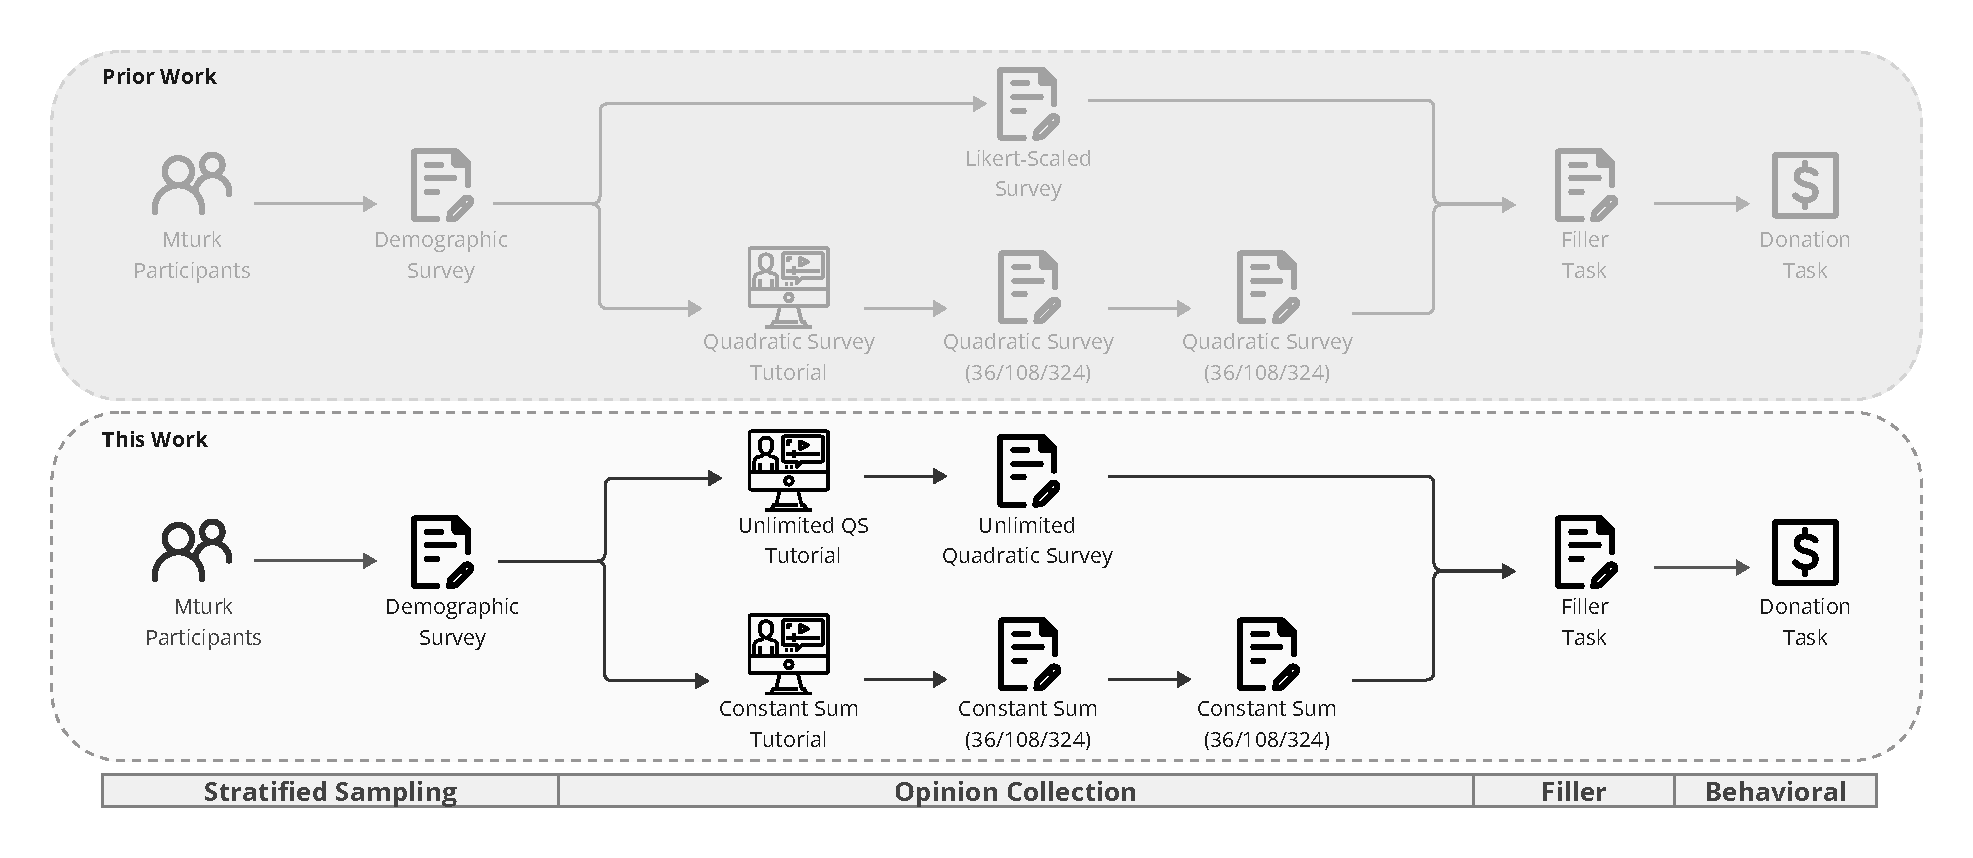
\includegraphics[width=\textwidth]{content/image/whyqs_exp_flow.pdf}
    \caption{Experiment overview. Our study covers the dotted box beneath, mirroring prior research only differing the type of surveys involved during the opinion collection section. The bar below highlights the four parts of the study: sampling, opinion collection, filler task, and the behavioral task.}
    \label{fig:experiment}
\end{figure}

\subsection{Experiment Design}
To ensure comparability with the prior study~\cite{chengCanShowWhat2021}, we followed the same between-subject experimental design and modified open-source software to introduce two new condition types, yielding four additional experimental datasets. The subsections below highlight key procedural modifications, while the choice of survey methods and the donation task are justified by prior research. Figure~\ref{fig:experiment} illustrates how our study fits within the broader experimental flow established by previous work.

\paragraph{Additional Experimental Conditions}
We introduced four new experimental conditions, grouped into two categories: UQS and LS. In the UQS condition, we removed the budget constraint to isolate the effect of the quadratic cost function. In the LS conditions, we replaced the quadratic cost function with a linear one and further subdivided these into three levels based on budget size:

\begin{itemize} 
    \item LS18: A small-budget Linear Survey with 18 credits
    \item LS54: A medium-budget Linear Survey with 54 credits
    \item LS162: A large-budget Linear Survey with 162 credits
\end{itemize}

Following prior work, we allocated two credits per option to match the expressiveness of a 5-point Likert scale, allowing participants to indicate moderate intensity in either direction. With nine options, this yielded 18 credits for the LS18 condition. We then scaled the budgets using $O(K)$, $O(K^{1.5})$, and $O(K^2)$ to generate LS18, LS54, and LS162, respectively—for example, $2 \times 9^{1.5} = 54$ in LS54.

\subsubsection{Survey content}
The study frames the survey as a public resource allotment task, where participants express preferences across 9 societal issues such as education, environment, or health. Participants would express their degree of preference in the number of votes, positive or negative, under the mechanism of UQS or LS.

\subsubsection{Surveying process and interface}
Participants in both groups were first introduced to the survey and how to use it via a video tutorial. To ensure their understanding of the survey mechanism, participants were asked to complete a quiz with 5 multiple-choice questions. Participants had to answer at least three questions correctly to continue the study. We altered the questions based on the survey mechanisms. The interface for both UQS and LS are shown in~\Cref{fig:extended_interface}.

% create a side by side figure using subfigure

\begin{figure}
    \centering
    \begin{subfigure}{0.47\textwidth}
        \centering
        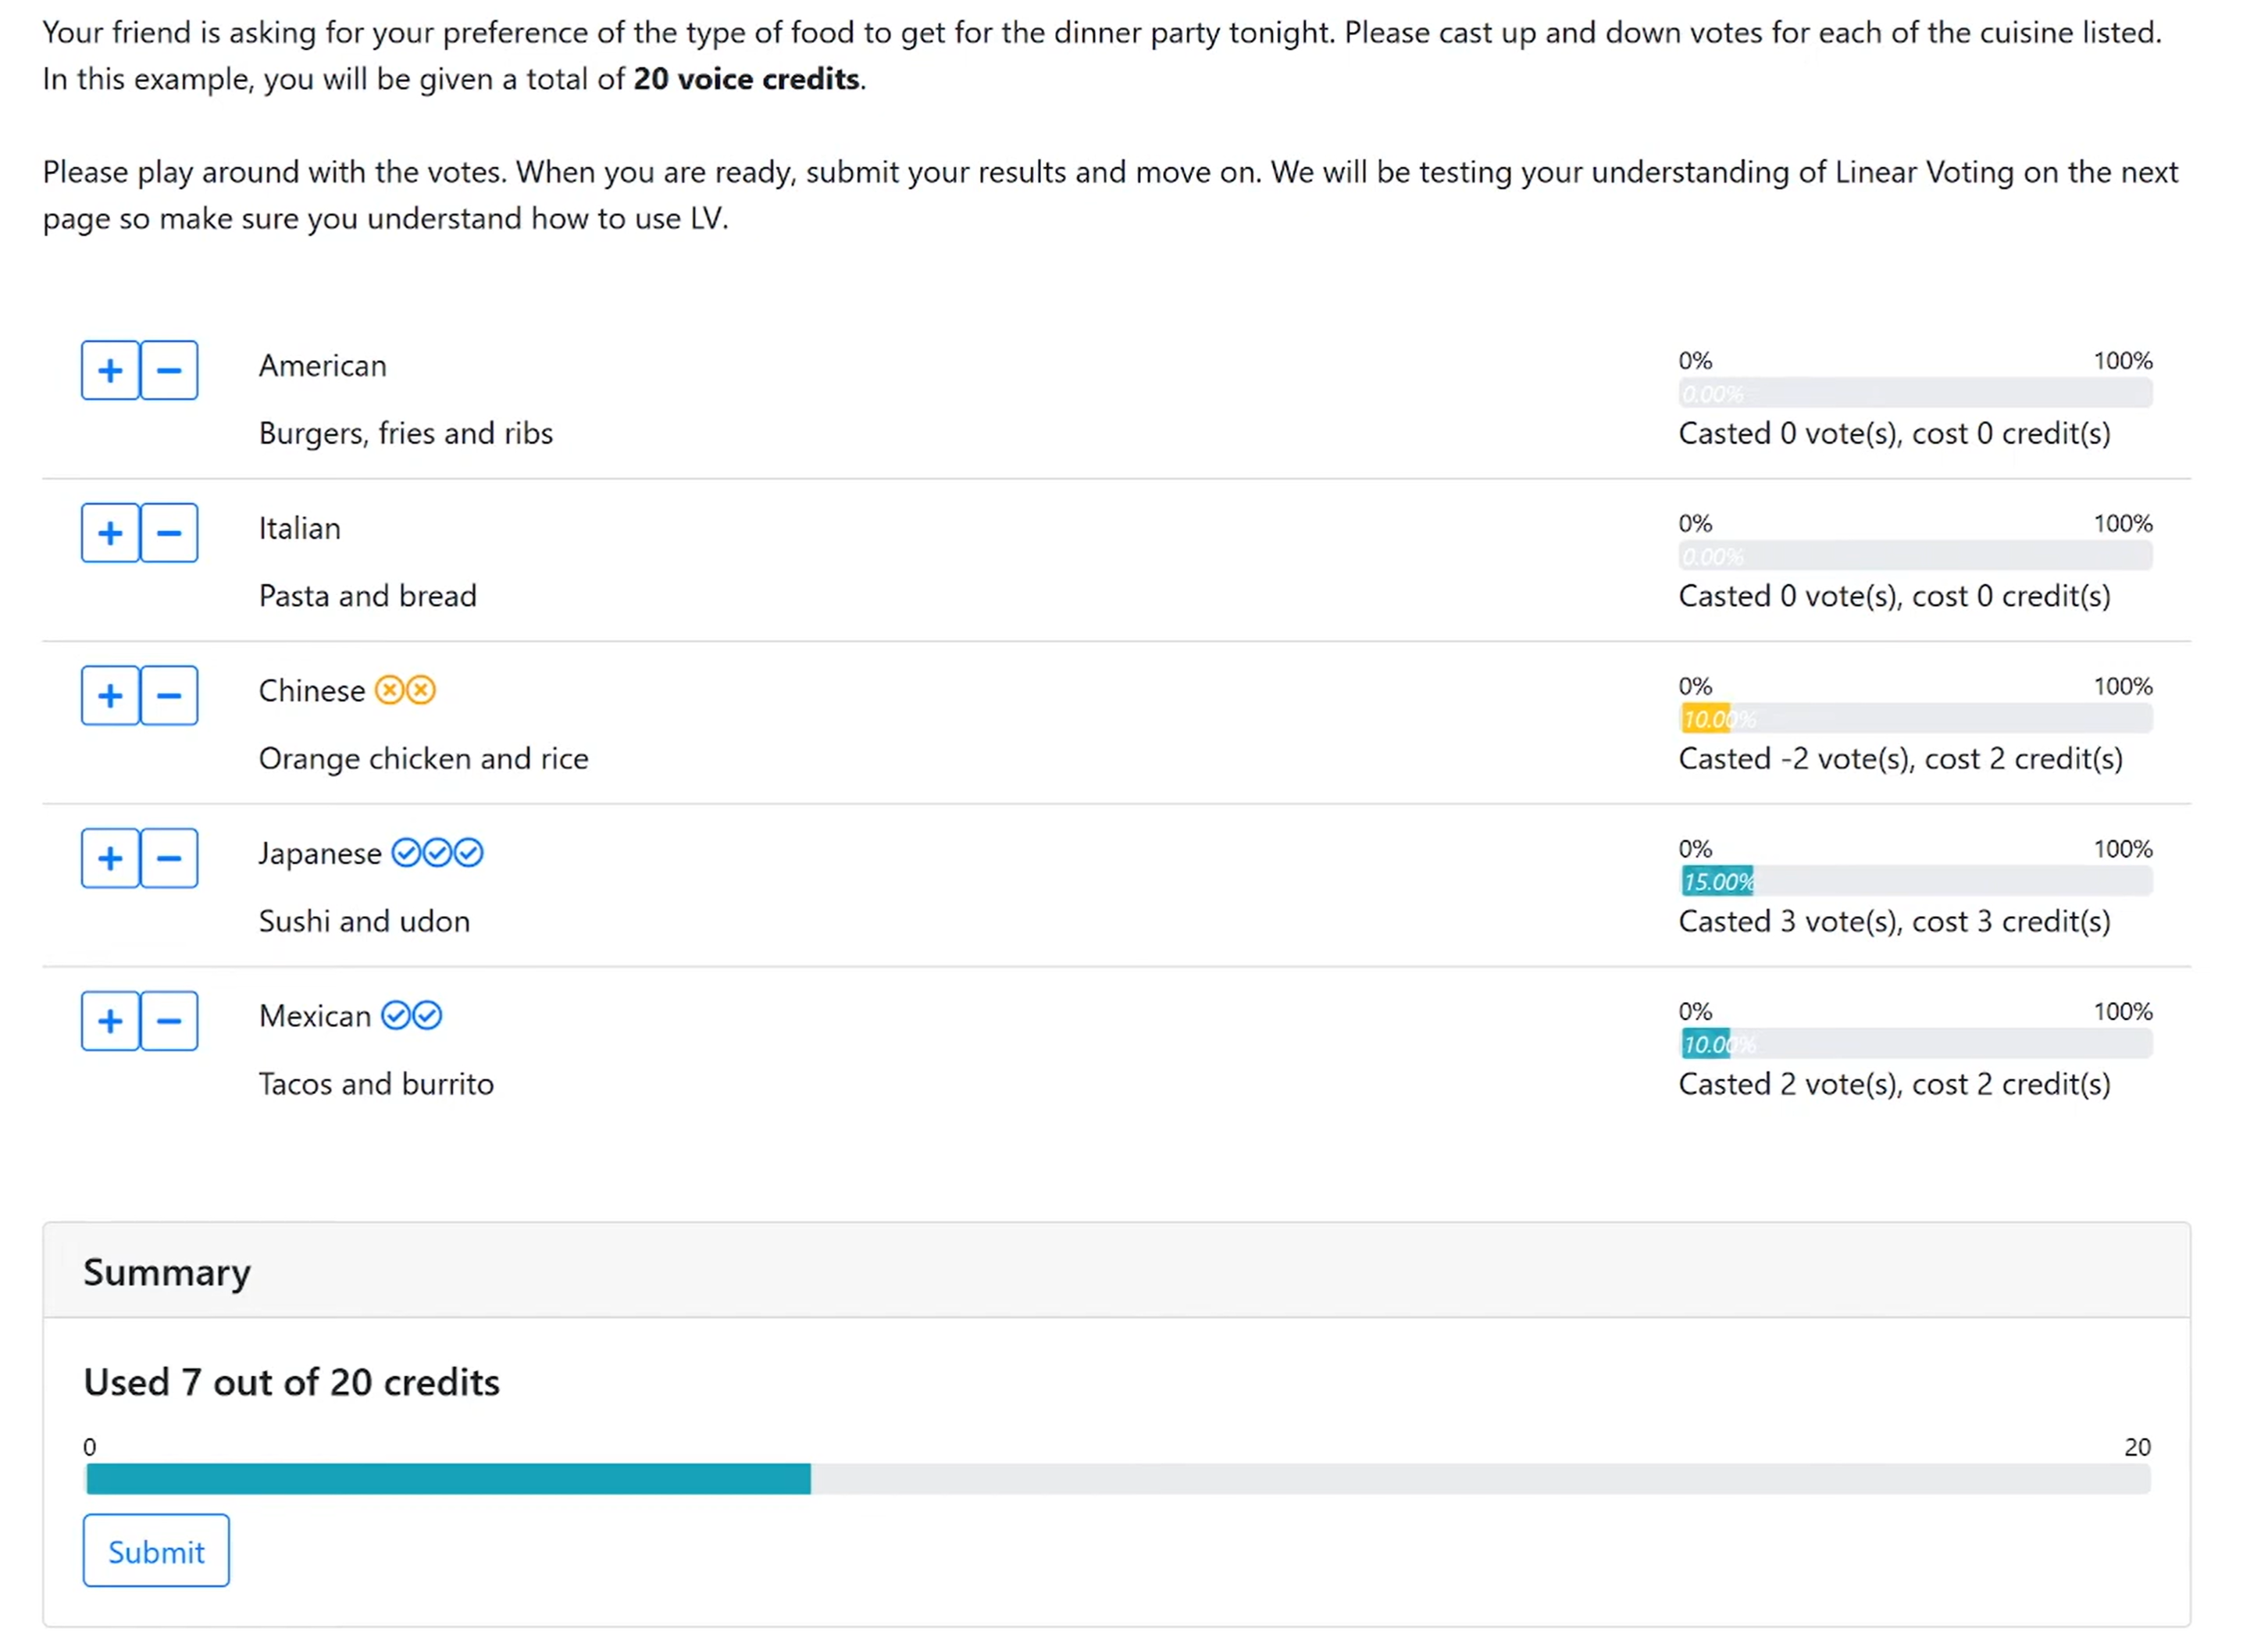
\includegraphics[width=\textwidth]{content/image/linear.png}
        \caption{Linear Survey (QS) Interface, each additional vote is $1$ credit}
        \label{fig:qs_interface}
    \end{subfigure}
    \hfill
    \begin{subfigure}{0.47\textwidth}
        \centering
        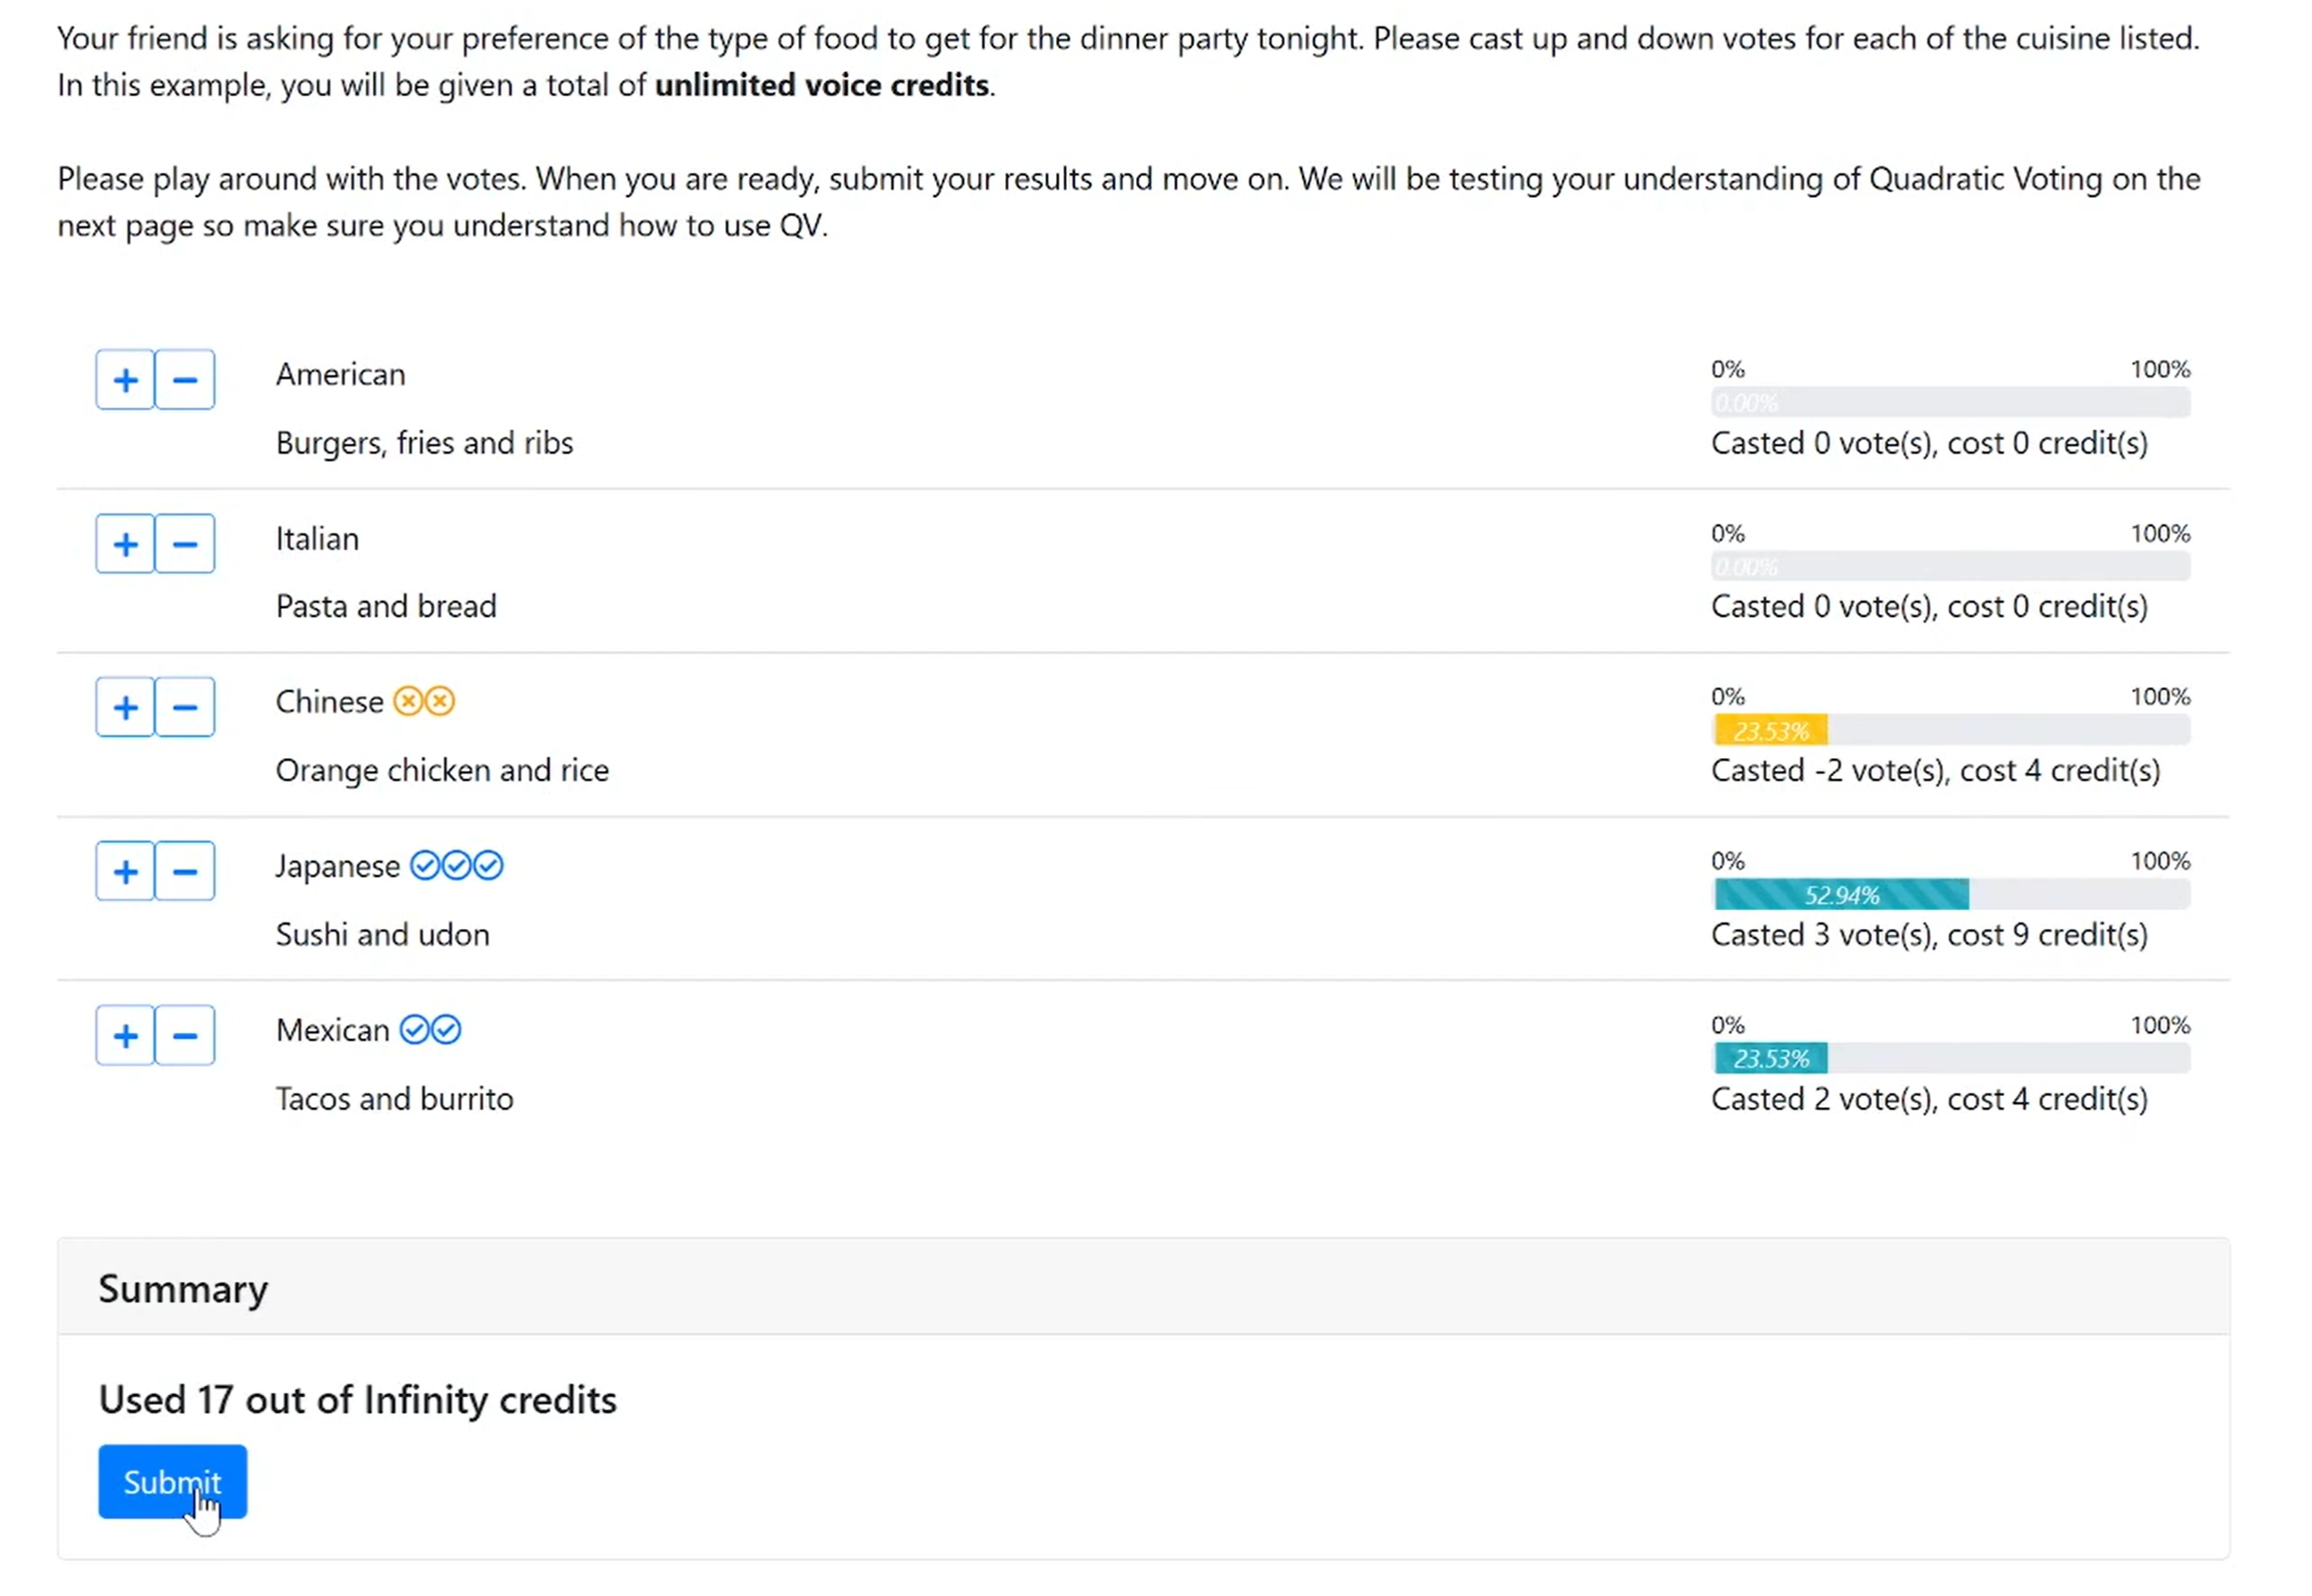
\includegraphics[width=\textwidth]{content/image/uqs.png}
        \caption{Unlimited Quadratic Survey (UQS) Interface, each additional vote is $n^2$ credits but does not have a budget constraint}
        \label{fig:css_interface}
    \end{subfigure}
    \caption{Survey interfaces for the two additional conditions. Both images are screenshots of the playground for participants to experience the surveying method before completing the actual survey tasks on societal issues.}
    \label{fig:extended_interface}
\end{figure}


\subsubsection{Filler task and donation}
After the survey, participants completed a filler task to prevent direct association with the issues and the charities listed on the donation task page. Participants 

\subsubsection{Debrief, and Compensation}
After the study, participants have a chance to read about the study's real purpose on the debrief page. Participants were compensated with \$1.50 for their time, and they were informed that they would receive an additional \$0.50 if they completed the study.

\subsubsection{Integrating prior data}
\citet{chengCanShowWhat2021} was the first study to evaluate the effectiveness of QS in relation to human behavior, offering an open dataset and open-source software that we replicated and extended. Their dataset contains 219 MTurk participants: 56 completed a Likert scale survey, 107 completed the QS36 survey, 108 completed QS108, and 111 completed QS324.

To facilitate our analysis, we differentiate between the number of votes allocated to each option (used in the original QS analysis) and the total credits spent on each option, which reflects the actual cost incurred under the quadratic cost function. To make this distinction clear, we refer to the credit-spent measures as QSC36, QSC108, and QSC324, corresponding to the cost-based modeling of QS36, QS108, and QS324 conditions.

Altogether, this study compares the elicited preferences from QS (vote-based), QSC (cost-based), LS (linear cost), UQS (QS without budget constraints), and Likert scale surveys, using participants' actual donation behavior as a behavioral baseline. These conditions are summarized in~\Cref{tbl:experiment_cond}.


\begin{table}[h]
    \centering
    \begin{tabular}{@{}lllp{9cm}@{}}
        \toprule
        \textbf{Condition} & \textbf{Budget} & \textbf{Cost Function} & \textbf{Description} \\
        \midrule
        Likert & – & – & A 5-point traditional ordinal-scale survey. \\ 
        \midrule
        Donation & – & – & Incentive-compatible donation task used as behavioral benchmark for validating expressed preferences. \\
        \midrule
        QS36   & 36   & Quadratic & \multirow{3}{9cm}{QS conditions with three different budgets ($O(K)$, $O(K^{1.5})$, $O(K^2)$). Participants expressed preferences by allocating votes, where the cost of each vote increased quadratically, deducted from the budget.} \\
        QS108  & 108  & Quadratic & \\
        QS324  & 324  & Quadratic & \\
        \midrule
        QSC36  & 36   & Quadratic & \multirow{3}{9cm}{Credits that participants contributed per option. Using the results from QS, QSC reflects the actual cost incurred per option to reflect perceived intensity of preference and explore alignment with donation outcomes.} \\
        QSC108 & 108  & Quadratic & \\
        QSC324 & 324  & Quadratic & \\
        \midrule
        LS18   & 18   & Linear    & \multirow{3}{9cm}{Linear-cost versions of QS with budgets scaled as $O(K)$, $O(K^{1.5})$, and $O(K^2)$. Participants expressed preferences by allocating votes, where the cost of each vote increased linearly, deducted from the budget.} \\
        LS54   & 54   & Linear    & \\
        LS162  & 162  & Linear    & \\
        \midrule
        UQS    & Unlimited & Quadratic & QS without a budget where participants expressed preferences by allocating votes, where the cost of each vote increased quadratically but there is not budget that they ahere to. \\
        \bottomrule
    \end{tabular}
    \caption{Summary of experimental and behavioral conditions, their cost structures, budget levels, and modeling purposes.}
    \label{tbl:experiment_cond}
\end{table}

\subsection{Quantitative Measures: Ordinal and Interval Measures}
\label{sec:quantitative_measures}
Two prior empirical studies compared elicited survey responses with behavioral outcomes—such as donation~\cite{chengCanShowWhat2021,cavaille2024cares} or letter length~\cite{cavaille2024cares}—as proxies for individual preferences. ~\citet{chengCanShowWhat2021} employed a Bayesian model to compute cosine similarity, which measures the alignment between participants' stated preferences and observed behaviors. ~\citet{cavaille2024cares} used linear regression to estimate the differences between stated preferences and behavioral outcomes.

While cosine similarity is useful for high-dimensional data, it poses interpretative challenges. For example, high alignment might result from large angular differences between vectors with identical rankings, whereas low alignment could stem from small angular differences between completely misaligned rankings. Linear regression, by contrast, primarily captures correlations rather than causal relationships, limiting its explanatory power. Additionally, since each behavioral measure (e.g., donation, letter writing) represents a distinct task, comparing relative preferences across options within the same participant is difficult.

Thus, in this study, we draw from prior literature to compare multi-option survey instruments by breaking down and evaluating QS's ability to elicit ordinal and interval scales separately~\cite{collewetPreferenceEstimationPoint2023}. We construct Bayesian models for both analyses, considering their transparency in interpreting posterior distributions beyond binary thresholds~\cite{mcelreath2018statistical, kay2016researcher}. We compare five different conditions and describe the models in the following subsections.

\subsubsection{Pairwise Ordinal Measures}
\label{sec:ordinal_measures}
The first analysis, which we termed~\textbf{sign analysis}, focuses on understanding how the outcomes from different instruments align with participants' donation behavior in terms of preference order. To achieve this, we construct pairwise comparisons between the two sets. 

After removing participants that made zero donations, for each pairwise option on a survey, we modeled $y_i$ as the outcome variable of whether the order of the two options expressed through the instrument aligns with the order of the donated amount. In other words, our model learns how well does a given survey instrument capture the preference between two options with their donation amount? Since the possible outcome would be either align or misaligned ($\pm 1$), we modeled the outcome variable $y_i$ as a Bernoulli distribution (Equation~\ref{eq:ordinal_model_overall}).

\begin{equation}
    \label{eq:ordinal_model_overall}
    y_i \sim \text{Bernoulli}(\theta_i)
\end{equation}

\begin{equation}
    \label{eq:ordinal_model_logit}
    \text{logit}(\theta_i) = \alpha + \beta_c[C_i] + \beta_o[O_i] + \beta_p[P_i] + \beta_t[T_{1i}] + \beta_t[T_{2i}]
\end{equation}

The model $\theta_i$ is modeled as a logit function (Equation~\ref{eq:ordinal_model_logit}) between pairwise topics $T_{1i}$ and $T_{2i}$, which we control for the specific survey instrument $C_i$. We also control for the order for which participants complete the survey in the QS and LS conditions, denoted as $O_i$ and if so, if the participants was already aligned in a prior condition, $P_i$. The latter two experiment variable help control for potential learning effects since the two survey only differ in the number of provided budgets.

We applied a hiarchical approach to model these experimental variables with a non-centered parameterization~\cite{mcelreath2018statistical}. The hierarchical approach allows partial polling across different pairwise comparisons (e.g., considering how the participants consider the same pair of topics), while preventing overfitting. With so many experimental variables to model under this setup, we applied a non-centered parameterization allows the model to learn the distribution of the parameters from the data rather than being overly constrained by the priors~\cite{mcelreath2018statistical}. This yields more robust inferences, improves sampling efficiency and stability of the model.

This means that for each experimental variable, it follows Equation~\ref{eq:generic_non_center_hyper} where the different possible values of the variable are modeled as a normal distribution with mean $\mu_x$ and standard deviation $\sigma_x$.

\begin{equation}
    \label{eq:generic_non_center_hyper}
    x_i = \mu_x + \sigma_x \cdot \eta_i, \quad \eta_i \sim \mathcal{U}(0,1)
\end{equation}

Each sigma is drawn from a normal distribution with different hyperpriors for each variable. For example, $C_i$ which represents different experiment condition's survey instrument follow the following model:

\begin{align}
    \label{eq:generic_non_center_hyper_C}
    \beta_c[c_i] = \beta_a + \sigma_c \cdot \eta[c_i]\\
    \quad \sigma_c \sim \mathcal{U}(0,1)\\
    \quad \beta_a \sim \mathcal{N}(0, 0.5)\\
    \quad \eta[c_i] \sim \mathcal{N}(0, 1)
\end{align}

The rest of the experimental variables follows the same structure, with the only difference in the hyperprior distribution $\mu_x$. For example, the topics $T_{1i}$ and $T_{2i}$ has a hyperprior of $\mathcal{N}(0, 0.25)$, while the rest of the experimental variables have a hyperprior of $\mathcal{N}(0, 0.5)$. 

\subsubsection{Interval Measures}
\label{sec:interval_measures}
Following the ordinal comparisons,~\textbf{intensity model} assesses how effectively instruments capture the magnitude of preference differences between options. This model evaluates how well an instrument reflects varying degrees of preference along a continuum.

\paragraph{Aligning the variables} Constructing a intensity model to compare the different instruments is not trivial, since elicited values are continuous and others are ordinal. We took a conservative approach and model Likert scale and QS votes as ordinal values, especially when it is not clear whether participants considering the varying costs associated with different votes for the latter. In contrast, LS reflects incremental additions on a scale, and UQS does not have a limit; hence, both are treated as continuous. Rather than solely using final outcomes from each instrument, we also incorporated the cost of votes for QSs, assuming each dollar increment shares the same ``monetary'' value.

For instruments with bounded, continuous budgets (e.g., \textit{QSC\_36}, \textit{QSC\_108}, \textit{QSC\_324}) and linear surveys (\textit{LS\_18}, \textit{LS\_54}, \textit{LS\_162}), we project vote differences onto the $[0,1]$ interval. Since UQS lacks fixed bounds, we normalize the vote difference $V$ between two options $t_1$ and $t_2$ over the $k'$ options that the participant voted on:

\begin{equation}
    \text{Vote\_diff}_{UQS} 
    = (V_{t1} - V_{t2})/\textstyle\sum V_{k'}
\end{equation}
and apply the same normalization for UQS credits.

\paragraph{Projecting Ordinal values} 
To facilitate a direct comparison, we transform the ordinal results into an unobserved latent continuous variable using a Dirichlet-based ``cutpoint'' transformation. Specifically, for each instrument, we derive $K$ discrete ordinal \emph{difference} categories. For example, QS36 has 17 possible difference categories (ranging from $-8$ to $+8$)\footnote{Here, 36 credits can generate a largest difference of 5 votes vs.\ $-3$ votes.}. We then sample
\(\boldsymbol{\alpha}\) from a Dirichlet$(\mathbf{1}\cdot\delta)$ prior, where each of its $K-1$ positive components sums to 1:

\begin{equation}
    \boldsymbol{\alpha} \sim \mathrm{Dirichlet}\bigl(\mathbf{1}\cdot \delta\bigr)
\end{equation}

We modeled the distribution with $\delta=2$ as a weakly informative prior over the latent cutpoints. We pad this vector so that $\alpha_0 = 0$, then map each category $k$ to a latent continuous value:

\begin{equation}
    x_{\mathrm{latent}}^{(k)} = \sum_{j=0}^{k} \alpha_j.
\end{equation}

As $k$ increases, $x_{\mathrm{latent}}^{(k)}$ grows but remains within the $[0,1]$ interval, effectively assigning each ordinal category a continuous value. 

\paragraph{Projecting Donations} Finally, since donation amounts also vary by participant, we remove those who donated nothing and normalize each donation difference by the participant's total donation, mirroring our UQS approach. With these transformations, all experimental variables and outcomes lie in $[0,1]$, forming the basis for a \emph{hierarchical normal} model.

\paragraph{Modeling the outcome}
We seek to capture how an instrument \emph{predicts} the donation difference $y_i$ between two options. Conditional on a mean $\mu_i$, the outcome follows a normal distribution:

\begin{equation}
    \label{eq:intensity_normal}
    y_i \sim \mathcal{N}(\mu_i, \sigma_i).
\end{equation}

where $C_i$ denotes the survey instrument (Likert, QS, QS cost, LS, or UQS). We place a prior $\mathcal{N}(0,0.2)$ on the intercept $\beta_{c}[C_i]$ for each condition and use a non-centered parameterization~\cite{mcelreath2018statistical} to model condition-specific slopes:

\begin{equation}
    \beta_{\text{vote}}[C_i]
    \;=\;
    \beta_{\text{vote}\,\text{bar}}
    + \sigma_{\text{vote}}\,\eta_{\text{vote}}[C_i],
    \quad
    \beta_{\text{vote}\,\text{bar}}
    \sim
    \mathcal{N}(0,1),
    \quad
    \sigma_{\text{vote}}
    \sim
    \mathrm{Uniform}(0,1),
    \quad
    \eta_{\text{vote}}[C_i]
    \sim
    \mathcal{N}(0,1).
\end{equation}

These slopes, together with each instrument's intercept, determine how normalized vote differences $\text{VoteDiff}_i$ (either transformed ordinal or inherently continuous) map onto $y_i$. We also include an order effect $\beta_{o}[O_i]$ and topic intercepts $\beta_{t}[T_{1i}]$ and $\beta_{t}[T_{2i}]$, each following a non-centered prior with a Normal hyper-mean and a Uniform hyper-scale. Putting these elements together, the linear predictor is:

\begin{equation}
    \label{eq:intensity_linpred}
    \mu_i
    =
    \beta_{c}[C_i]
    +
    \beta_{\text{vote}}[C_i] \cdot \text{VoteDiff}_i
    +
    \beta_{o}[O_i]
    +
    \beta_{t}[T_{1i}]
    +
    \beta_{t}[T_{2i}].
\end{equation}

Each condition is then assigned its own standard deviation $\sigma_i=\beta_{\sigma}[C_i]$, where $\beta_{\sigma}[C_i]$ is drawn from an $\mathrm{Exponential}(1)$ prior. Hence, different instruments exhibit distinct variance in donation differences.

A hierarchical Bayesian approach ties all these parameters together via a non-centered parameterization:

\begin{equation}
    x_i
    =
    \mu_x
    + \sigma_x \cdot \eta_i,
    \qquad
    \eta_i
    \sim
    \mathcal{N}(0,1).
\end{equation}

Here, $\mu_x$ and $\sigma_x$ define the group-level mean and scale for each parameter type, and $x_i$ represents condition intercepts, slopes, order intercepts, or topic intercepts. By integrating condition, vote difference, order, and topic effects into a single hierarchical normal framework, our model provides a structured way to analyze how different survey instruments capture the intensity of preference differences.


\section{Modeling for Pairwise Ranking and Preference Intensity Analyses}
\label{sec:quantitative_measures}
Two recent empirical studies have evaluated whether elicited survey responses align with participant behavior, using outcomes such as charitable donations~\cite{chengCanShowWhat2021, cavaille2024cares} or letter-writing effort~\cite{cavaille2024cares} as behavioral proxies for underlying preferences. One approach used Bayesian cosine similarity to compare high-dimensional response vectors with behavioral outcomes~\cite{chengCanShowWhat2021}; another applied linear regression to estimate the gap between stated and revealed preferences~\cite{cavaille2024cares}.

However, cosine similarity poses interpretability challenges: vectors with identical pairwise rankings can still be judged dissimilar, while near-aligned vectors may reflect contradictory preferences. Moreover, distinct behavioral measures (e.g., donations vs. letter writing) complicate comparisons of pairwise preferences across options within the same participant.

To address these limitations, we evaluate survey instruments based on their ability to recover (1) \textit{pairwise preference rankings} and (2) \textit{preference intensity differences} between options, within participants. This dual evaluation draws from methods used in studies of point-allocation and forced-choice surveys~\cite{collewetPreferenceEstimationPoint2023}, and allows us to separately assess ordinal and interval-level performance. 

We employ Bayesian modeling in both cases to support transparent assumptions, account for uncertainty, and enable interpretation beyond binary significance thresholds~\cite{mcelreath2018statistical, kay2016researcher}. The two models are described below.

\subsection{Pairwise Ranking Model}
\label{sec:ordinal_measures}
Our first analysis evaluates how well different survey instruments capture pairwise rankings that align with those inferred from actual donation amounts. We model the binary observation ($y_i$) of whether a participant $i$'s pairwise ranking expressed via the survey instrument matches that from the donation results for a given societal issue pair as a Bernoulli distribution in \Cref{eq:ordinal_model_overall}:

\begin{equation}
    \label{eq:ordinal_model_overall}
    y_i \sim \text{Bernoulli}(\theta_i)
\end{equation}

The alignment probability, $\theta_i$, is defined using a logit link function (Equation~\ref{eq:ordinal_model_logit}) and modeled as a function of several experimental variables:

\begin{equation}
    \label{eq:ordinal_model_logit}
    \text{logit}(\theta_i) = \alpha + \beta_c[C_i] + \beta_o[O_i] + \beta_p[P_i] + \beta_t[T_{1i}] + \beta_t[T_{2i}]
\end{equation}

The variables represent experimental conditions and relevant controls. Specifically, $C_i$ denotes the survey instrument, spanning eight conditions (see \Cref{tbl:experiment_cond}\footnote{Since this model only considers pairwise rankings, UQS and QS votes and credits yield the same result.}): three QS variants with different budgets, three LS variants with different budgets, Likert scale survey, and UQS. Since some participants worked on multiple survey instruments, $O_i$ captures the order in which the participant completed survey $C_i$ to account for ordering effects. In addition, $P_i$ represents whether a participant’s pairwise ranking in an earlier survey aligned with the donation-based ranking, accounting for carryover effects. Lastly, $T_{1i}$ and $T_{2i}$ account for the topic-level effects of the two issues in comparison.

Given the complexity and nested structure of the data, we used a hierarchical Bayesian logistic regression model with non-centered parameterization~\cite{mcelreath2018statistical}. Hierarchical modeling enables partial pooling across different experimental conditions or topic pairings, which improves estimate robustness~\cite{mcelreath2018statistical}. 

The coefficients of each experiment variable ($\beta_{c}$, $\beta_{o}$, $\beta_{p}$, and $\beta_{t}$) are modeled using a hierarchical structure, drawn from a normal distribution centered at a group-level mean $\mu_{\beta}$ and scaled by a group-level standard deviation $\sigma_{\beta}$. For example, the hierarchical structure of coefficient $\beta_c$ for the survey condition variable $C_i$ is defined as: 

\begin{align}
    \label{eq:generic_non_center_hyper_C}
    \beta_c[C_i] &= \mu_{\beta_c} + \sigma_{\beta_c} \cdot \eta[C_i], \quad \eta[c_i] \sim \mathcal{N}(0, 1) \\
    \mu_{\beta_c} &\sim \mathcal{N}(0, 0.5), \quad   \sigma_c \sim \mathrm{Uniform}(0,1) 
\end{align}

Other coefficients follow the same structure, but some have different hyper-priors. Specifically, topic coefficients $\beta_{t}$ use a narrower hyper-prior $\mu_{\beta_t} \sim \mathcal{N}(0,0.25)$ to reflect a smaller expected effect.



\subsection{Pairwise Preference Intensity Model}
\label{sec:interval_measures}
The pairwise intensity model evaluates how effectively each survey instrument captures the magnitude of preference differences between options. We seek to model how the response difference between two options on a survey $\Delta_{\text{Survey}}$ \emph{predicts} the donation difference $\Delta_{\text{Donation}}$. Besides the eight survey conditions in the pairwise ranking model, we additionally analyze the number of credits spent on an option in QS (three budgets) and UQS (\Cref{tbl:experiment_cond}).

Comparing preference differences elicited via various survey instruments ($\Delta_{\text{Survey}}$) to donations ($\Delta_{\text{Donation}}$) is not trivial since some yielded continuous data while others were ordinal. Following the convention, we model $\Delta_{\text{Likert}}$ as ordinal data. Given the uncertainty about how participants accounted for the varying costs associated with QS votes, we treat $\Delta_{\text{QS Vote}}$ as ordinal as well. In contrast, LS votes increment with a consistent cost on a scale and are therefore modeled as a continuous variable. UQS has no upper limit; hence, it is not ordinal. Finally, QS credits and monetary donations are continuous by nature.

Another challenge of this comparison is that raw differences from various instruments ($\Delta_{\text{Survey Raw}}$) and $\Delta_{\text{Donation Raw}}$ fall into varying data ranges. Thus, we apply the following data normalizations.

\paragraph{Normalize Continuous Survey Difference} We apply a variation of min-max scaling to project continuous $\Delta_{\text{Survey Raw}}$ onto the $[-1,1]$ interval\footnote{$\frac{x-min(x)}{(max(x) - min(x))}\times 2 - 1$}. For QS credits and LS, we use the predefined bounds as the $min$ and $max$ in scaling. Since UQS lacks fixed bounds, we calculate the $min$ and $max$ for each participant based on the total votes and credits they used.

\paragraph{Normalize Ordinal Survey Difference} 
To enable direct comparison with continuous data, we project ordinal difference categories onto a latent continuous scale between 0 and 1, using cutpoints drawn from a Dirichlet-based model. Specifically, for each instrument, we derive $K$ discrete ordinal \emph{difference} categories. For example, vote difference in QS36 has 17 possible difference categories ($\Delta_{\text{QS36 Vote Raw}} = [-8, -7, ..., 7, 8]$)\footnote{Here, the largest vote difference possible with 36 credits occurs with 5 votes on option A and $-3$ votes on option B.}. We sample the second to $K$th elements of cutpoints \(\boldsymbol{\alpha}\) from a Dirichlet$(\mathbf{1}\cdot\delta)$ with $\delta=2$ as a weakly informative prior so that they sum to 1:

\begin{equation}
    \boldsymbol{\alpha}_{[2, ...,K]} \sim \mathrm{Dirichlet}\bigl(\mathbf{1}\cdot \delta\bigr), \text{where } \delta = 2
\end{equation}

The first cutpoint is $\alpha_{1} = 0$. We then map ordinal $\Delta_{\text{Survey Raw}}=k$ to a latent continuous value between $[0,1]$ as $\Delta_{\text{Survey}}$:

\begin{equation}
    \text{For }\Delta_{\text{Survey Raw}}=k\text{, } \Delta_{\text{Survey}} = \sum_{j=1}^{k} \alpha_j.
\end{equation}

\paragraph{Normalize Donation Difference} Finally, we apply the same variation of min-max scaling to the donation differences of each participant based on their total donation amount. $\Delta_{\text{Donation}}$ ranges from $[-1, 1]$.

\textbf{Model Specification:} We model $\Delta_{\text{Donation}}$ as a Normal distribution:

\begin{equation}
    \label{eq:intensity_normal}
    \Delta_{\text{Donation}_i} \sim \mathcal{N}(\mu_{D_i}, \sigma_{D_i}).
\end{equation}

Since it is reasonable to expect that the variance in donation differs across experimental conditions, we make 
$\sigma_{D_i}$ condition-dependent: $\sigma_i=\beta_{\sigma}[C_i]$, where $\beta_{\sigma}[C_i]$ is drawn from the prior $\mathrm{Exponential}(1)$. $\mu_{D_i}$ is predicted by a linear regression of survey response difference $\Delta_{\text{Survey}_i}$, survey instrument $C_i$, survey order $O_i$, and topics $T_{1i}$, $T_{2i}$. 

\begin{equation}
    \label{eq:intensity_linpred}
    \mu_i
    =
    \beta_{\text{S}}[C_i] \cdot \Delta_{\text{Survey}_i}
    +
    \beta_{c}[C_i]
    +
    \beta_{o}[O_i]
    +
    \beta_{t}[T_{1i}]
    +
    \beta_{t}[T_{2i}].
\end{equation}

We model the slope of survey response differences $\beta_{\text{S}}$ for each survey condition with partial pooling and non-centered parameterization.

\begin{align}
    \beta_{\text{S}}[C_i]
    &=
    \mu_{\beta_{\text{vote}}}
    + \sigma_{\beta_{\text{vote}}} \cdot \eta_{\beta_{\text{vote}}}[C_i],
    \quad \eta[c_i] \sim \mathcal{N}(0, 1) \\
    \mu_{\beta_{\text{vote}}}
    &\sim
    \mathcal{N}(0,1),
    \quad
    \sigma_{\beta_{\text{vote}}}
    \sim
    \mathrm{Uniform}(0,1).
\end{align}

We model intercepts $\beta_{o}$ and $\beta_{t}$ in a similar way but with a hyper-prior of $\mu_{\beta} \sim \mathcal{N}(0,0.1)$. Finally, we sample the condition-based intercept $\beta_{c}$ from the prior $\mathcal{N}(0,0.2)$ without pooling. 

\section{Results}
We present findings on pairwise rankings and preference intensity in Section~\ref{sec:result_1} and Section~\ref{sec:result_2}, respectively.

\begin{figure*}[h]
    \centering
    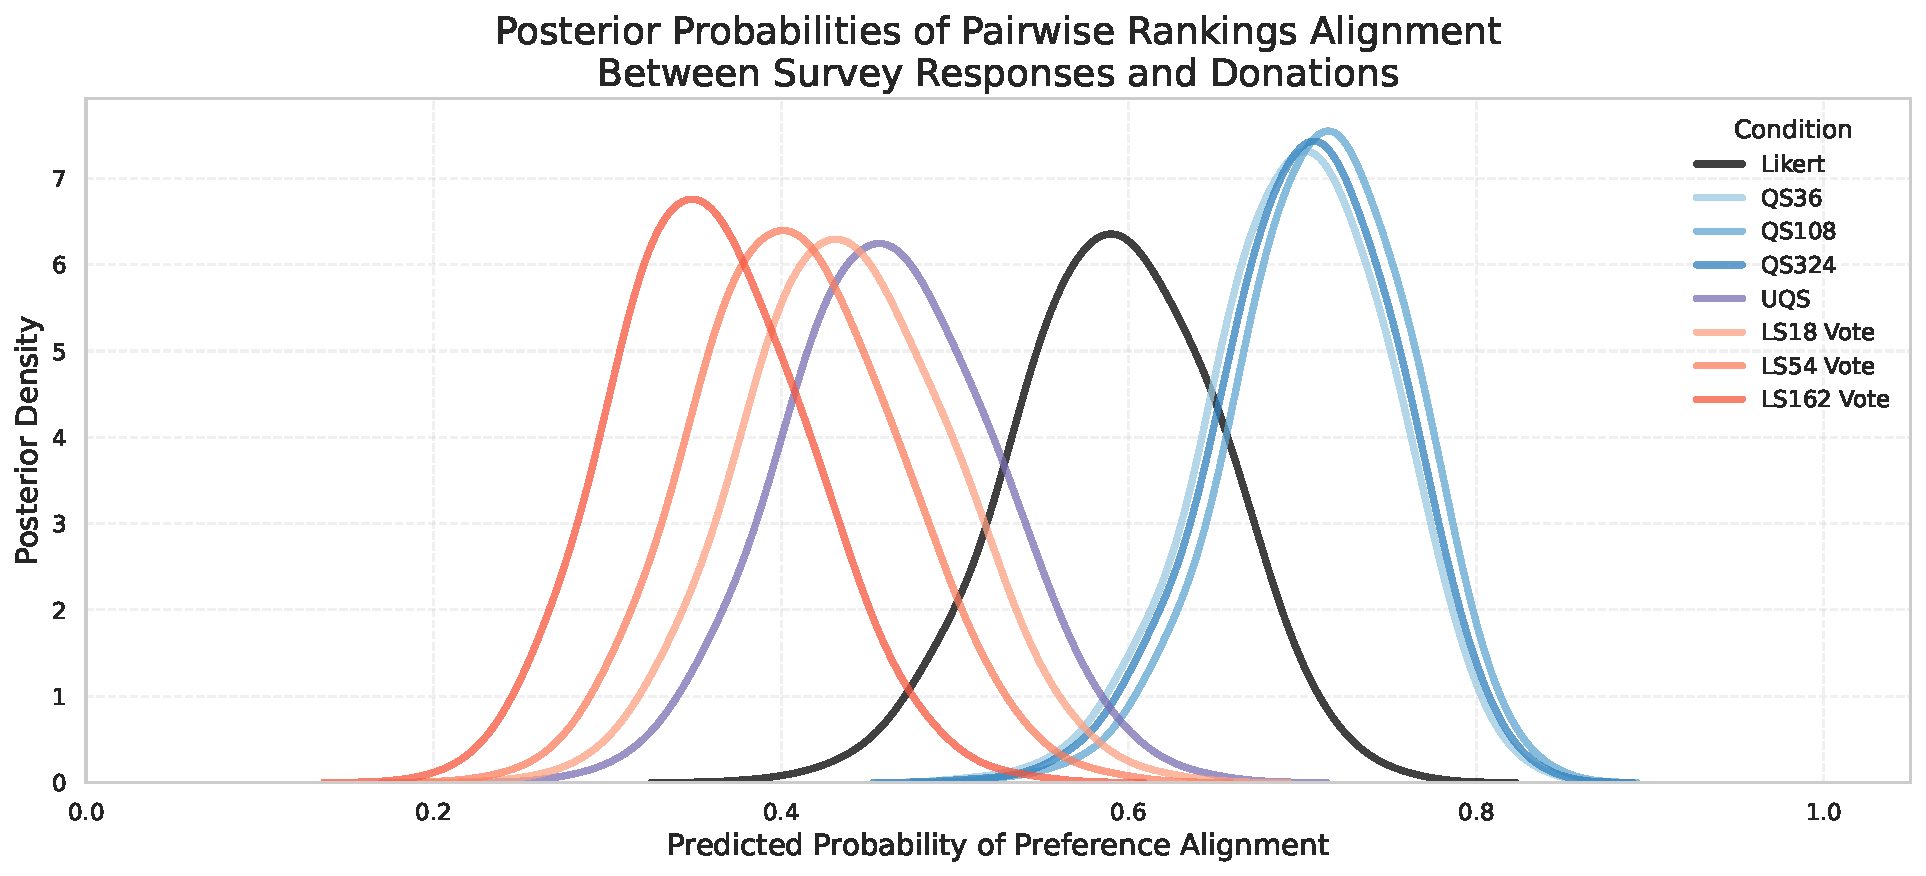
\includegraphics[width=\textwidth]{content/image/overlapping_density_custom_palette.pdf}
    \caption{
    This figure presents the posterior density distributions of the probability that pairwise rankings from various survey tools align with participants' actual donation behavior. The x-axis shows the predicted probability of correct pairwise ranking alignment, where 1 indicates perfect alignment. The y-axis represents the posterior density across the sampled distribution. Each curve corresponds to a different survey condition. QS with varying budgets cluster together, exhibiting higher alignment probabilities as reflected by their distributions peaking further to the right. In contrast, UQS and LS show lower alignment, with LS performance declining as its budget increases. \textbf{Main takeaway:} Budget-constrained QS elicit pairwise rankings that align more closely with participants' donation behaviors, highlighting their effectiveness in capturing directional preferences.}
    \label{fig:ranking_posterior}
\end{figure*}

\subsection{Pairwise Preference Ranking Results}
\label{sec:result_1}

\textbf{Results interpretation: }To evaluate how well a survey tool reflects a participant's preference ranking between two causes, we calculate the posterior distribution of the probability that the pairwise preference ranking reflected through a survey tool aligns with that reflected in donation amounts (\Cref{fig:ranking_posterior}). Furthermore, we compare survey tools' abilities to elicit accurate pairwise preference rankings using the odds ratio of the predicted odds of alignment between survey and donation preference rankings. For instance, an odds ratio of 2 between survey tools A and B means that the odds of participants expressing the same preference rankings in survey tool A and donations is twice those of participants using survey tool B. We say that two survey tools differed significantly when the 94\% Highest Posterior Density Interval (HPDI) of the odds ratio's posterior distribution does not include the reference value of 1 (odds ratio = 1 means having the same odds). 

\textbf{QS outperformed the Likert scale survey in eliciting preference rankings consistent with donations, with a small effect size} (odds ratio mean = 1.65, 94\% HPDI = [1.55, 1.76])\footnote{Odds ratio = 1.68, 3.47, 6.71 corresponds to a small, medium, and large effect size, respectively~\cite{chen2010big}}. The model predicted that a participant's preference ranking in QS aligned with that in donations with a 70\% chance on average, higher than the 59\% average probability for the Likert scale survey. 

\textbf{When the budget from QS was removed, UQS performed worse than the Likert scale with a small effect size} (odds ratio mean = 0.59, 94\% HPDI = [0.56, 0.62]). Participants expressed consistent pairwise preference rankings with Unlimited QS and donations 46.2\% of the time on average (94\% HPDI = [35.0\%, 57.1\%]). 

\textbf{LS, a variation of QS with a linear instead of quadratic cost, was also less effective than the Likert scale with a small effect size} (odds ratio mean = 0.46, 94\% HPDI = [0.37, 0.55]). In addition, LS's performance worsened as its budget increased. The average predicted probability of consistent pairwise preference rankings between LS and donations was 43.9\%, 40.8\%, and 35.9\% for LS with a small, medium, and large budgets.  
\subsection{Pairwise Preference Intensity Results}
\label{sec:result_2}

\begin{figure*}[h]
    \centering
    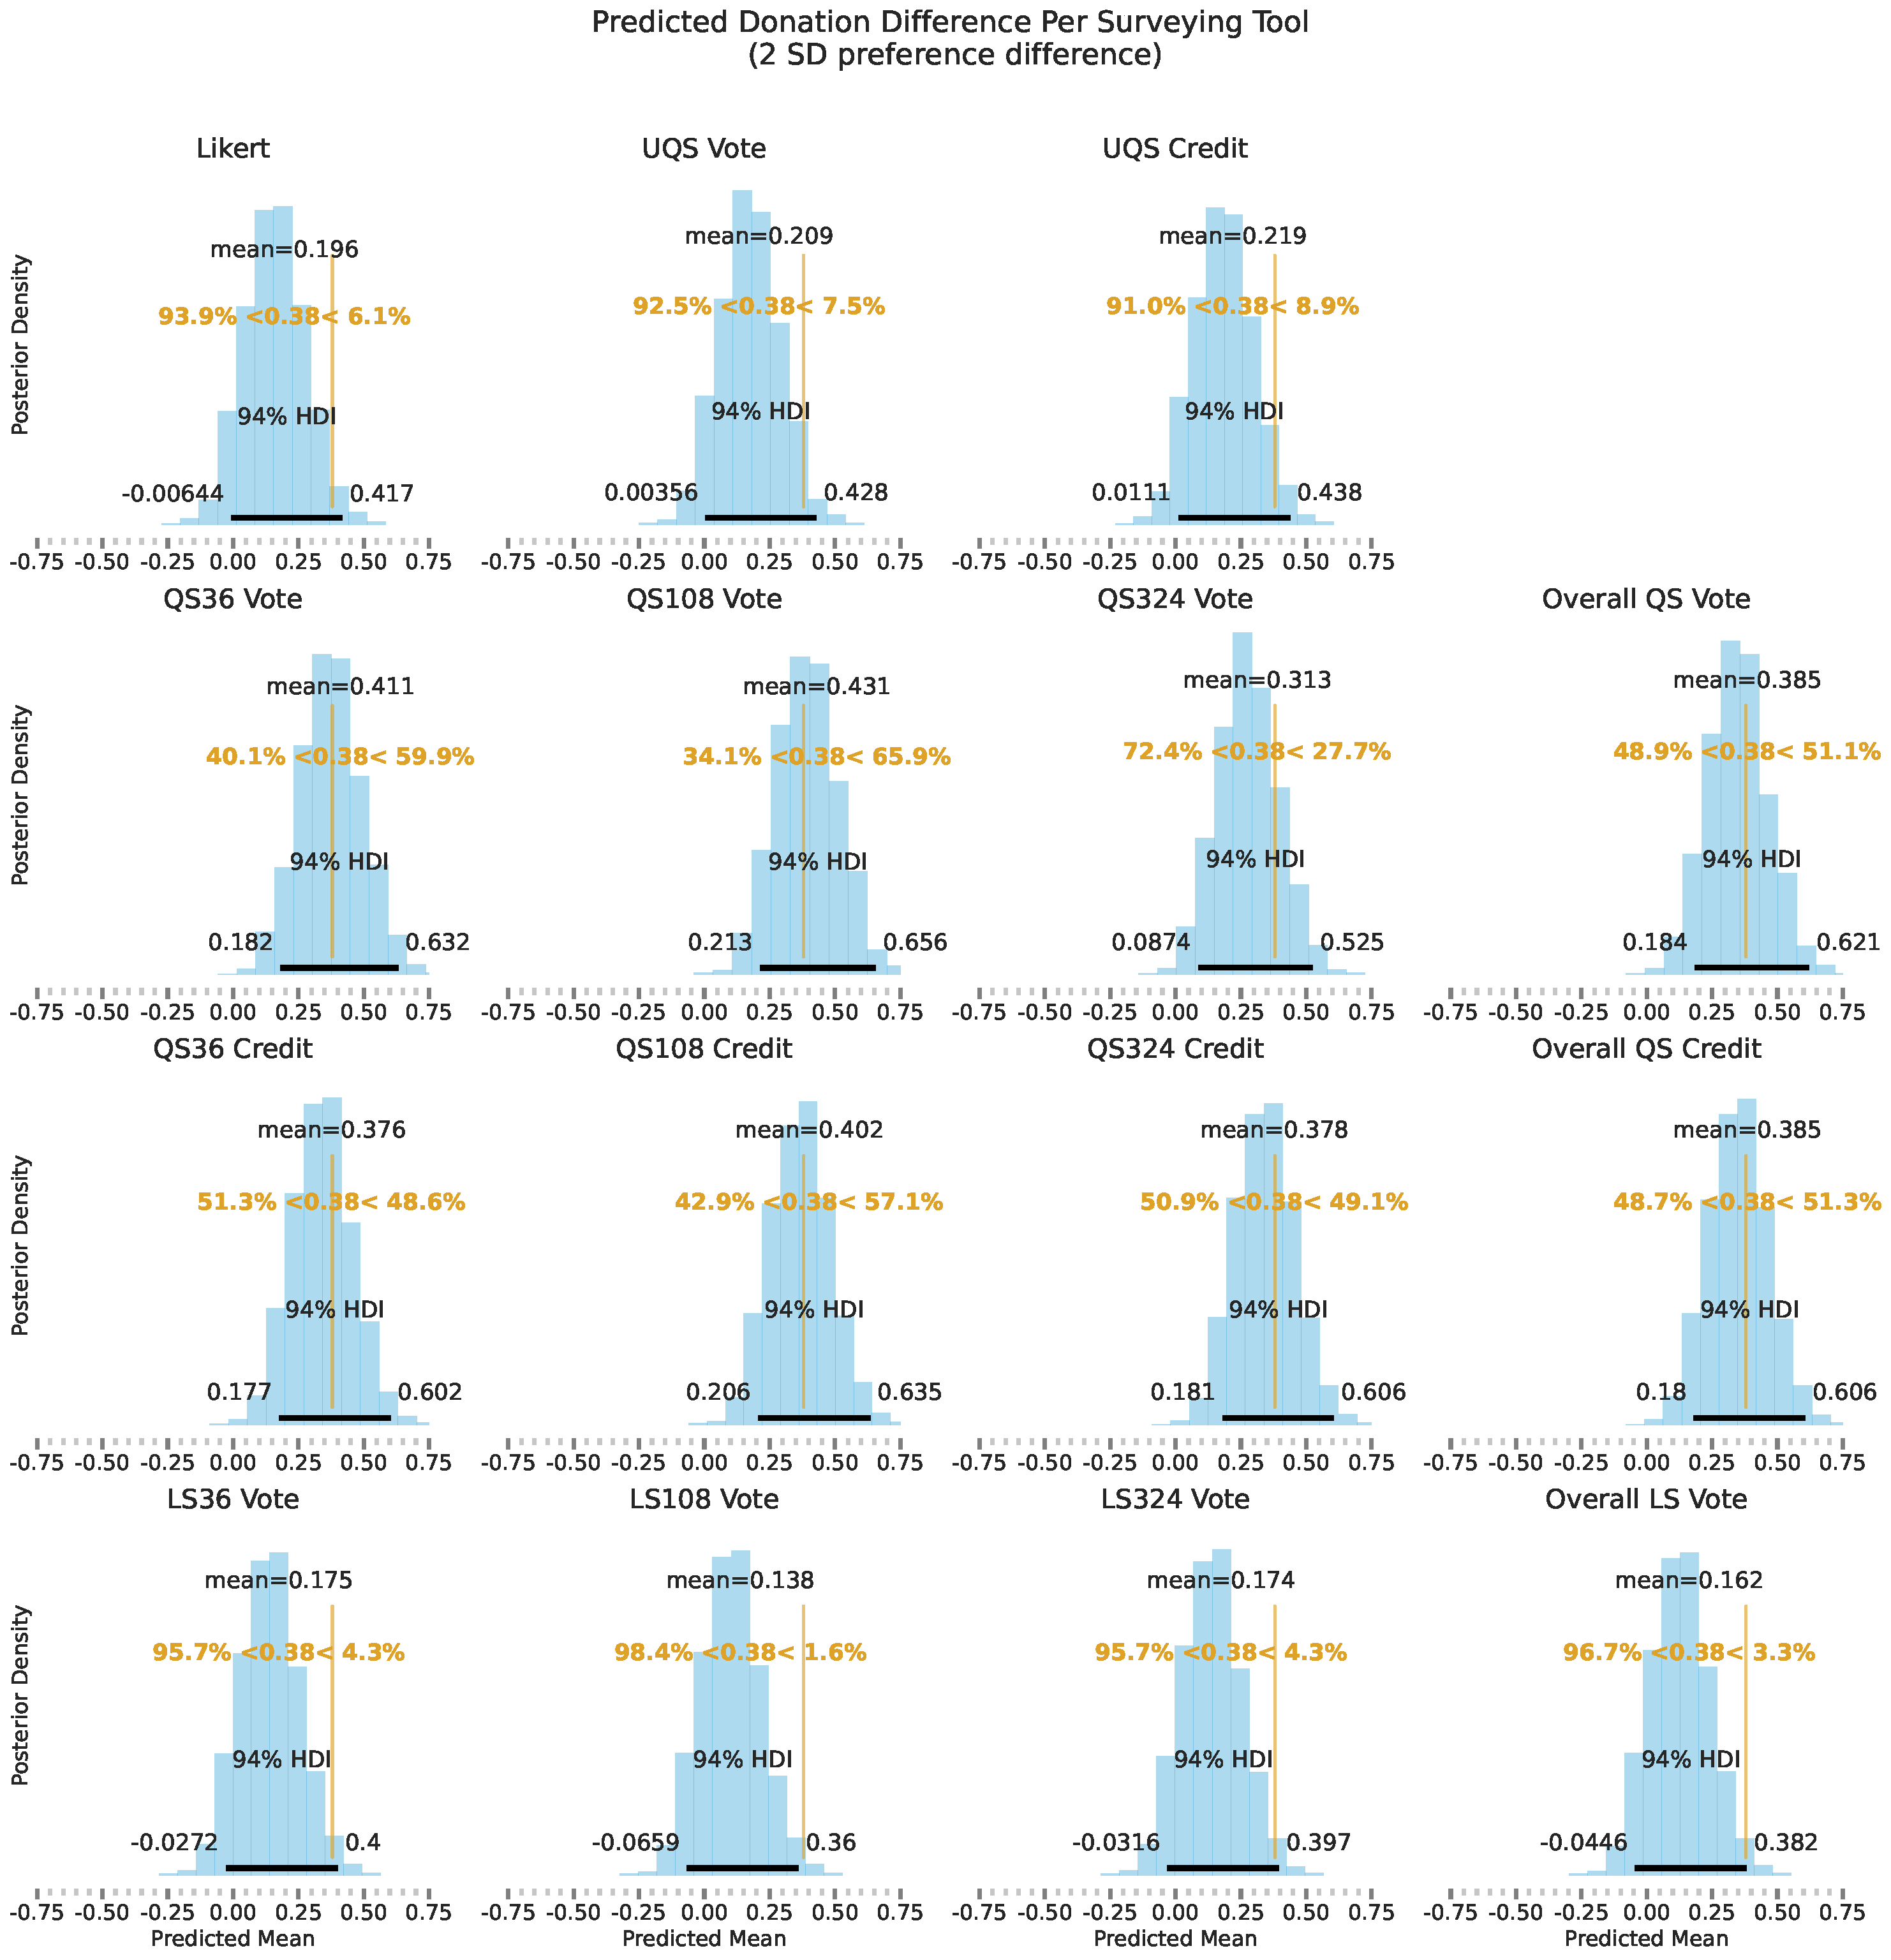
\includegraphics[width=\textwidth]{content/image/intensity_2sd.pdf}
    \caption{
    The posterior predictive distributions of donation differences for various surveying tools, assuming that the surveyed preference difference between two options is 2 standard deviations (SD) within our dataset's all pairwise differences. The x-axis displays predicted mean donation differences, while the y-axis represents posterior density, indicating the probability of various predicted mean donation differences occurring. The region indicated by the bolded black line represents the 94\% Highest Density Interval (HDI), providing the most credible range for the predicted donation difference. A vertical gold line at 0.38 reflects the ``perfect'' donation value corresponding to a 2 SD-surveyed preference difference. In this plot, aside from QS (votes and credit), other surveying tools produced donation predictions that fell short of the 0.38 threshold, suggesting that these tools overly expressed preference intensity rather than accurately capturing it.~\textbf{Main takeaway:} QS is capable of capturing the intensity of medium-sized (2 SD) preference differences between options accurately.
    }
    \label{fig:donation_posterior}
\end{figure*}


\textbf{Results interpretation:} With the fitted intensity model, we calculate the posterior predictive distribution of the mean of donation differences ($\mu_{\Delta_{\text{Predicted Donation}}}$), given a preference difference intensity between any two options elicited by a survey tool ($\Delta_{\text{Survey}}$). Three such distributions are constructed for each survey tool, one for a small, medium, and large preference difference elicited by the tool respectively (i.e., $\Delta_{\text{Survey}}$ = 0.19, 0.38, 0.57, corresponding to $median(\Delta_{\text{Survey}})+k \times std(\Delta_{\text{Survey}})$, where $k=1, 2, 3$). We then perform two comparison tasks using these posterior distributions of $\mu_{\Delta_{\text{Predicted Donation}}}$. 

First, we evaluate if predicted normalized donation differences $\Delta_{\text{Predicted Donation}}$ significantly differ from the ``perfect'' predicted donation difference ($\Delta_{\text{Donation Ref}}$). A predicted normalized donation difference between two options is ``perfect'' when it equals the normalized difference between the preferences elicited by the survey tool ($\Delta_{\text{Donation Ref}} = \Delta_{\text{Survey}}$). When $\Delta_{\text{Predicted Donation}} < \Delta_{\text{Donation Ref}}$, it means that our participants donated less to their preferred option than they said they would on the survey (relative to the less-preferred option), and vice-versa. We conclude that a survey tool failed to reflect a given preference difference intensity well when the 94\% Highest Posterior Density Interval (HPDI) of the distribution of $\mu_{\Delta_{\text{Predicted Donation}}}$ does not include $\Delta_{\text{Donation Ref}}$. 

Second, we compare the posterior distributions of $\mu_{\Delta_{\text{Predicted Donation}}}$ between survey conditions for the same $\Delta_{\text{Survey}}$. Such comparisons provide insights into how a survey tool performs relative to another. We construct the posterior distribution of Cohen's d to quantify the difference between the $\mu_{\Delta_{\text{Predicted Donation}}}$ of a pair of survey conditions. We report that a survey tool's ability to reflect a preference intensity differs from another when the 94\% HPDI of the Cohen's d distribution excludes zero. 

%\textbf{Small  in all tested survey tools predicted $\Delta_{\text{Predicted Donation}}$ well.}
Small differences in survey responses~($\Delta_{\text{Survey}}$) reliably predicted differences in donation behavior~($\Delta_{\text{Predicted Donation}}$) across all conditions. Among them, Likert, UQS vote, UQS credit, and LS results aligned best with donation differences ($\mu_{\Delta_{\text{Predicted Donation}}}$ = 0.15, 0.17, 0.18, 0.15, respectively; $\Delta_{\text{Donation Ref}}$ = 0.19). When participants expressed a small difference in QS vote and credit between two options, they expressed larger differences in donations (mean of $\mu_{\Delta_{\text{Predicted Donation}}}$ = 0.29, 0.26, respectively). But their donation differences did not differ significantly from the ``perfect'' difference ($\Delta_{\text{Donation Ref}}$ = 0.19).

\textbf{As $\Delta_{\text{Survey}}$ increased to medium and large sizes, only those elicited by QS (both vote and credit, regardless of the budget size) were well-reflected in the corresponding donation differences.} For instance, Figure~\ref{fig:donation_posterior} shows that when QS vote and credit $\Delta_{\text{Survey}} = 0.38$ (medium difference), the mean of $\mu_{\Delta_{\text{Predicted Donation}}} = 0.39$ (94\% HPDI for QS vote = [0.18, 0.62], for QS credit = [0.18, 0.61]). \textbf{Results from QS aligned significantly better with donation results than those from the Likert scale with a medium to large effect size}\footnote{Cohen's d = 0.2, 0.5, 0.8 corresponds to a small, medium, and large effect size, respectively}. Moreover, QS's advantage over the Likert scale increased with $\Delta_{\text{Survey}}$, as shown in Figure~\ref{fig:comparison}. Using the donation prediction accuracy of QS credit vs. Likert scale as an example, the mean Cohen's d increases from 0.71 to 0.99 when $\Delta_{\text{Survey}}$ changes from medium (Cohen's d 94\% HPDI = [0.62, 0.81]) to large (Cohen's d 94\% HPDI = [0.89, 1.09]).

\textbf{On the other hand, for medium and large $\Delta_{\text{Survey}}$, UQS (i.e., QS without a budget) predicted donation difference similarly to the Likert scale, hence significantly worse than QS. Furthermore, LS with various budget sizes (i.e., QS without the quadratic cost) performed worse than Likert and UQS with a small effect size.} When participants conveyed a medium-sized or larger preference difference between two options in Likert, UQS, or LS, they expressed a weaker difference in donations. A large $\Delta_{\text{Survey}}$ in Likert, UQS, and LS, for instance, predicted a mean $\mu_{\Delta_{\text{Predicted Donation}}}$ of 0.25, 0.25, and 0.17 respectively, far lower than the ideal difference ($\Delta_{\text{Donation Ref}}$ = 0.57).
\section{Discussion}
\label{sec:discussion}
This section addresses the research questions, interprets findings, and offers practical recommendations.

\subsection{QS's effectiveness and its dual components}
We evaluated the effectiveness of QS in capturing pairwise preferences (RQ1) and whether both the quadratic cost function and budget constraint are necessary (RQ2). Results indicate that QS, whether analyzed through votes or costs, consistently outperforms Likert scale surveys in recovering ordinal rankings and preference intervals—especially when resources are constrained. Moreover, QS shows increasing advantages as preference gaps widen, capturing intensities with greater accuracy over other methods.

Results suggest that both the quadratic cost function and the fixed budget constraint are essential to QS’s effectiveness. Performance drops significantly when either is removed, as observed in LS and UQS (see~\Cref{sec:result_2}). This gap between LS and QS requires further investigation, as discussed in the following subsections.

%Rather than simplifying the mechanism, design efforts should prioritize interfaces that support participant engagement. 



% (e.g., scaffolding for preference construction~\cite{chengOrganizeThenVote2025})


\begin{figure*}[h]
    \centering
    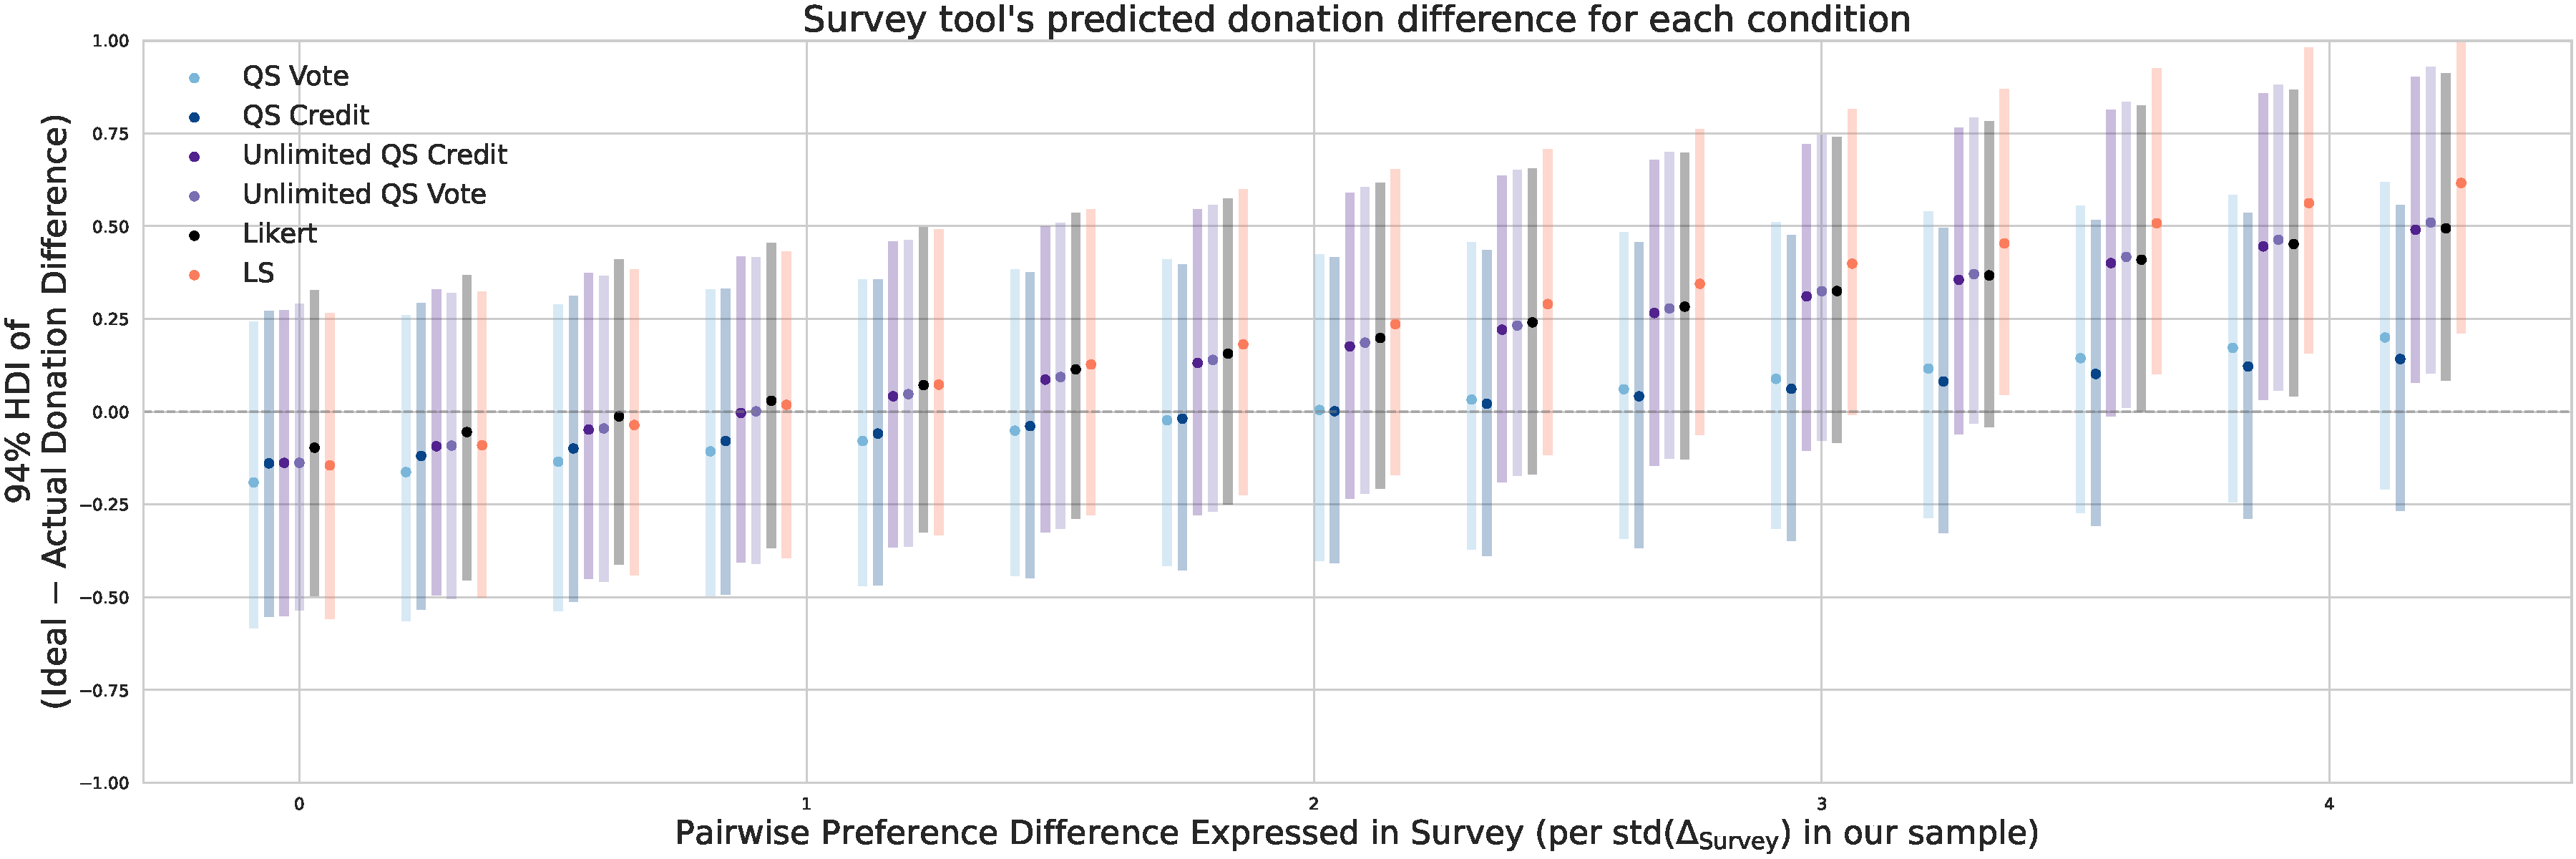
\includegraphics[width=\textwidth]{content/image/posterior_predictive_cumulative.pdf}
    \caption[]{Differences between survey-reported preferences and actual donation behaviors across survey tools. Dots represent mean normalized differences, with bars showing the 94\% Highest Density Interval (HDI). The horizontal line at 0 indicates perfect alignment; values above represent overstated preferences. QS Vote and QS Credit consistently show close alignment even as actual behavioral differences increase, while Likert, LS, and Unlimited QS increasingly deviate at larger differences. \textbf{Takeaway}: QS methods (Vote and Credit) better capture participants' actual preference intervals, especially as intensity differences grow.}
    \label{fig:comparison}
\end{figure*}

\subsection{Mechanisms underlying QS's effectiveness}
This subsection explores the plausible mechanisms underlying QS's effectiveness. While our results replicate and extend the observed advantage of QS over Likert scale surveys~\cite{chengCanShowWhat2021}, we focus this subsection on two mechanisms: (1) how the quadratic cost function aligns preferences with behavior, and (2) how budget constraints shape expression. We examine these mechanisms using LS and UQS results.

\subsubsection{Quadratic cost function corrects perception distortion and bias in response strengths}
As discussed in~\Cref{sec:interval_measures}, QS credits and votes remain aligned with participants' revealed behaviors across varying levels of preference strength. In contrast, our model shows increased exaggeration in LS and Likert scale survey results as the pairwise donation difference widens (see~\Cref{fig:comparison}). We identify two plausible explanations.

\paragraph{Unequal~\textit{perceived} `preference units'}
We define a 'preference unit' as the incremental amount a participant uses to express additional preference (e.g., an extra vote, extra credits spent, or an extra level on a Likert scale). Our results indicate that LS participants perceive successive preference units as representing smaller incremental differences in strength. This pattern aligns with the Law of Diminishing Marginal Utility in economics~\cite{gossen1983laws, kahnemanProspectTheoryAnalysis1979}, which states that each additional unit of consumption yields less utility than the one before. Thus, survey respondents allocate more preference units to express their intended preferences.

Even if participants do not explicitly interpret preference units in monetary terms, psychophysics offers similar concepts. According to the Weber-Fechner law~\cite{dehaeneNeuralBasisWeber2003, kruegerReconcilingFechnerStevens1989}, the just noticeable difference between stimuli is proportional to the baseline stimulus intensity. As the marginal difference between options appears to shrink, participants may feel their previous input was insufficient and overcorrect as a result. Early CSS validation by~\citet{dudekValidityPointAssignmentProcedure1957} cautioned that participants may misjudge how well their numerical input reflects their subjective attitudes. Interestingly, Fechner's law~\cite{kruegerReconcilingFechnerStevens1989} describes perception as following a logarithmic curve, which conceptually aligns with the quadratic cost structure in QS. In QS, the rising cost of additional votes may have corrected participants' diminishing perceptual increments, helping to mitigate exaggerations in expressed preferences stemming from participants' perceptual biases.

\paragraph{Extreme response bias}
Another plausible explanation involves the large decision space and the ease of expressing extreme opinions offered by LS. With the same budget size, participants face a wider array of allocation choices when votes incur a linear cost than a quadratic cost (e.g., 324 choices in LS162 vs. 25 choices in QS162 on an option). The psychology literature suggests that cognitive overload leads to satisficing~\cite{schwartzMaximizingSatisficingHappiness2002, iyengarWhenChoiceDemotivating2000}, where individuals settle for sufficient rather than optimal choices by relying on heuristics. As the allocated budget increased, participants increasingly underutilized their budgets, a pattern consistent with satisficing behavior~(\Cref{fig:credit_usage_descending}). With a satisficing mindset, rather than carefully weighing and quantifying the differences between options, participants may resort to exaggerating responses to signal distinctions between choices. While this exaggeration strategy is possible with both LS and QS, it was discouraged by the quadratic cost structure in QS. The quadratic cost function imposes increasing costs for each additional vote, which makes people think twice before expressing strong opinions. In LS, on the contrary, it does not cost much to exaggerate preferences since each vote carries equal weight. In summary, the quadratic cost structure in QS may have reduced the occurrences of exaggerated responses by alleviating cognitive load and imposing a higher cost to expressing extreme opinions.
% which lets individuals redistribute credits freely, since each vote carries equal weight. As the LS budget increases, the space of possible allocations grows rapidly. Consider LS18 and QS324, which both permit up to 18 votes~\footnote{Assuming all credits are allotted to a single option, 324 credits allows at most 18 votes which is equivalent to LS18.}; however, in QS, casting 18 votes incurs a significantly higher cost.  sharply narrowing the decision space and discouraging exaggerated responses.

\begin{figure}[ht]
  \centering

  \begin{minipage}[t]{0.48\textwidth}
    \centering
    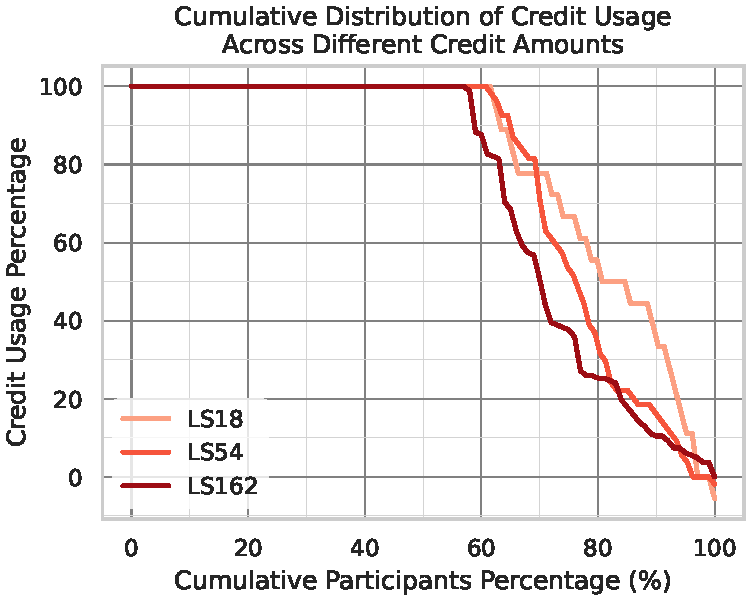
\includegraphics[width=\textwidth]{content/image/cumulative_distribution_credit_usage.pdf}
    \caption[]{
    Percentage of participants who fully utilized their credits across budget levels. As budgets increase, cumulative usage drops off more steeply.
    \textbf{Takeaway:} Higher budgets lead to earlier and more widespread underutilization of credits.
    }   
    \label{fig:credit_usage_descending}
  \end{minipage}
  \hfill
  \begin{minipage}[t]{0.48\textwidth}
    \centering
    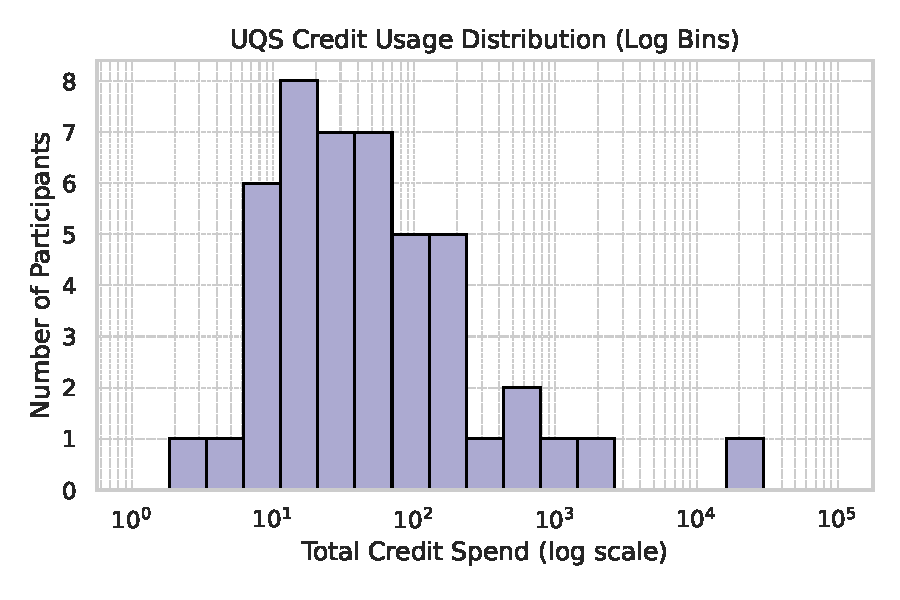
\includegraphics[width=\textwidth]{content/image/uqs_credit_usage_distribution_logbins.pdf}
    \caption[]{The credit usage distribution for UQS participants. The credit usage follows a long tail. Without an anchor, less than half of participants spend more than 38 credits across 9 options. \textbf{Takeaway:} Participants did not put in enough effort to use as many credits as needed to express nuanced differences between option preferences.}
    \label{fig:uqs_usage}
  \end{minipage}

\end{figure}


\subsubsection{The quadratic cost function reduces the cognitive burden influencing pairwise rankings}
This expanded decision space may have also undermined LS's ability to preserve pairwise rankings that are consistent with participants' opinions. The linear cost in LS increases the number of possible allocation outcomes compared to QS with the same budget size, raising the cognitive demand required to maintain consistent relative preferences. In contrast, QS's quadratic cost structure progressively narrows this decision space, easing the cognitive burden and facilitating more consistent preference rankings. This cognitive burden likely contributes to noisier and more inconsistent pairwise rankings. %This likely contributes to noisier and more inconsistent survey pairwise rankings. When a participant allocates $x$ votes to one option, they face a wide range of subsequent options (e.g., $x+1$ to the remaining budget) to express stronger preferences elsewhere. 

\subsubsection{The role of Budget: Anchor and a Sense of Scarcity}
UQS performs similarly to LS, likely due to two key factors. First, without a fixed budget, participants face unlimited allocation options, eliminating clear opportunity costs and tradeoffs. This can result in more extreme allocations or exaggerated expressions (e.g., one participant allocated 105 votes to a single option). Second, without a budget constraint, participants lack a stable reference for a 'preference unit,' since the meaning or weight of each additional vote shifted with each allocation. This undermines anchoring~\cite{daniel2017thinking, tverskyJudgmentUncertaintyHeuristics1974}, often necessary for initiating preference construction~\cite{lichtensteinConstructionPreference2006}, and further expands the decision space. We observe that less than half of the participants spend more than 38 credits, followed by a long tail of credit usage (\Cref{fig:uqs_usage}), possibly due to cognitive overload or because they felt further input was unnecessary. This behavior constrained the expansive decision space, suggesting that budget limits may help regulate expressive intensity.

\paragraph{In summary,} QS's quadratic cost function helps mitigate distortions caused by perceptual biases and choice overload, particularly when participants express large differences between options. The fixed budget constraint anchors participants' interpretations of preference units and limits the decision space, thereby reducing cognitive load and supporting more accurate expression.

Together, these mechanisms likely explain why QS aligns more closely with participants' behavioral outcomes than the alternatives. While each mechanism is grounded in prior literature and supported by our findings, their interaction remains unclear. Perceptual distortion, overload, and anchoring may be interdependent rather than isolated effects. Future research should investigate how participants' internally valued preferences map onto their expressed responses in QS. Cognitive interviews aimed at constructing mental models could reveal how participants interpret budget constraints, cost structures, and manage preference tradeoffs during preference construction.

\subsection{Takeaways for QS practitioners}
Our findings offer practical implications for practitioners using QS to elicit preferences in collective intelligence settings:

\paragraph{Balancing simplicity and accuracy for basic ranking tasks}
Likert scale surveys may suffice for simple rankings that do not require aggregation, given their simplicity. While QS still yields slightly better alignment with behavioral outcomes, the added complexity may not be justified in low-stakes or ordinal-only contexts.

\paragraph{QS excels in capturing preference intensity and enabling aggregation}
QS is particularly effective for capturing nuanced differences in preference strength across competing options and aggregating those preferences across individuals. Our results demonstrate that QS significantly outperforms traditional methods in capturing preference intensities and enabling aggregation.

\paragraph{Do not compromise the QS mechanism}
Both the quadratic cost function and the budget constraint are essential for QS to function effectively. Removing either component (as in LS or UQS) substantially reduces performance. Since these features introduce cognitive load, it is essential to design usable interfaces that support participants' preference construction process.

\paragraph{Credit budget matters less, but a medium range is recommended}
Although we observed no statistically significant differences among QS36, QS108, and QS324, Bayesian analysis consistently favored QS108 for stable, balanced outcomes. Thus, practitioners are advised to scale the credit budget to the power of 1.5 relative to the number of options ($O(k^{1.5})$ as defined by prior research~\cite{chengCanShowWhat2021}.

\section{Limitations and Future work}
\label{sec:limitations}

\paragraph{Limitations of donation-based preference elicitation}
Behavioral donation tasks are widely used in prior research~\cite{xiao2019should, gendall2010effect, benz2008people, chengCanShowWhat2021} to approximate ``true preferences'' through real-stakes decisions for survey validation. While the donation task in this study was adapted from prior designs to ensure incentive compatibility and behavioral realism, not all preferences are naturally expressed through monetary contributions. Participants' mental models, shaped by donation amounts, prior giving, or personal motivations, may differ from those guiding their responses to survey instruments. Moreover, although charitable donations offer incentive-aligned behavior, the domain involves distinct social and motivational factors that may not generalize to other allocation contexts. Governmental resource allocation, for instance, includes political accountability, public transparency, and long-term planning considerations. Future field studies applying QS in public decision-making settings could further assess its generalizability.

\paragraph{Future work: comparing QS with other forced-choice methods}
The limited performance of LS highlights the need for future comparative studies between QS and other forced-choice preference elicitation tools, such as KS and conjoint analysis. These methods rely on different constraints and mechanisms to reveal preference intensity. Comparing them across decision contexts and preference distributions would help practitioners identify the most appropriate tools. Future evaluations should consider elicitation accuracy, cognitive load, and user experience.

\section{Conclusion}
This work advances the understanding of QS by examining how its embedded constraints shape expressed preferences and participant behavior. Through controlled comparisons with LS and UQS, we isolate the effects of the quadratic cost function and budget constraint on alignment with behavioral outcomes. QS performs well only when both components are present; removing either weakens its ability to capture accurate rankings and intensities, particularly as preference gaps grow. These findings support QS as a valuable tool for eliciting relative preferences in resource-constrained settings. They also highlight the need to better understand how individuals interpret votes, budgets, and effort when forming preferences. Future work should investigate these mental models to inform more effective and usable QS designs.
\begin{acks}
We thank the study participants for their time and contributions. We are also grateful to Dr. Michel Regenwetter, Vinay Koshy, James Eschrich, Andrew Chen, and Aditya Karan for their valuable feedback. This work would not have been possible without the support of peers from the Social Spaces and Crowd Dynamics Lab. Additional thanks to Hsin-Ni Yu and Chi-Chun Huang. This research was partially supported by the Center for Just Infrastructures.
\end{acks}




% \printbibliography
\bibliography{tcheng, references}

% TC:ignore
% \appendix

% % Interface Design Appendix
% \section{Interface Design}
\section{Interface design process}\label{apdx:design}
In this section, we outline the design process leading to our final interface.% As mentioned in the paper, our design iteration began from existing QV applications in the wild.

\begin{figure}[H]
    \centering
    % First subfigure
    \begin{subfigure}[b]{\linewidth}
        \centering
        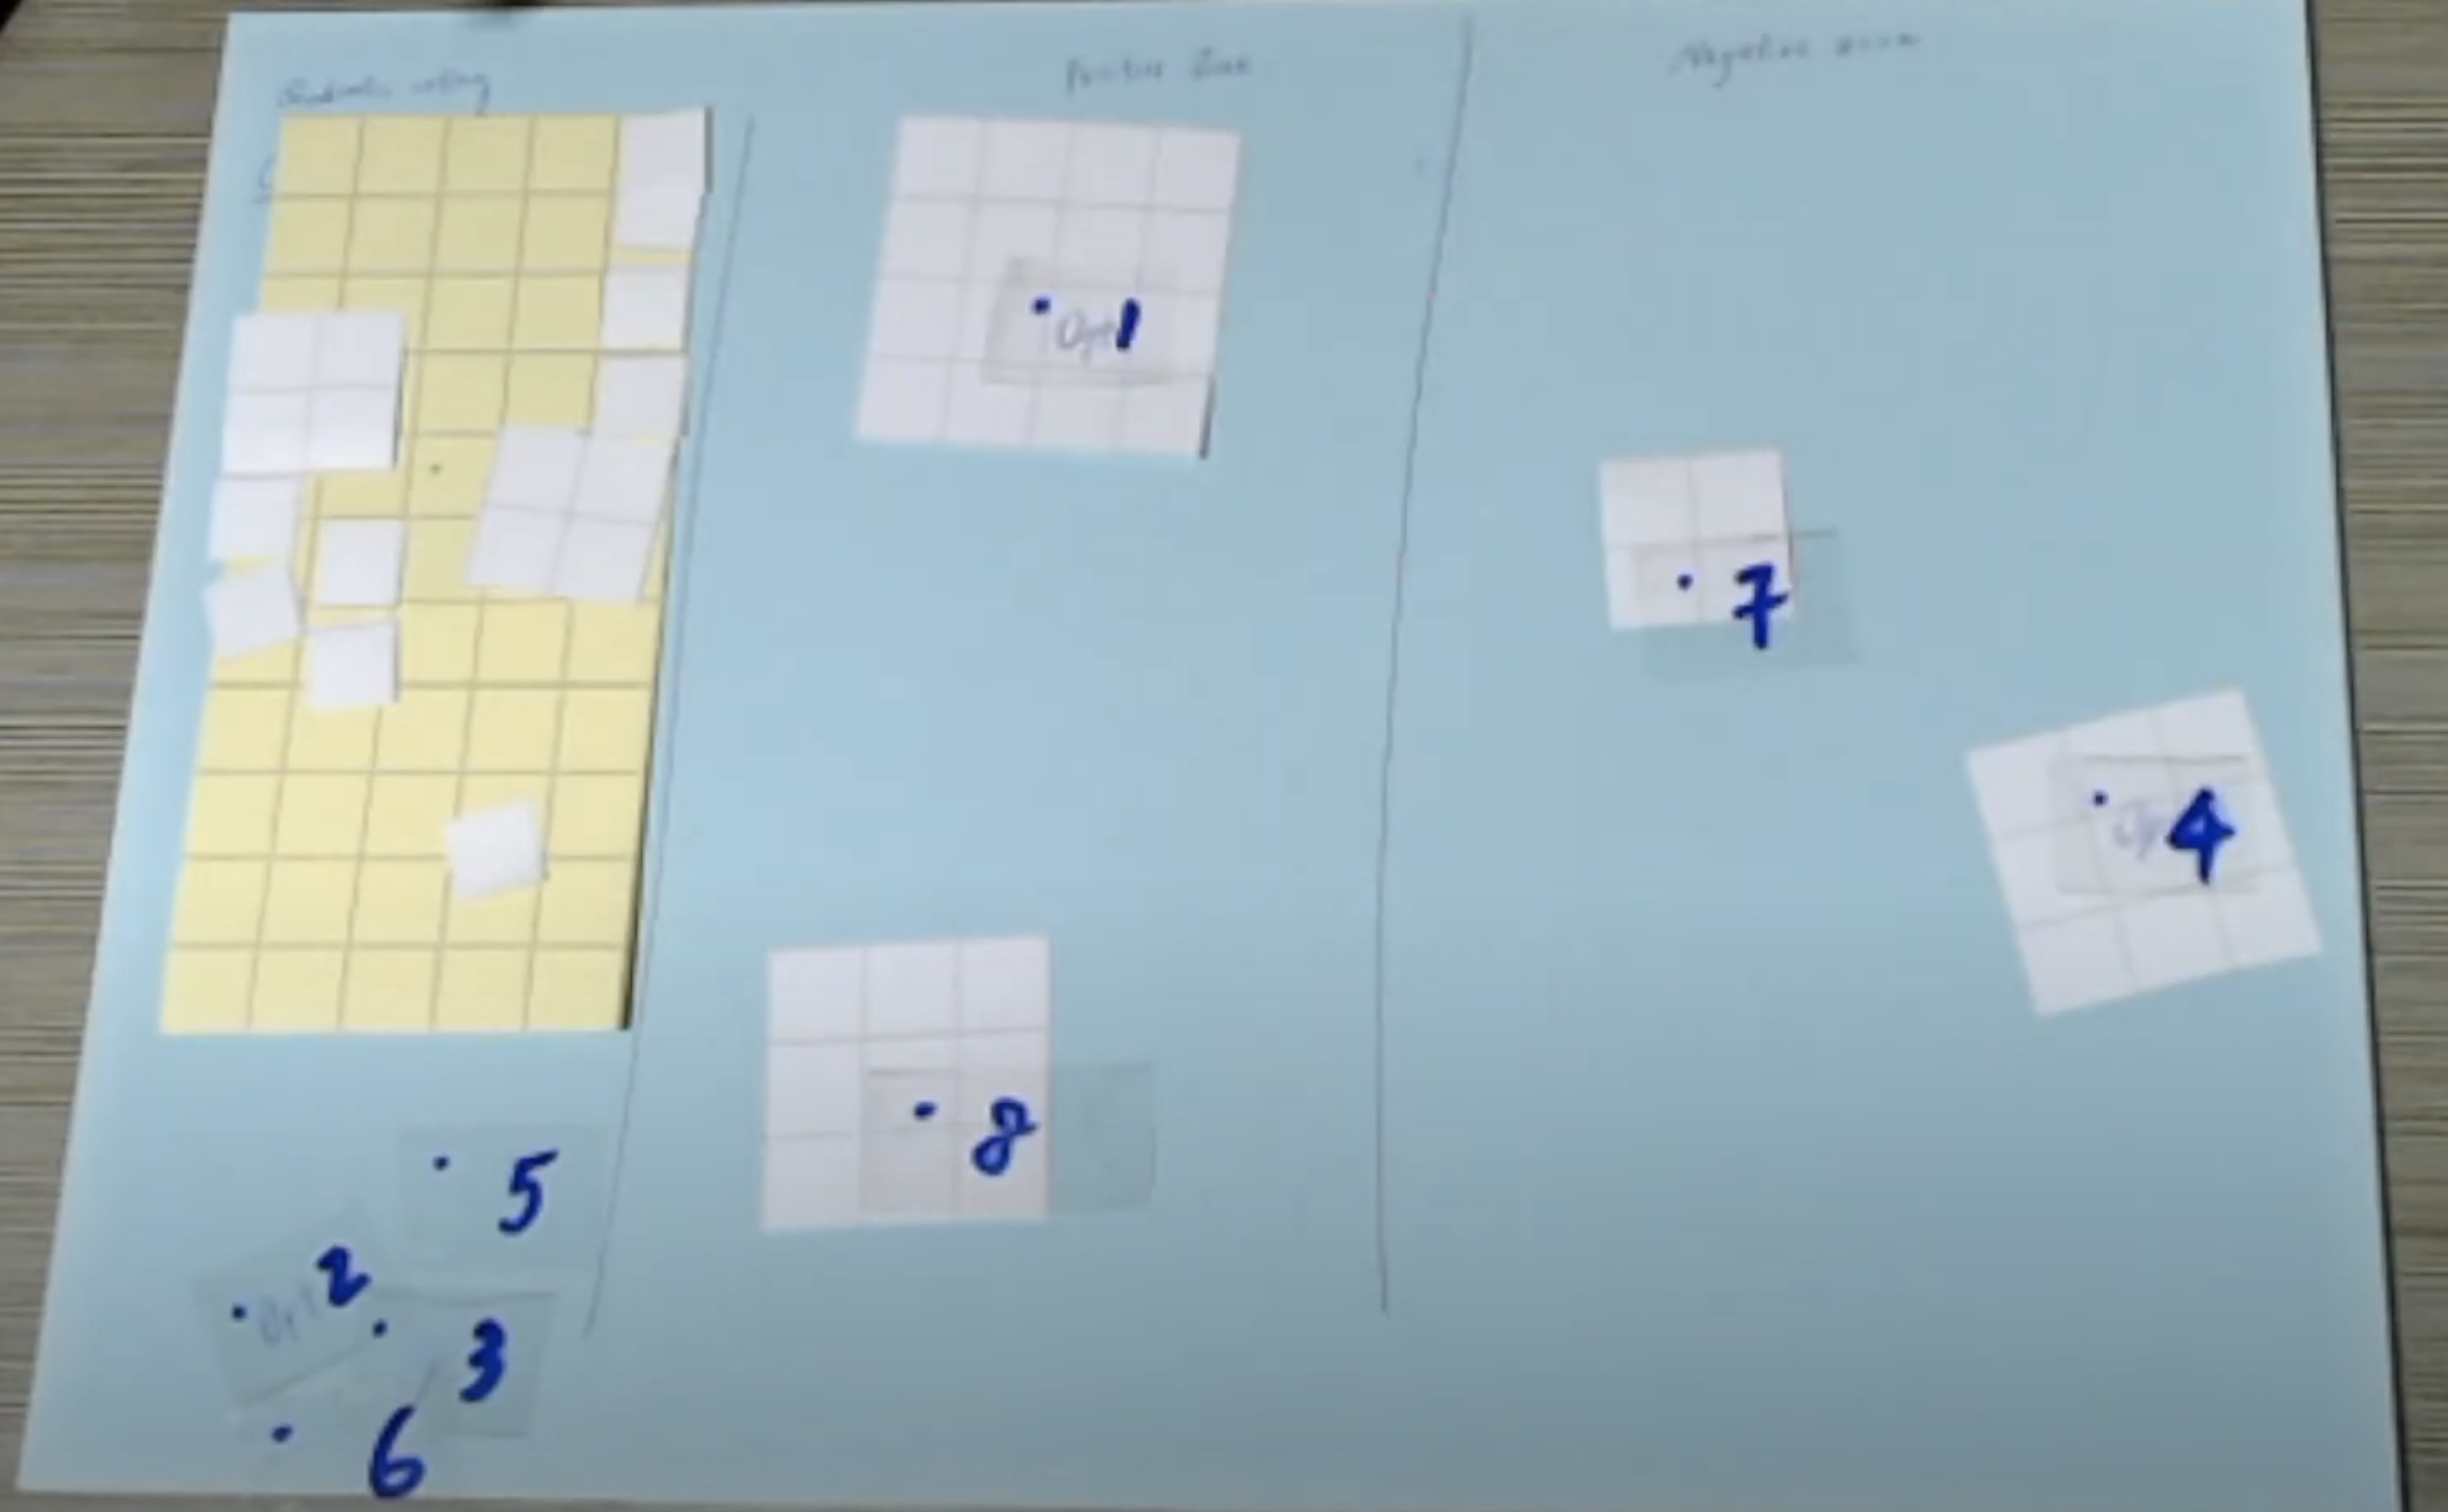
\includegraphics[width=0.9\linewidth]{content/image/prototypes/1.2_paper_qv_single.png}
        \caption{In this paper prototype, issues are denoted by different numbers that appear on mouseover. Pretest respondents can move options anywhere in the two sections of the interface, one denoting positive and one negative. The blocks represent the cost for each option, with no indication of the number of current votes. The credits are shown in the yellow box on the left.}
        \Description{An image of a paper prototype showing different sections for respondents to interact with. On the left side, a yellow grid contains small white squares, some of which are stacked and scattered outside the grid. The middle section labeled "Positive Zone" contains a large white square with a grid, labeled "Opt 1". The right section, labeled "Negative Zone," contains two white squares, each with grids, labeled with numbers 7 and 4. Additional small white squares labeled with numbers 2, 3, 5, 6, and 8 are positioned around the prototype. The yellow box on the left represents available credits.}
        \label{fig:horizontal_paper}
    \end{subfigure}

    \vspace{1em} % Adjusts vertical spacing between figures

    % Second subfigure
    \begin{subfigure}[b]{\linewidth}
        \centering
        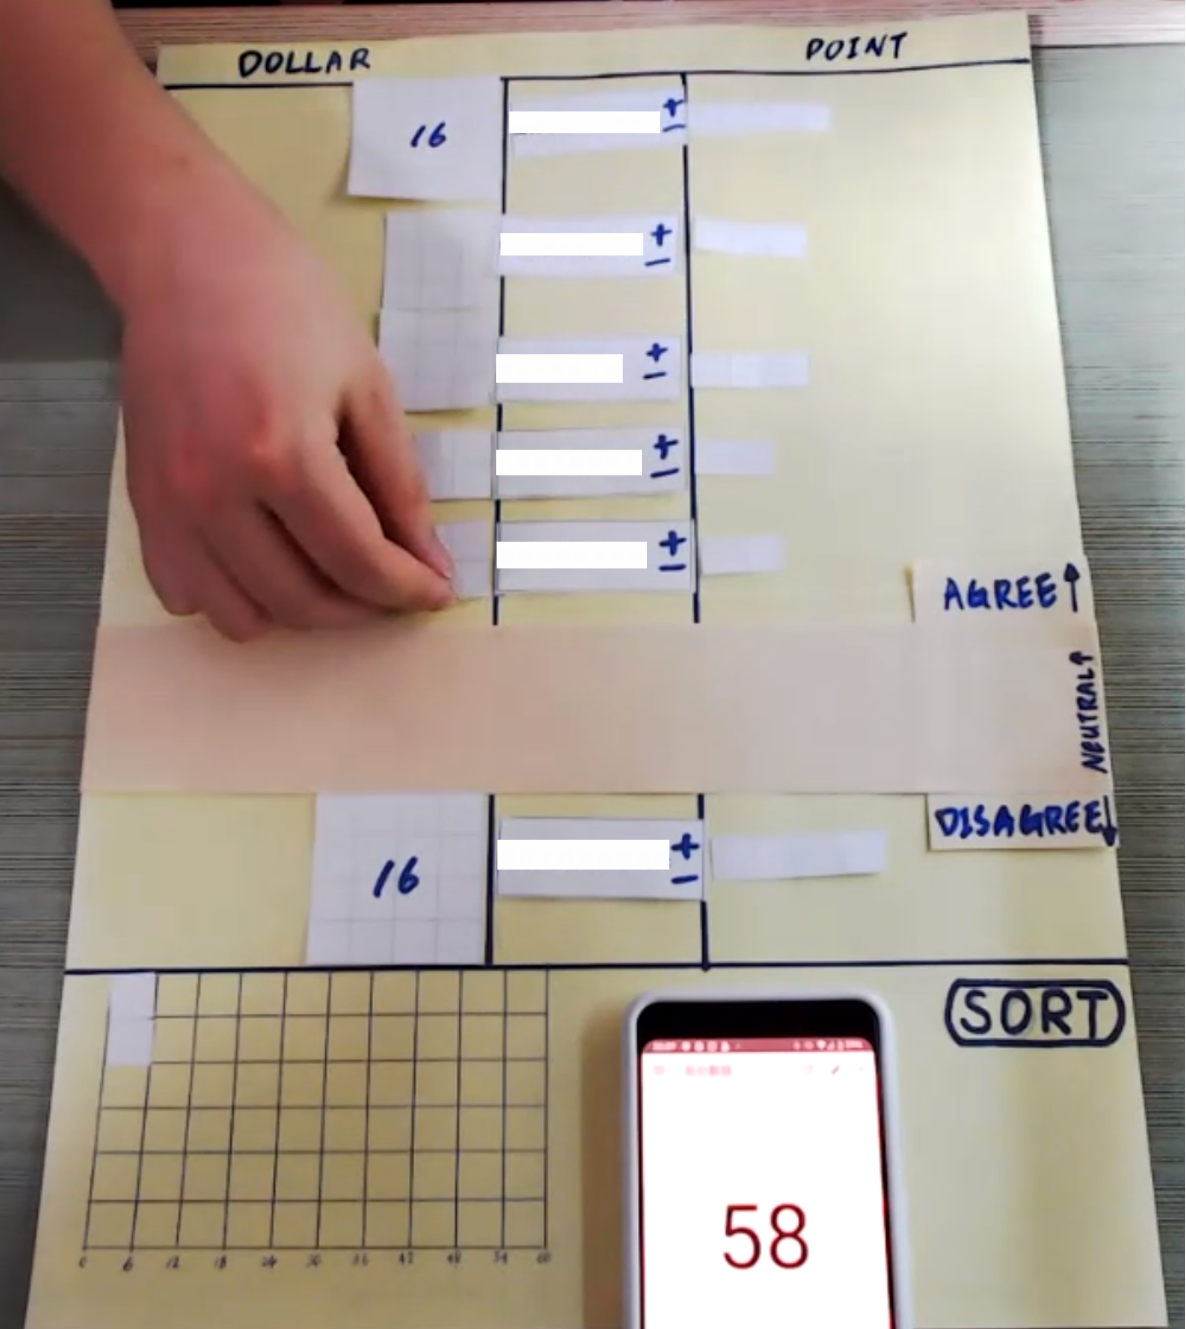
\includegraphics[width=0.77\linewidth]{content/image/prototypes/1_paper_qv_single.png}
        \caption{This paper prototype separates the positive and negative areas with a 'band' at the center. Undecided options are placed inside this band. The cost and the votes on both sides of the interface are denoted by small blocks. The budget is shown in the yellow box below the interface with a numerical counter.}
        \Description{A paper prototype interface where a person's hand is interacting with blocks. The prototype separates positive and negative areas using a wide horizontal band in the center, which holds undecided options. On the left side of the band, a column labeled "Dollar" shows a block marked with the number 16. On the right side, under a column labeled "Point," several rows have small blocks with plus and minus signs, indicating positive and negative areas. At the bottom left, a yellow box with a grid shows the available budget, marked with the number 16. A smartphone in the bottom right corner displays the number 58.}
        \label{fig:vertical_paper}
    \end{subfigure}

    \caption{Initial paper prototypes designed for QS interface.}
    \Description{This figure contains two subfigures showing two different paper prototypes.}
    \label{fig:qv_paper}
\end{figure}

\subsection{Prototype 1: Ranking-Vote}
Our first prototype emerged after various paper prototypes, such as those shown in~\Cref{fig:qv_paper}. Through pre-testing, we observed that participants engaging with QS needed interface support for organizing options and managing their credits. In this study, we decided to focus on the former.

Since participants needed to position options within the interface, and the end result formed a ranked list, we tested whether ranking options before voting would help establish an individual's relative preferences in Prototype 1 (~\Cref{fig:qv_rank}). This prototype allowed respondents to reposition options before voting. However, pre-test respondents rarely moved the options and questioned the necessity of a full ranking, as it did not influence their QS submission. Additionally, many were unaware that the options were draggable.These findings suggest that a full ranking is unnecessary for establishing relative preferences. Therefore, we decided to ask respondents to select a subset of options rather than requiring a full ranking of all options.

\begin{figure}[H]
    \centering
    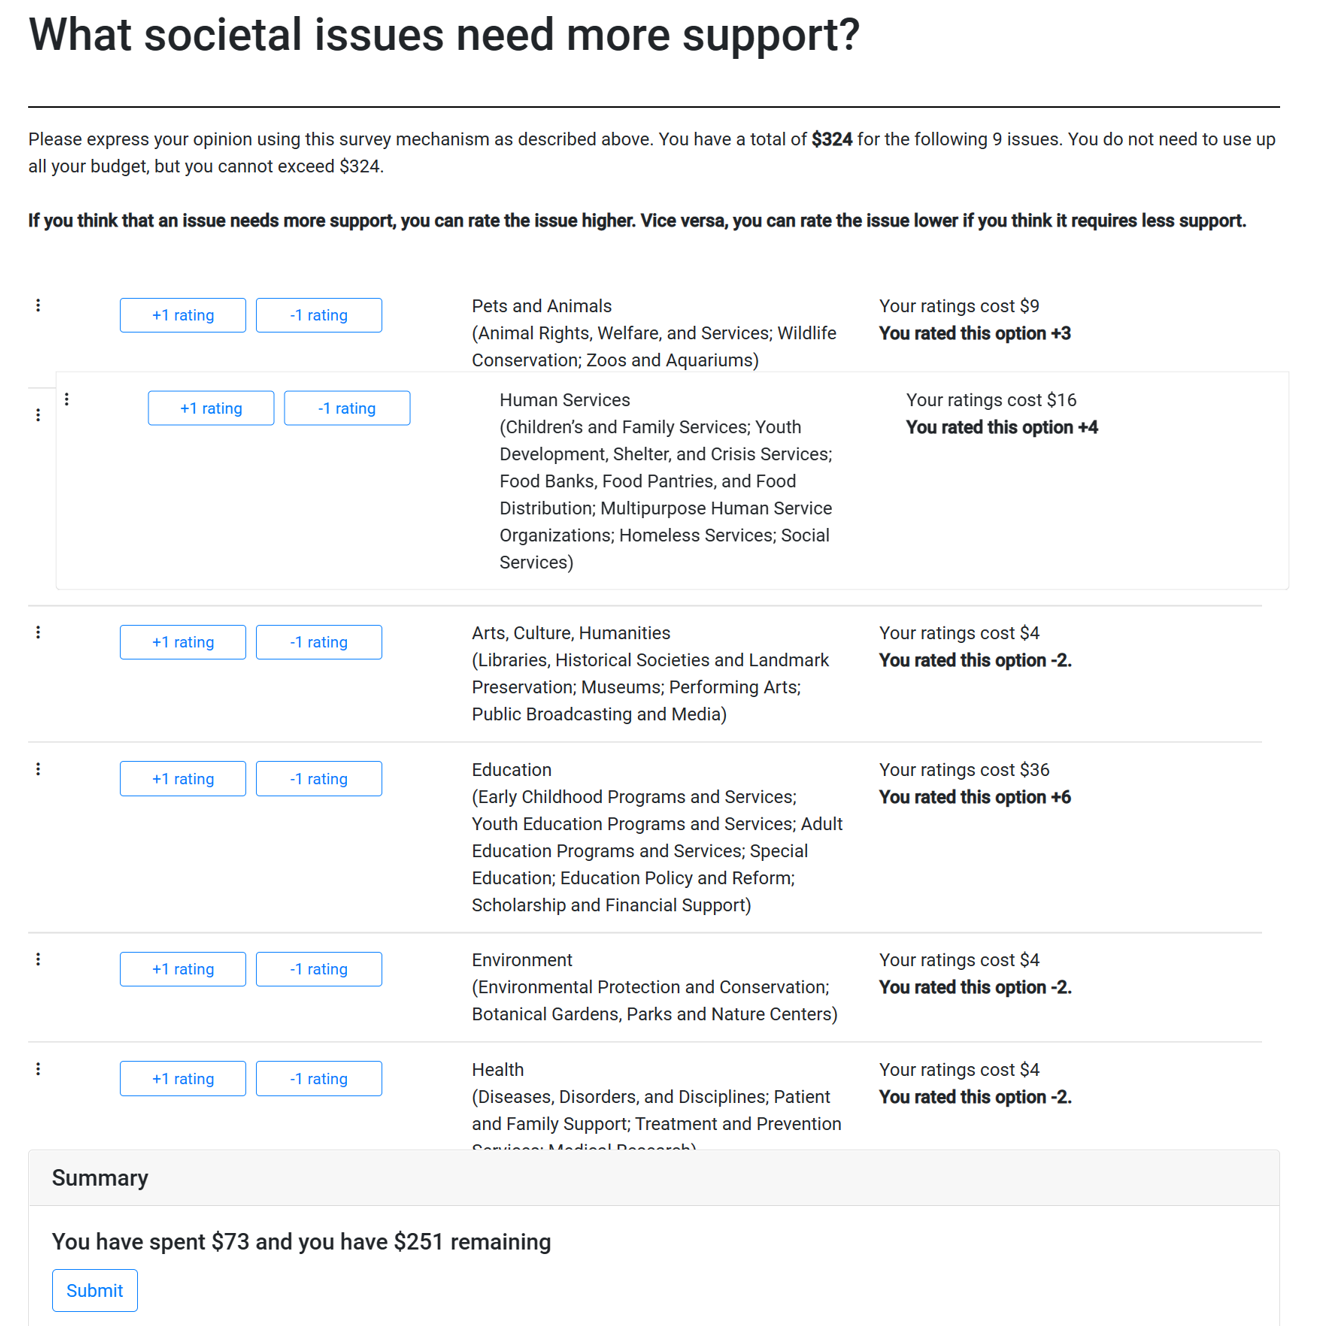
\includegraphics[width=0.43\textwidth, trim={7 7 7 8}, clip]{content/image/prototypes/2_ranking.png}
    \caption{A Ranking-Vote Prototype: This prototype tests whether ranking options prior to voting helps establish an individual's relative preferences. Each option is draggable, allowing users to position it within the full list of options. Votes can be adjusted using the buttons on the left side of the interface, while the vote count and costs are displayed on the right. A summary box remains fixed at the bottom of the screen for easy reference.}
    \Description{A web interface showing a survey titled "What societal issues need more support?" The interface presents several societal issues in a list format, each with buttons labeled "+1 rating" and "-1 rating" to adjust the ratings. For example, the issue "Pets and Animals" shows a rating cost of \$9 with a +3 rating, and "Human Services" shows a rating cost of \$16 with a +4 rating. The remaining issues include Arts, Culture, Humanities, Education, Environment, and Health, each with their respective ratings and costs. At the bottom of the page is a summary box displaying the total spent (\$73) and the remaining balance (\$251). A "Submit" button is positioned below the summary.}
    \label{fig:qv_rank}
    \vspace{-3ex}
\end{figure}

\begin{figure*}[p]
    \centering
    \begin{subfigure}[b]{0.47\textwidth}
        \centering
        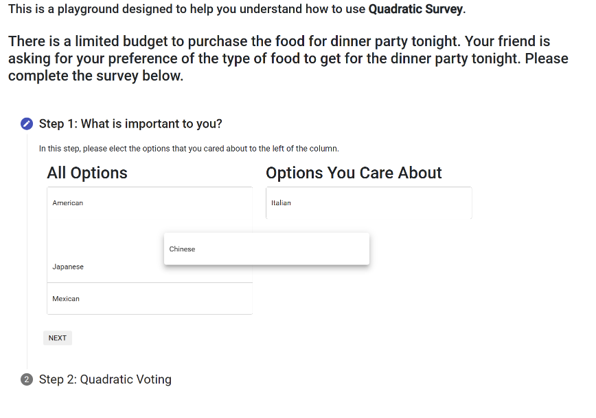
\includegraphics[width=0.95\textwidth]{content/image/prototypes/3.1_selecting.png}
        \caption{Options are dragged and dropped to the 'Option You Care About' box.}
        \Description{A web interface showing the first step of a quadratic voting prototype. The screen is titled "What is important to you?" On the left, under "All Options," a list of food types is displayed, including American, Japanese, and Mexican. One option, "Chinese," is being dragged to the right column labeled "Options You Care About," which already includes "Italian." A "Next" button appears at the bottom of the interface.}

        \label{fig:qv_select_selection}
    \end{subfigure}
    \hfill
    \begin{subfigure}[b]{0.47\textwidth}
        \centering
        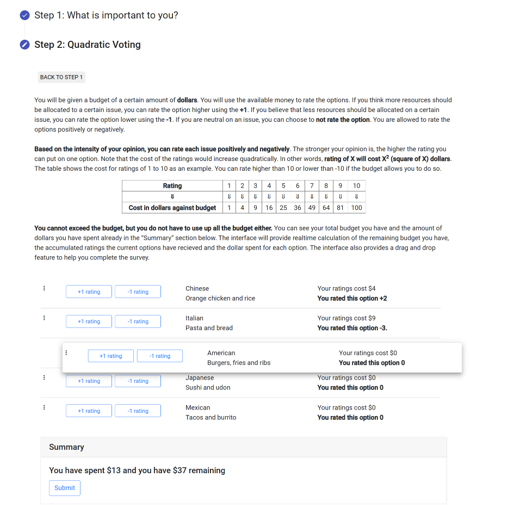
\includegraphics[width=0.9\textwidth]{content/image/prototypes/3.2_selecting_2.png}
        \caption{The previous step collapses showing all voting options.}
        \Description{The second step of a quadratic voting prototype showing a list of food options for voting. The voting interface displays food items such as Chinese, Pasta and bread, and American. Next to each item are "+1 rating" and "-1 rating" buttons for adjusting votes. Each option also shows the cost of votes, and a summary box at the bottom displays the amount spent (\$13) and the remaining balance (\$37).}

        \label{fig:qv_select_vote}
    \end{subfigure}
    \caption{A Select-then-Vote Prototype: The goal of this prototype is to nudge participants to focus on a subset of options to vote, rather than ranking all of them. This prototype introduces a two-step voting process. As shown in Fig.~\ref{fig:qv_select_selection}, the first step involves selecting options for further consideration. Important options are placed at the top of the list for voting shown in Fig.~\ref{fig:qv_select_vote}, but options can be placed anywhere on the list if desired. The rest of the controls follows the previous prototype.}
    \Description{A two-step quadratic voting prototype interface. In the first step (Subfigure 1), users drag and drop food options from a list on the left, such as American and Mexican, to the "Options You Care About" box on the right. In the second step (Subfigure 2), users vote on their selected options by adjusting the ratings using "+1 rating" and "-1 rating" buttons. A summary at the bottom shows the total amount spent and remaining balance.}

    \label{fig:qv_select}
\end{figure*}

\begin{figure*}[p]
    \centering
    \begin{subfigure}[b]{0.45\textwidth}
        \centering
        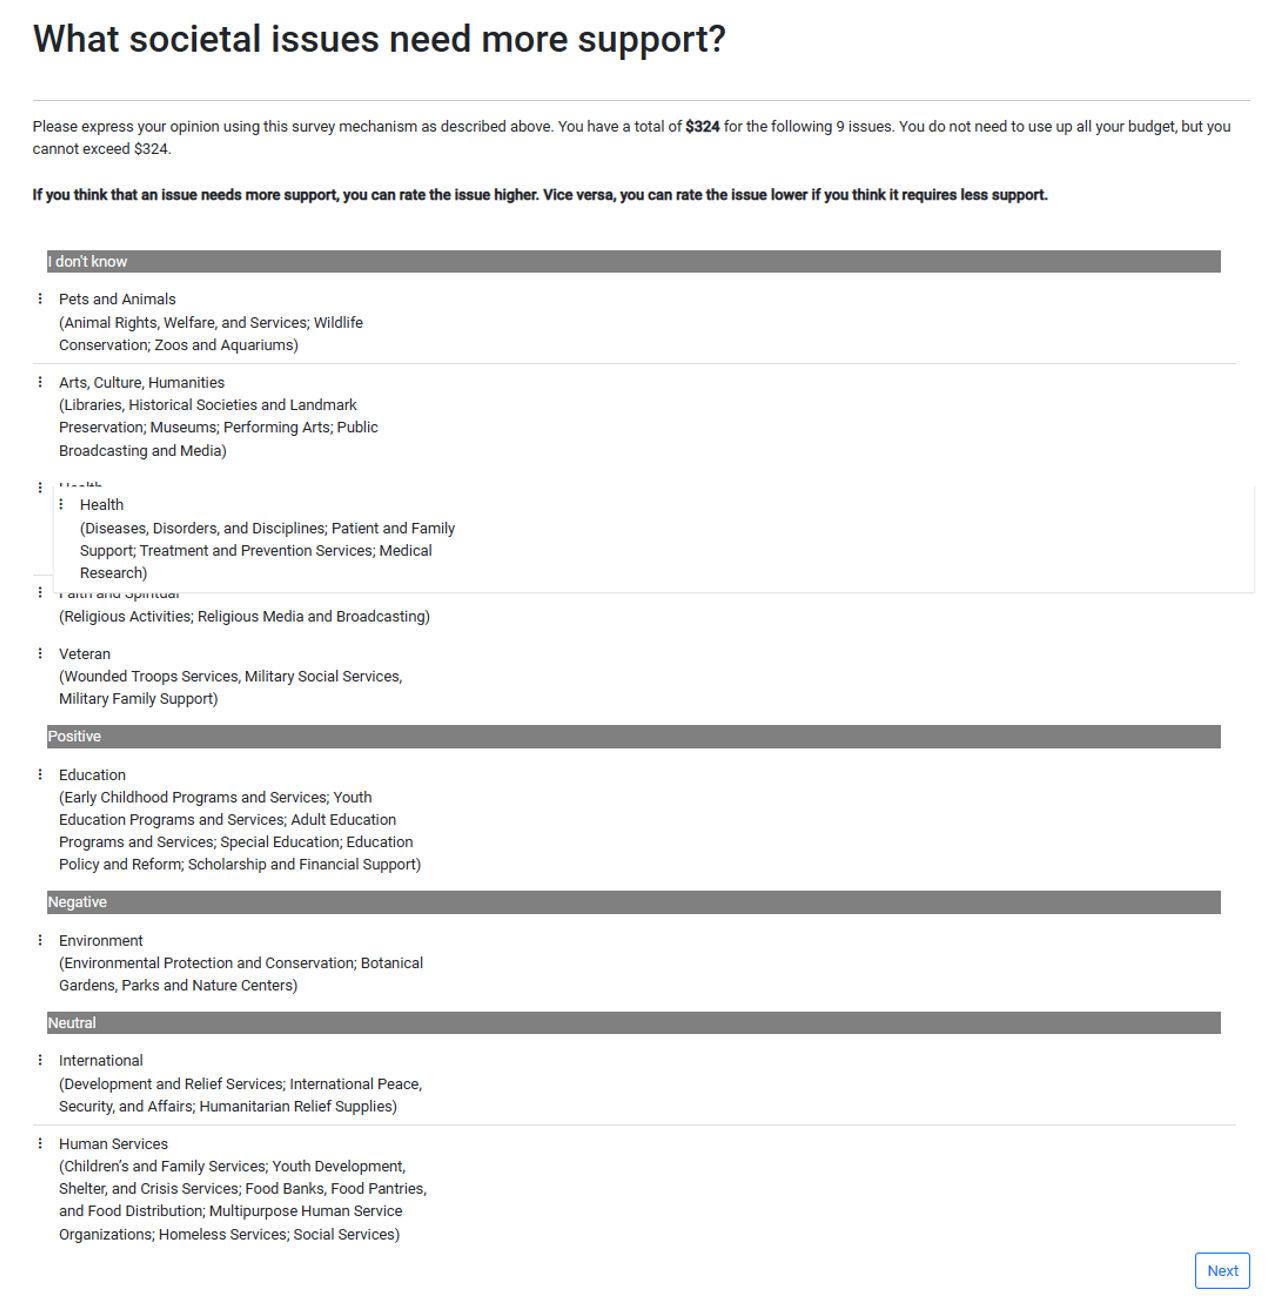
\includegraphics[width=\textwidth]{content/image/prototypes/4.1_grouping.png}
        \caption{The Organization Interface: Options are shown initially in the first bin labeled as `I don't know.' Survey respondents can then drag and drop these options into the latter bins: Lean Positive, Lean Neutral, or Lean Negative. Only the details of each option are shown on this interface.}
        \Description{A web interface displaying a survey titled "What societal issues need more support?" Initially, all options are placed in the first bin labeled "I don't know." The listed options include Pets and Animals, Arts, Culture, Humanities, Health, Veterans, and others. Each option is accompanied by a brief description. Below the "I don't know" bin are three other bins: "Positive," "Negative," and "Neutral." Survey respondents can drag and drop options into these bins based on their preferences. A "Next" button is located at the bottom right corner of the interface.}
        \label{fig:qv_org_p1}
    \end{subfigure}
    \hfill
    \begin{subfigure}[b]{0.45\textwidth}
        \centering
        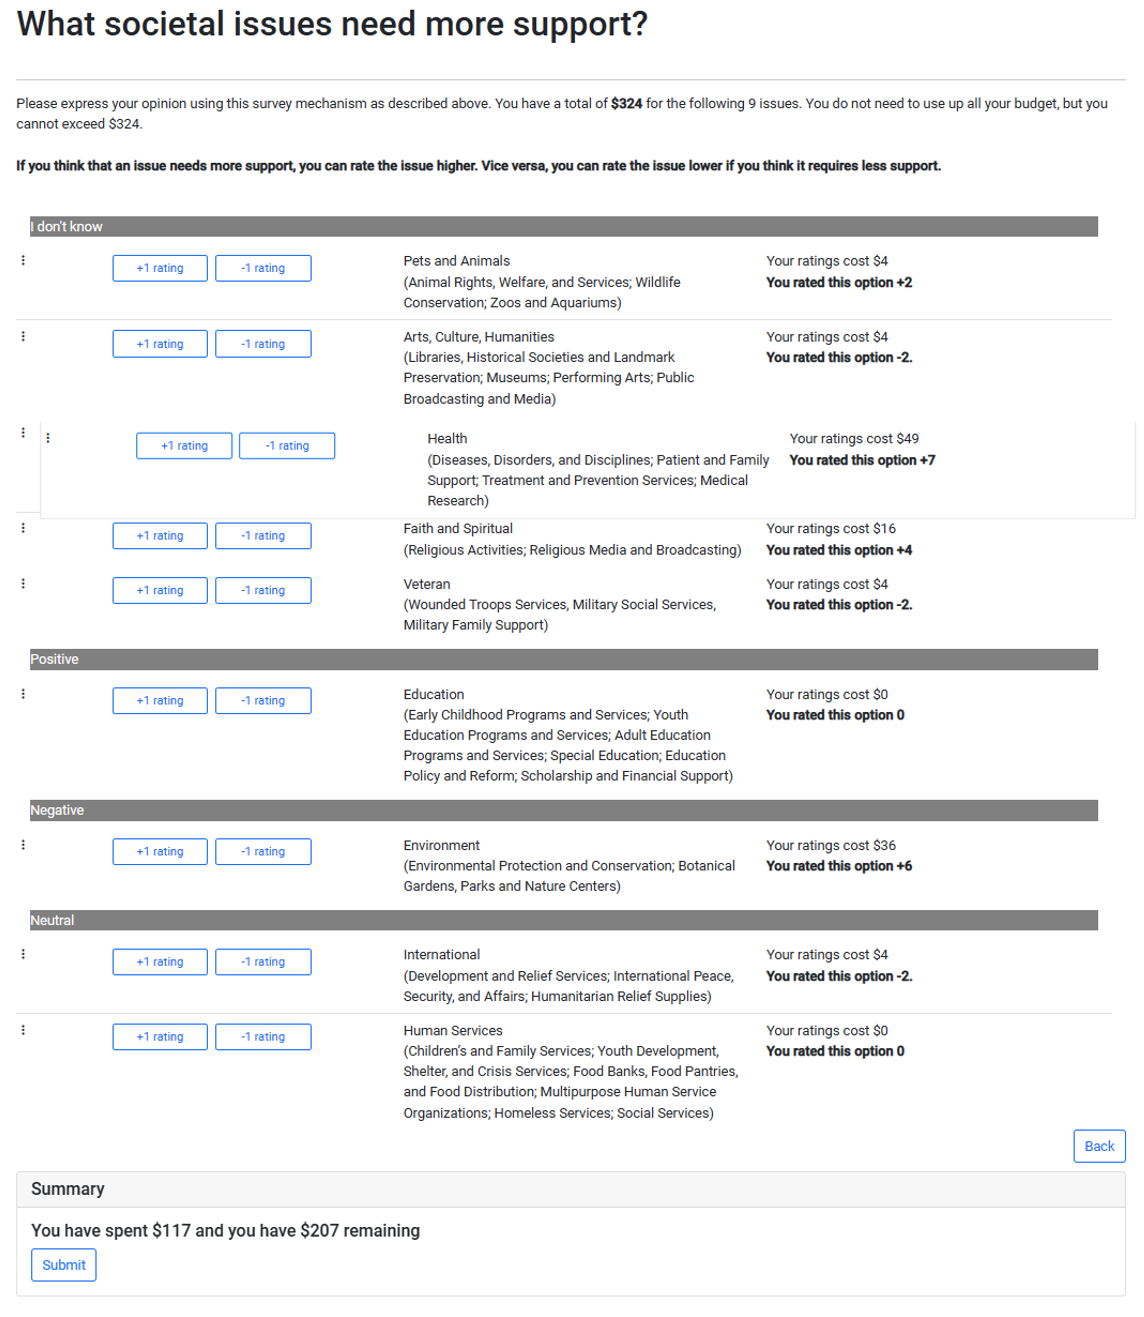
\includegraphics[width=\textwidth]{content/image/prototypes/4.2_grouping_vote.png}
        \caption{The Voting Interface: Voting controls appear on the left side of each option, showing the current votes and associated costs on the right. A budget summary sticks to the bottom of the screen.}
        \Description{A web interface displaying a survey titled "What societal issues need more support?" Each option in the list has voting controls, with "+1 rating" and "-1 rating" buttons appearing on the left side of each issue. The issues are grouped into categories such as "I don't know," "Positive," "Negative," and "Neutral." To the right of each issue, the cost of the rating is shown along with the number of votes cast. For example, "Pets and Animals" has a rating cost of \$4 with a +2 rating, while "Health" has a rating cost of \$49 with a +7 rating. At the bottom of the page, a summary box shows the total amount spent (\$117) and the remaining balance (\$207), with a "Submit" button below it.}

        \label{fig:qv_org_p2}
    \end{subfigure}
    \caption{Organize-then-Vote Prototype: The goal of this prototype is to encourage participants to derive finer grain categories among options before voting. Survey respondents first organize their thoughts into categories and then vote on the options.}
    \Description{The figure shows an Organize-then-Vote prototype with two main steps. In the first step, the left figure, users organize options by dragging and dropping them into different categories: "I don't know," "Positive," "Neutral," or "Negative." In the second step, the right figure, users vote on these organized options using "+1 rating" and "-1 rating" buttons, with voting costs and current ratings displayed. A summary section shows the total spent and remaining budget.}
    \label{fig:qv_org}
\end{figure*}

\subsection{Prototype 2: Select-then-Vote}
Based on feedback from Prototype 1, instead of \textit{allowing} individuals to rank options, Prototype 2 implemented a two-phase process that \textit{intentionally} asks respondents to select options to express opinions before voting. 

As shown in Figure~\ref{fig:qv_select}, survey respondents selected their preferred options (Figure~\ref{fig:qv_select_selection}), and the interface positioned these options at the top of the list for voting (Figure~\ref{fig:qv_select_vote}). We identified several issues during the prototype 2 pretest: many respondents marked most options as 'options they care about,' which undermined the design's purpose. Additionally, the lack of clear distinction between selected and unselected options confused respondents about the necessity of Step 1. Thus, we need a clearer distinction and connection between the two phases to effectively construct relative preferences.

\subsection{Prototype 3: Organize-then-Vote}
Figure~\ref{fig:qv_org} shows the final prototype, which builds on our previous takeaway by introducing finer-grained groupings and establishing a clearer connection between option organization and voting position. Specifically, we provided three categories: Lean Positive, Lean Negative, and Lean Neutral. Initially, respondents see all options listed under a section labeled 'I don't know,' which displays only the option descriptions and not the vote controls. They are then asked to move these options into one of the three categories. On the subsequent page, voting controls and additional information appear for each option, reinforcing the connection between option grouping, position, and voting controls.

Feedback indicated that survey respondents are comfortable with the two-phase organize-then-vote design, demonstrating it as a central strategy for our interface development. However, we identified several areas for enhancement: First, the dragging and dropping mechanism in the organization phase is cumbersome and may inadvertently suggest a ranking process, contrary to our intentions. Second, placing unorganized options at the top of the voting list is counterintuitive. Third, the voting controls are disconnected from the option summaries, dividing attention between the left and right sides of the screen. These insights guided refinements in the final two-phase interface, adhering to the organize-then-vote framework.
 % Done
\section{Voting Interface Breakdown}\label{apdx:relatedVoting}
In this section, we outline additional literature that informed this study. There are two sets of literature that we surveyed: Survey response format and voting interfaces.

\subsection{Survey response format}
Research in the marketing and research communities focusing on survey and questionnaire design, usability, and interactions examines the influence of presentation styles and `response format.'~\citet{weijtersExtremityHorizontalVertical2021} demonstrated that horizontal distances between options are more influential than vertical distances, with the latter recommended for reduced bias. Slider bars, which operate on a drag-and-drop principle, show lower mean scores and higher nonresponse rates compared to buttons, indicating they are more prone to bias and difficult to use. In contrast, visual analog scales that operate on a point-and-click principle perform better~\cite{toepoelSlidersVisualAnalogue2018}. These studies show how even small design changes can have a large impact on usability, highlighting the importance of designing interfaces that prioritize human-centered interaction rather than focusing solely on functionality.

\subsection{Voting Interfaces}
Compared to digital survey interfaces, voting interfaces are a specialized type of survey interface can significantly influence democratic processes~\cite{engstrom2020politics, chisnellDemocracyDesignProblem2016, civicdesignDesigningUsableBallots2015} and often have consequential impacts. Researchers believe that ill-designed voting interfaces We categorize these related works into three main categories detailed below:

\paragraph{Designs that shifted voter decisions: } For example, states without straight-party ticket voting~(where voters can select all candidates from one party through a single choice) exhibited higher rates of split-ticket voting~\cite{engstrom2020politics}. Another example from the Australian ballot showing incumbency advantages is where candidates are listed by the office they are running for, with no party labels or boxes.

\paragraph{Designs that influenced errors: } Butterfly ballots, an atypical design, may have influenced the outcome of the 2000 U.S. Presidential Election~\cite{wandButterflyDidIt2001}. It increased voter errors because voters could not correctly identify the punch hole on the ballot. Splitting contestants across columns increases the chance for voters to overvote~\cite{quesenberyOpinionGoodDesign2020}. On the other hand, \citet{everettElectronicVotingMachines2008} showed the use of incorporating physical voting behaviors, like lever voting, into graphical user interfaces increased satisfaction while maintaining efficiency and effectiveness.

\paragraph{Designs that incorporated technologies: } Other projects like the Caltech-MIT Voting Technology Project addresses accessibility challenges, resulting in innovations like EZ Ballot~\cite{leeUniversalDesignBallot2016}, Anywhere Ballot~\cite{summers2014making}, and Prime III~\cite{dawkinsPrimeIIIInnovative2009}. In addition,~\citet{gilbertAnomalyDetectionElectronic2013} investigated optimal touchpoints on voting interfaces, and~\citet{conradElectronicVotingEliminates2009} examined zoomable voting interfaces.

Response format literature and voting interfaces informed how interfaces significantly influence respondent behavior, decision accuracy, and cognitive load. These burdens are especially problematic for complex systems like QS, where high cognitive demands may deter researchers and users alike. Developing effective, human-centered interfaces for QS could enhance usability, reduce cognitive overload, and increase adoption in both research and practical applications.
 % Done
% \newpage

% % Experimental Setup Appendix
% \section{Experimental Setup}
\section{List of Options}
\label{sec:charityList}
We provide the full list of options presented on the survey.

\begin{itemize}[leftmargin=*]
    \item \textbf{Animal Rights, Welfare, and Services:} Protect animals from cruelty, exploitation and other abuses, provide veterinary services and train guide dogs.
    \item \textbf{Wildlife Conservation:} Protect wildlife habitats, including fish, wildlife, and bird refuges and sanctuaries.
    \item \textbf{Zoos and Aquariums:} Support and invest in zoos, aquariums and zoological societies in communities throughout the country.
    \item \textbf{Libraries, Historical Societies and Landmark Preservation:} Support and invest public and specialized libraries, historical societies, historical preservation programs, and historical estates.
    \item \textbf{Museums:} Support and invest in maintaining collections and provide training to practitioners in traditional arts, science, technology, and natural history.
    \item \textbf{Performing Arts:} Support symphonies, orchestras, and other musical groups; ballets and operas; theater groups; arts festivals; and performance halls and cultural centers.
    \item \textbf{Public Broadcasting and Media:} Support public television and radio stations and networks, as well as providing other independent media and communications services to the public.
    \item \textbf{Community Foundations:} Promote giving by managing long-term donor-advised charitable funds for individual givers and distributing those funds to community-based charities over time.
    \item \textbf{Housing and Neighborhood Development:} Lead and finance development projects that invest in and improve communities by providing utility assistance, small business support programs, and other revitalization projects.
    \item \textbf{Jewish Federations:} Focus on a specific geographic region and primarily support Jewish-oriented programs, organizations and activities through grantmaking efforts
    \item \textbf{United Ways:} Identify and resolve community issues through partnerships with schools, government agencies, businesses, and others, with a focus on education, income and health.
    \item \textbf{Adult Education Programs and Services:} Provide opportunities for adults to expand their knowledge in a particular field or discipline, learn English as a second language, or complete their high school education.
    \item \textbf{Early Childhood Programs and Services:} Provide foundation-level learning and literacy for children prior to entering the formal school setting.
    \item \textbf{Education Policy and Reform:} Promote and provide research, policy, and reform of the management of educational institutions, educational systems, and education policy.
    \item \textbf{Scholarship and Financial Support:} Support and enable students to obtain the financial assistance they require to meet their educational and living expenses while in school.
    \item \textbf{Special Education:} Provide services, including placement, programming, instruction, and support for gifted children and youth or those with disabilities requiring modified curricula, teaching methods, or materials.
    \item \textbf{Youth Education Programs and Services:} Provide programming, classroom instruction, and support for school-aged students in various disciplines such as art education, STEM, outward bound learning experiences, and other programs that enhance formal education.
    \item \textbf{Botanical Gardens, Parks, and Nature Centers:} Promote preservation and appreciation of the environment, as well as leading anti-litter, tree planting and other environmental beautification campaigns.
    \item \textbf{Environmental Protection and Conservation:} Develop strategies to combat pollution, promote conservation and sustainable management of land, water, and energy resources, protect land, and improve the efficiency of energy and waste material usage.
    \item \textbf{Diseases, Disorders, and Disciplines:} Seek cures for diseases and disorders or promote specific medical disciplines by providing direct services, advocating for public support and understanding, and supporting targeted medical research.
    \item \textbf{Medical Research:} Devote and invest in efforts on researching causes and cures of disease and developing new treatments.
    \item \textbf{Patient and Family Support:} Support programs and services for family members and patients that are diagnosed with a serious illness, including wish granting programs, camping programs, housing or travel assistance.
    \item \textbf{Treatment and Prevention Services:} Provide direct medical services and educate the public on ways to prevent diseases and reduce health risks.
    \item \textbf{Advocacy and Education:} Support social justice through legal advocacy, social action, and supporting laws and measures that promote reform and protect civil rights, including election reform and tolerance among diverse groups.
    \item \textbf{Development and Relief Services:} Provide medical care and other human services as well as economic, educational, and agricultural development services to people around the world.
    \item \textbf{Humanitarian Relief Supplies:} Specialize in collecting donated medical, food, agriculture, and other supplies and distributing them overseas to those in need.
    \item \textbf{International Peace, Security, and Affairs:} Promote peace and security, cultural and student exchange programs, improve relations between particular countries, provide foreign policy research and advocacy, and United Nations-related organizations.
    \item \textbf{Religious Activities:} Support and promote various faiths.
    \item \textbf{Religious Media and Broadcasting:} Support organizations of all faiths that produce and distribute religious programming, literature, and other communications.
    \item \textbf{Non-Medical Science \& Technology Research:} Support research and services in a variety of scientific disciplines, advancing knowledge and understanding of areas such as energy efficiency, environmental and trade policies, and agricultural sustainability.
    \item \textbf{Social and Public Policy Research:} Support economic and social issues impacting our country today, educate the public, and influence policy regarding healthcare, employment rights, taxation, and other civic ventures.
\end{itemize}


% \begin{table}[h!]
% \centering
% \caption{Full List of Survey Options}
% \label{tab:optionsList}
% \begin{tabular}{p{3.4cm} p{12cm}}
% \toprule
% \textbf{Category} & \textbf{Description} \\
% \midrule
% Animal Rights, Welfare, and Services & Protect animals from cruelty, exploitation, and other abuses, provide veterinary services, and train guide dogs. \\
% Wildlife Conservation & Protect wildlife habitats, including fish, wildlife, and bird refuges and sanctuaries. \\
% Zoos and Aquariums & Support and invest in zoos, aquariums, and zoological societies in communities throughout the country. \\
% Libraries, Historical Societies, and Landmark Preservation & Support public and specialized libraries, historical societies, preservation programs, and historical estates. \\
% Museums & Support and invest in maintaining collections and providing training to practitioners in traditional arts, science, technology, and natural history. \\
% Performing Arts & Support symphonies, orchestras, ballets, operas, theater groups, arts festivals, and cultural centers. \\
% Public Broadcasting and Media & Support public television and radio stations and networks, as well as independent media and communications services. \\
% Community Foundations & Promote giving by managing donor-advised charitable funds and distributing them to community-based charities over time. \\
% Housing and Neighborhood Development & Lead and finance projects to improve communities by providing utility assistance, small business support, and revitalization projects. \\
% Jewish Federations & Support Jewish-oriented programs, organizations, and activities through grantmaking efforts. \\
% United Ways & Identify and resolve community issues through partnerships with schools, government agencies, businesses, and others. \\
% Adult Education Programs and Services & Provide opportunities for adults to expand their knowledge, learn English as a second language, or complete their high school education. \\
% Early Childhood Programs and Services & Provide foundation-level learning and literacy for children before formal schooling. \\
% Education Policy and Reform & Promote research, policy, and reform of educational institutions and systems. \\
% Scholarship and Financial Support & Support students to obtain financial assistance for educational and living expenses. \\
% Special Education & Provide services for gifted children and youth or those with disabilities requiring modified curricula or teaching methods. \\
% Youth Education Programs and Services & Provide programming for school-aged students in disciplines such as art, STEM, and outward-bound learning. \\
% Botanical Gardens, Parks, and Nature Centers & Promote preservation of the environment and lead environmental beautification campaigns. \\
% Environmental Protection and Conservation & Develop strategies to combat pollution, promote conservation, and manage resources sustainably. \\
% Diseases, Disorders, and Disciplines & Seek cures for diseases and disorders and promote specific medical disciplines. \\
% Medical Research & Research causes and cures of diseases and develop new treatments. \\
% Patient and Family Support & Support programs for family members and patients diagnosed with serious illnesses. \\
% Treatment and Prevention Services & Provide medical services and educate the public on disease prevention and health risks. \\
% Advocacy and Education & Support social justice through legal advocacy, social action, and reform measures. \\
% Development and Relief Services & Provide medical care, human services, and economic, educational, and agricultural development services. \\
% Humanitarian Relief Supplies & Distribute donated medical, food, agricultural, and other supplies to those in need. \\
% International Peace, Security, and Affairs & Promote peace, security, cultural exchanges, and improve international relations. \\
% Religious Activities & Support and promote various faiths. \\
% Religious Media and Broadcasting & Support organizations producing religious programming and literature. \\
% Non-Medical Science \& Technology Research & Support research in scientific disciplines, advancing knowledge in areas like energy efficiency and sustainability. \\
% Social and Public Policy Research & Support research on economic and social issues impacting healthcare, employment, taxation, and civic policies. \\
% \bottomrule
% \end{tabular}
% \end{table}
     % Done
\section{Demographic Breakdown}
\label{sec:apdx:demo}
\Cref{tab:age_gender_distribution} provides a detailed demographic breakdown per group.
\begin{table*}[h!]
\centering
\caption{Participant Age and Gender Distribution by Experimental Condition}
\label{tab:age_gender_distribution}
\begin{tabular}{lcccccccccc}
\hline
\textbf{Condition} & \textbf{Mean Age} & \textbf{SD} & \textbf{Range} & \textbf{25th} & \textbf{Median} & \textbf{75th} & \textbf{Male} & \textbf{Female} & \textbf{Non-binary} \\
\hline
Short Text      & 31.6  & 13.7 & 18--67 & 23.8 & 29.5 & 32.8 & 4 & 6 & 0 \\
Short Two-Phase   & 32.1  & 14.0 & 18--52 & 20.3 & 27.0 & 44.5 & 4 & 6 & 0 \\
Long Text       & 36.0  & 14.8 & 21--61 & 24.0 & 33.0 & 42.8 & 2 & 7 & 1 \\
Long Two-Phase    & 38.8  & 19.6 & 19--71 & 25.0 & 28.5 & 53.0 & 2 & 8 & 0 \\
\hline
\end{tabular}
\Description{ A table summarizing participant demographics and descriptive statistics for four conditions: Short Text, Short 2-Phase, Long Text, and Long 2-Phase.}
\end{table*}
 % Done


% % Results Appendix
% \section{Results}
\begin{figure*}[t!]
    \centering
    \begin{minipage}[t]{0.32\textwidth}
        \centering
        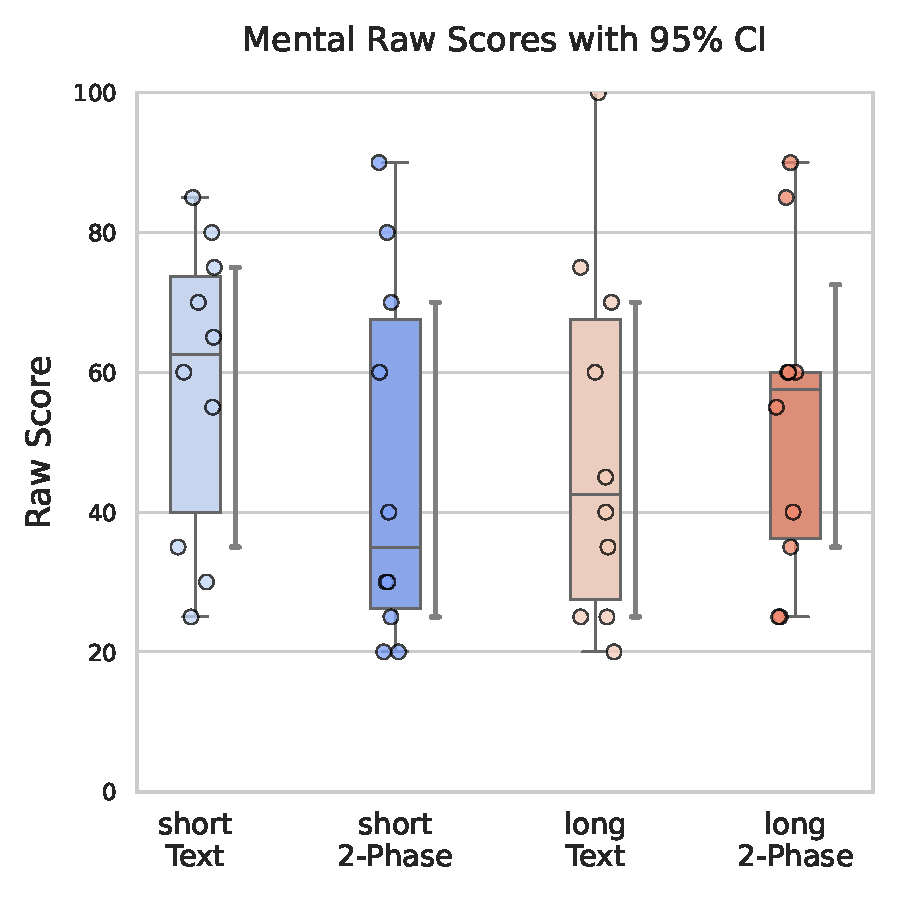
\includegraphics[width=\textwidth, trim=0 13 0 13, clip]{content/image/cog/Mental_scores.pdf}
        \caption{Mental Demand Raw Score: Across all four experiment groups, participants' reported mental demand is spread across a wide range with many participants experiencing high mental demand.}
        \Description{Box plot showing mental raw scores with 95\% confidence intervals across four interface versions: Short Text, Short 2-Phase, Long Text, and Long 2-Phase. The y-axis represents raw scores from 0 to 100. Each box plot includes individual data points. The Short Text and Short 2-Phase versions display wider score distributions, with medians around 60 and 40. The Long Text and Long 2-Phase versions have similar distributions but with slightly lower medians, 40 and 60, respectively. The plot shows a considerable spread in scores, with overlapping confidence intervals, indicating variability in mental demand across all groups.}
        \label{fig:mental_cog_score}
    \end{minipage}%
    \hfill
    \begin{minipage}[t]{0.32\textwidth}
        \centering
        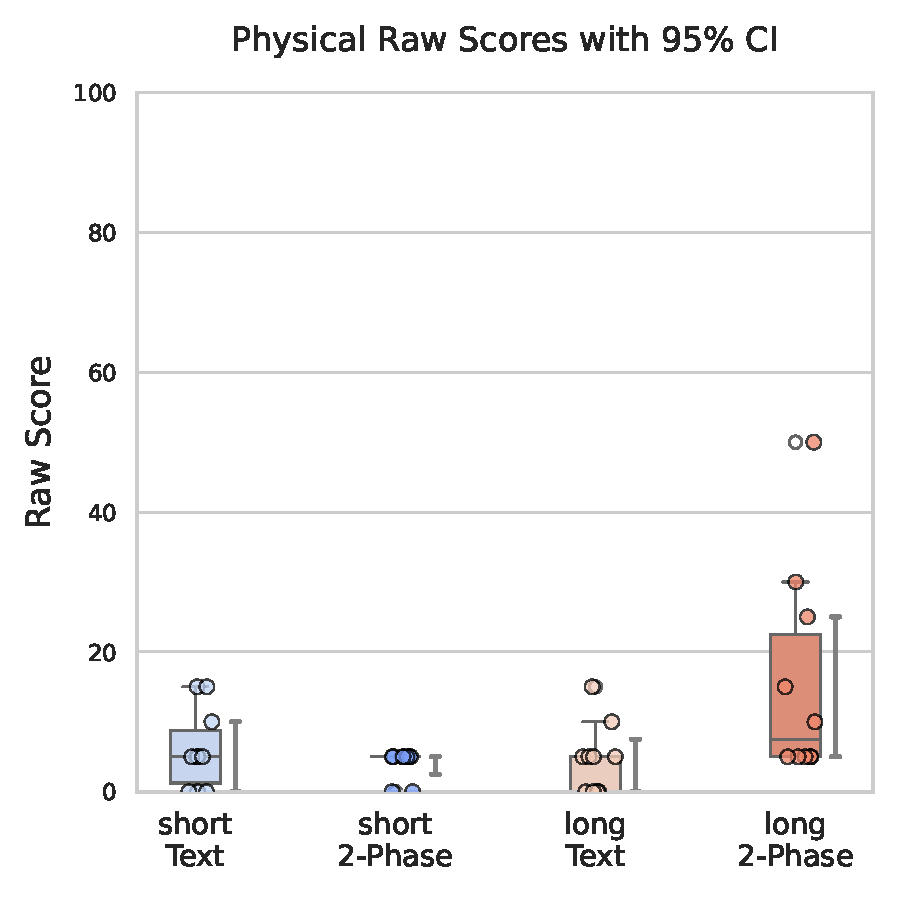
\includegraphics[width=\textwidth, trim=0 13 0 13, clip]{content/image/cog/Physical_scores.pdf}
        \caption{Physical Demand Raw Score: Participants other than the long two-phase interface reported minimal physical demand. The long two-phase interface had the highest physical demand, likely due to increased mouse clicks and extended time spent looking at the vertical screen.}
        \Description{A box plot showing the distribution of physical raw scores across four interface versions: Short Text, Short 2-Phase, Long Text, and Long 2-Phase. The y-axis represents the raw score ranging from 0 to 100. The box plots include individual data points, a central line for the median, and whiskers indicating the 95\% confidence interval. The Short Text, Short 2-Phase, and Long Text interfaces show minimal physical demand, with scores clustered below 20. The Long 2-Phase interface exhibits higher physical demand, with a few scores scattered up to around 60.}
        \label{apdxfig:physical_cog_score}
    \end{minipage}%
    \hfill
    \begin{minipage}[t]{0.32\textwidth}
        \centering
        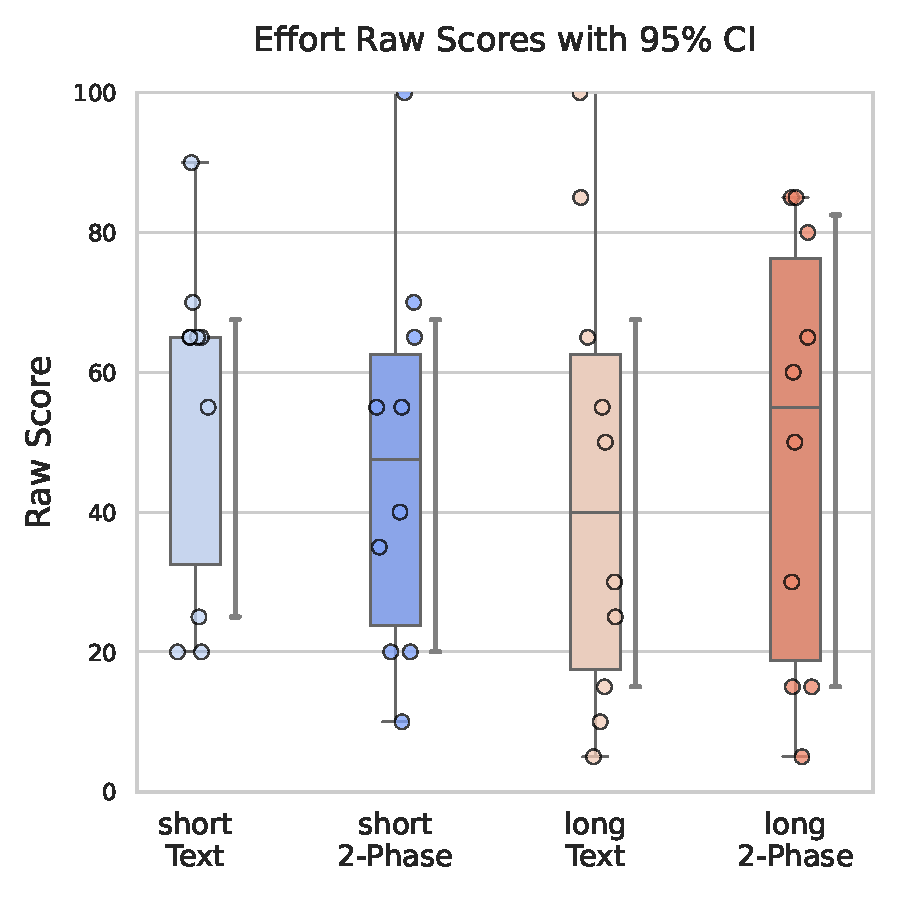
\includegraphics[width=\textwidth, trim=0 13 0 13, clip]{content/image/cog/Effort_scores.pdf}
        \caption{Effort Raw Score: Effort scores show indifference across groups. All groups had high variance of responses indicating some participants requires high amount of effort when completing QS regardless of length and interface}
        \Description{A box plot showing the distribution of effort raw scores across four interface versions: Short Text, Short 2-Phase, Long Text, and Long 2-Phase. The y-axis represents the raw score ranging from 0 to 100. Each box plot includes individual data points, a central line indicating the median, and whiskers representing the 95\% confidence interval. The Long 2-Phase interface shows the widest range of effort scores, while the other interfaces display more compact distributions. Data points are scattered within and outside the whiskers, reflecting variability in effort scores across the groups.}
        \label{apdxfig:effort_cog_score}
    \end{minipage}
\end{figure*}

\section{Detailed Qualitative Cognitive Load Breakdown}
\label{apdx:cog_qual}

We provide additional details on the six cognitive dimensions. Among all dimensions, we also provide the codes representing different types of demand in a table form. The shaded cells represent the percentage of participants citing each source of mental demand, allowing for comparison within columns. The abbreviations in the columns: ST (Short Text Interface), S2P (Short Two-phase Interface), LT (Long Text Interface), and L2P (Long Two-phase Interface). Short and Long refer to the sum across both interfaces; Text and 2P (Two-phase interface) refer to the sum across both survey lengths. We include Sparklines for comparisons across these experiment groups. Future studies can use these as initial codebooks to conduct interface studies on preference construction.

\begin{table*}[p]
   \caption{This table lists all the causes participants mentioned as contributing to their Mental Demand.}
   \Description{A table presenting mental demand across categories such as Budget Management (track credits, maximize usage), Preference Construction (prioritization, resource allocation), and Demand from Experiment Setup. Sparklines and percentage bars are used to visually represent the data across four interface versions (ST, S2P, LT, L2P) and experiment conditions (Short, Long, Text, Inter). The bars show higher mental demand in areas like Budget Management and Preference Construction, with trends highlighted by sparklines. Additional categories, such as External Factors and Demand due to Interface, are also represented with percentage bars.}
    \label{tbl:mental}
    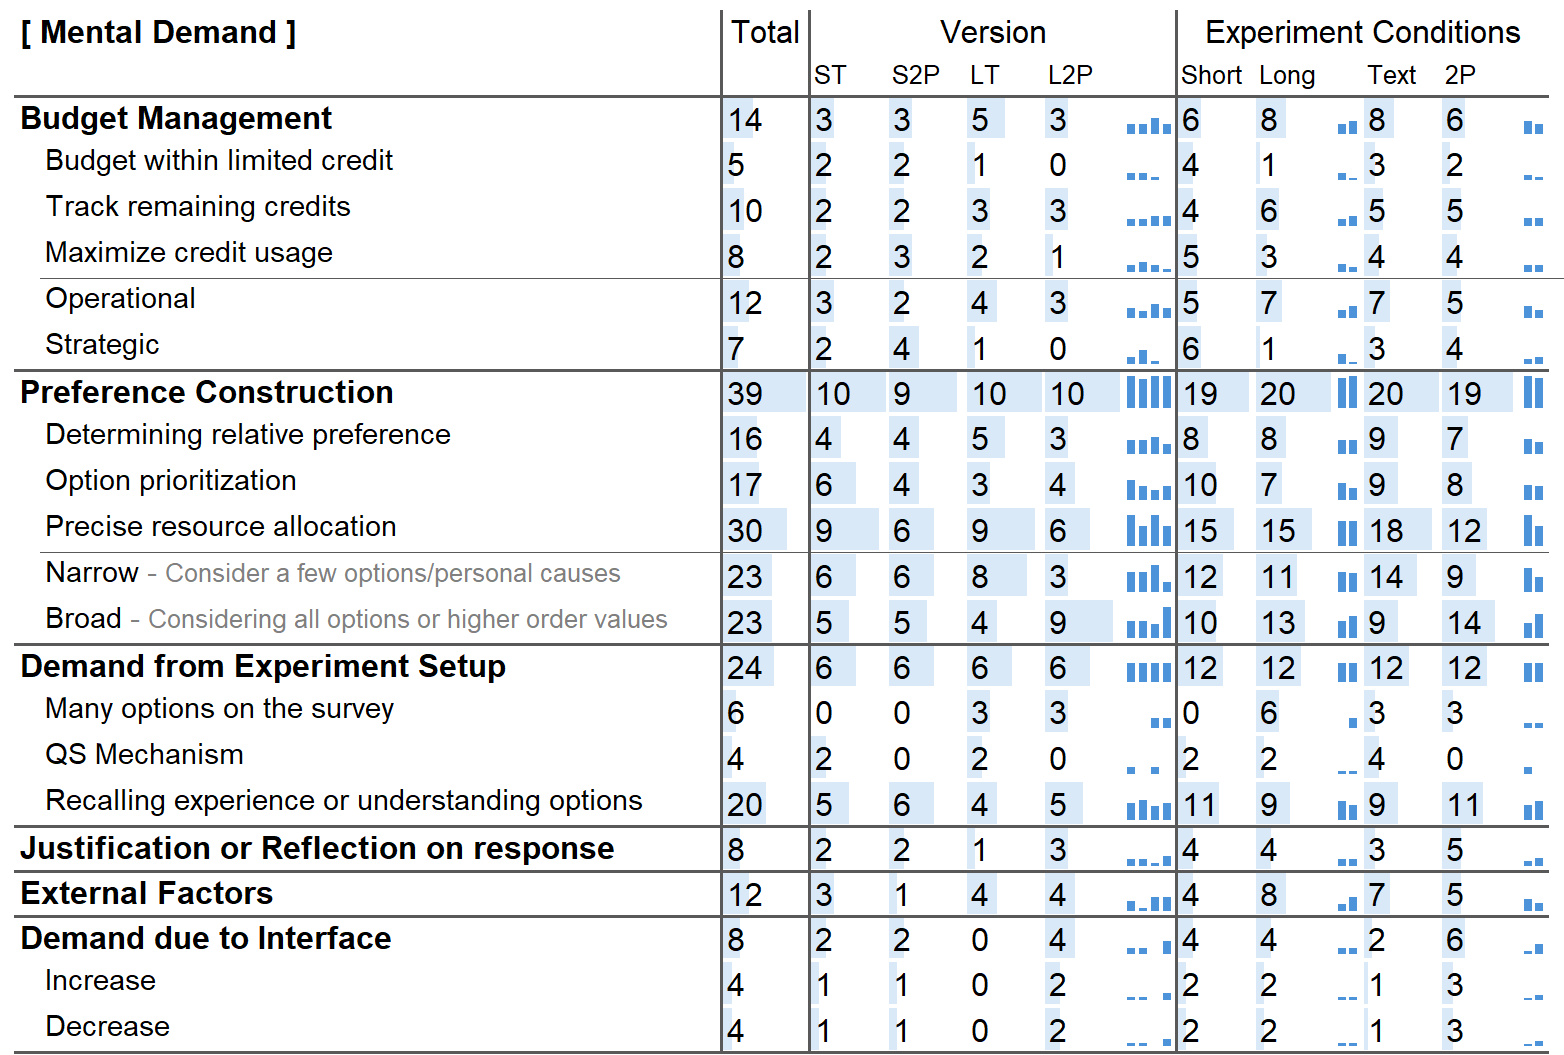
\includegraphics[width=0.85\linewidth]{content/image/cog/mental_table.png}
\end{table*}

\begin{table*}[p]
    \caption{Physical Demand Causes: Most participants expressed little or no physical demand. Results reflected that participants in the long two-phase interface required more actions, hence the higher mention of mouse usage as a source.}
    \Description{A table showing physical challenges experienced by participants, including Reading, Mouse, Vertical Screen, and None/Little physical effort, with sparklines and percentage bars visualizing the data trends. Data is split across four interface versions (ST, S2P, LT, L2P) and experiment conditions (Short, Long, Text, Inter). The Mouse category has the highest counts, with trends clearly visible via sparklines and bars, while Reading and Vertical Screen challenges have lower values. The None/Little row shows participants reporting minimal physical effort with percentage bars illustrating the distribution.}
    \label{apdx:physical_table}
    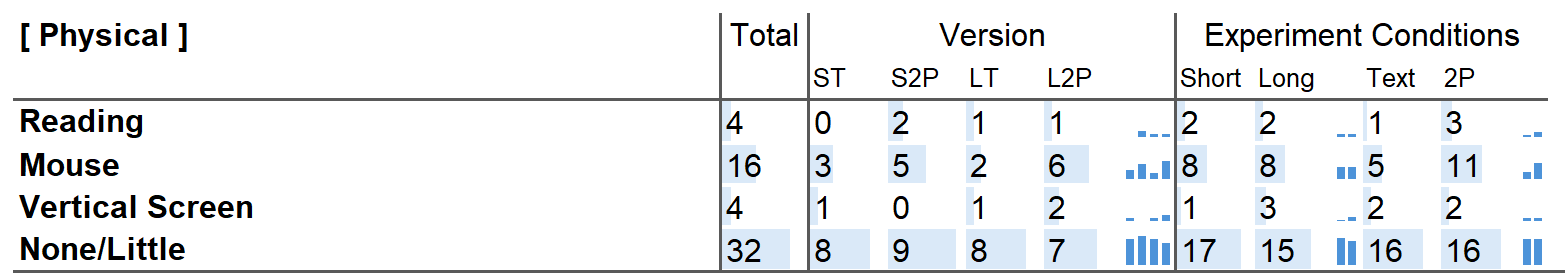
\includegraphics[width=0.85\linewidth]{content/image/cog/physical_table.png}
\end{table*}

\begin{table*}[p]
    \caption{Effort Sources: Participants using the text interface focused more on operational tasks, while those using the two-phase interface focused more on strategic planning.}
    \Description{A table summarizing participant effort as Operational and Strategic (personal and global), with data visualized using sparklines and percentage bars. The table is split into four versions (ST, S2P, LT, L2P) and experiment conditions (Short, Long, Text, Inter), with counts and corresponding bars for each category. The operational effort shows participants managing tasks, while the strategic effort captures balancing personal preferences with societal concerns. Sparklines highlight trends across different conditions. A None/Little/A bit row shows participants exerting minimal effort, visualized with bars.}

    \label{apdx:effort_table}
    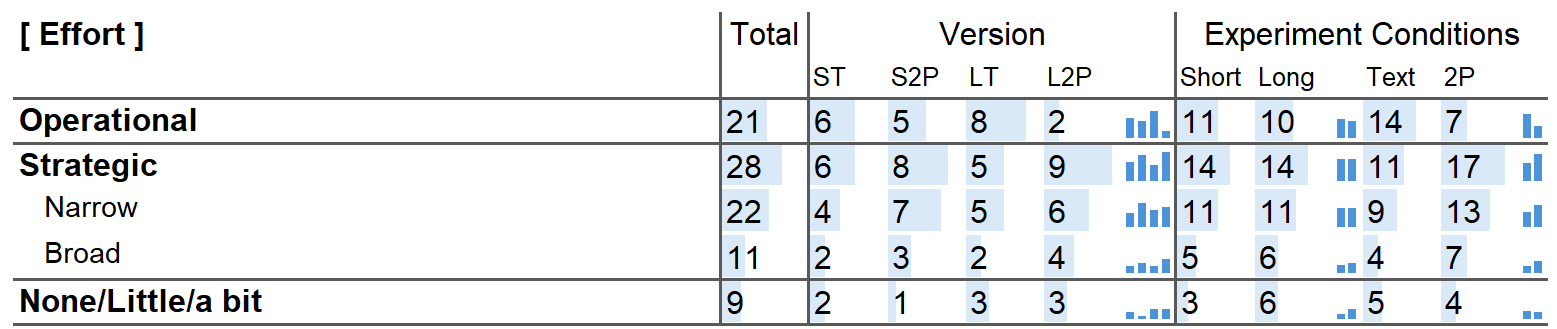
\includegraphics[width=0.85\linewidth]{content/image/cog/effort_table.png}
\end{table*}

\subsection{Sources of Mental Demand}
\label{apdx:mental}
Mental demand refers to the amount of mental and perceptual activity required to complete a task.~\Cref{tbl:mental} lists all qualitative codes and ~\Cref{fig:mental_cog_score} shows the boxplot of participant's subscale response. For thematic groups, we grouped them as source of demand (e.g., tracking remaining credits) and also of scope (e.g., Operational) as separated by the light gray line within each row.

\subsection{Sources of Physical Demand} 
\label{apdx:physical}
Physical demand refers to the physical effort required to complete a task, such as physical exertion or movement. Most participants reported minimal physical demand~($N=32$), reflected in the low NASA-TLX physical demand scores~(Figure~\ref{apdxfig:physical_cog_score}). Notably, $11$ out of $20$ participants who used the two-phase interface mentioned physical demand from using the mouse, reflecting interacting with two interfaces. This is further supported by the raw NASA-TLX physical demand scores~(Figure~\ref{apdxfig:physical_cog_score}), which show a significant visual difference between short and long two-phase interfaces as well as between text and two-phase interfaces in long surveys. Table~\ref{apdx:physical_table} presents all the relevant codes across experiment groups.




% \begin{figure}[t!]
%     \centering
%     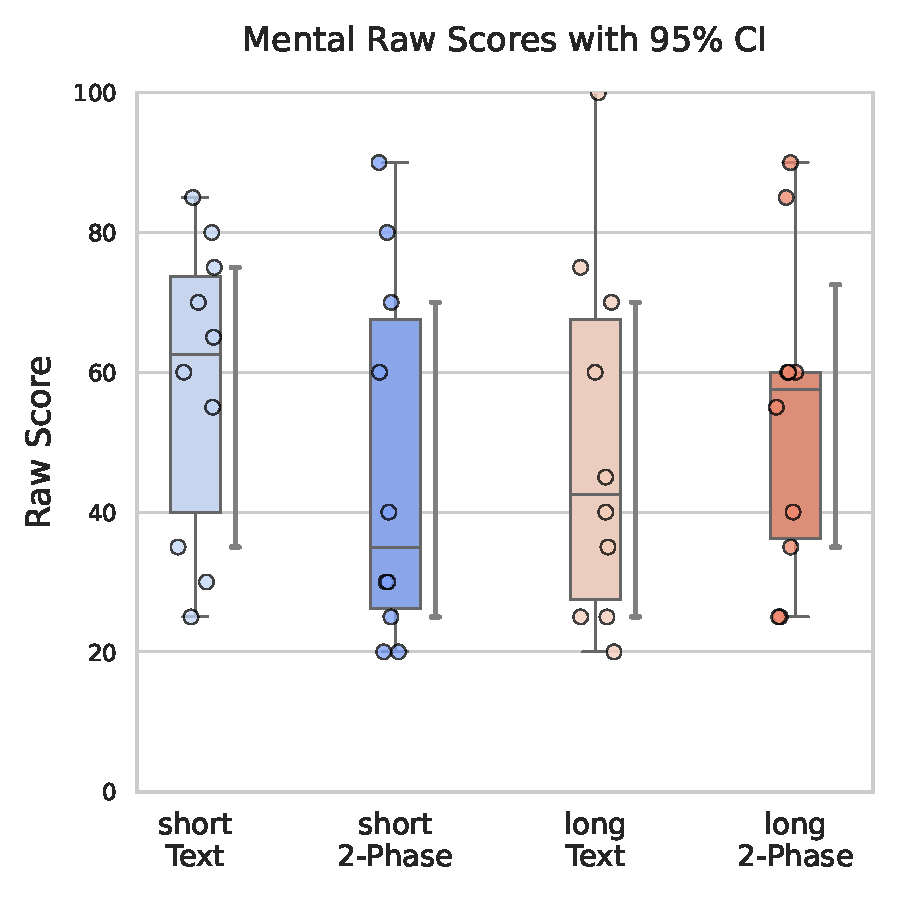
\includegraphics[width=0.38\textwidth, trim=0 13 0 13, clip]{content/image/cog/Mental_scores.pdf}
%     \caption{Mental Demand Raw Score: Across all four experiment groups, participants' reported mental demand is spread across a wide range with many participants experiencing high mental demand.}
%     \Description{Box plot showing mental raw scores with 95\% confidence intervals across four interface versions: Short Text, Short 2-Phase, Long Text, and Long 2-Phase. The y-axis represents raw scores from 0 to 100. Each box plot includes individual data points. The Short Text and Short 2-Phase versions display wider score distributions, with medians around 60 and 40. The Long Text and Long 2-Phase versions have similar distributions but with slightly lower medians, 40 and 60, respectively. The plot shows a considerable spread in scores, with overlapping confidence intervals, indicating variability in mental demand across all groups.}
%     \label{fig:mental_cog_score}
% \end{figure}

% \begin{figure}[h]
%     \centering
%     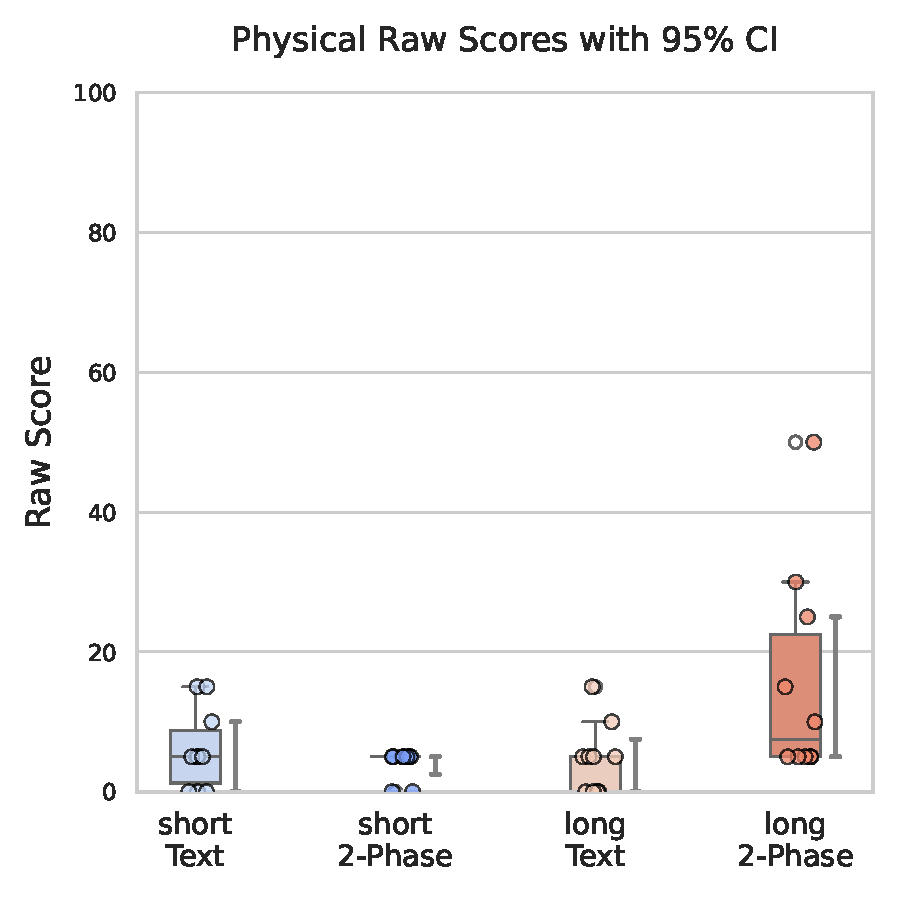
\includegraphics[width=0.38\textwidth, trim=0 13 0 13, clip]{content/image/cog/Physical_scores.pdf}
%     % \captionsetup{width=0.9\linewidth, justification=justified}
%     \caption{Physical Demand Raw Score: Participants other than the long two-phase interface reported minimal physical demand. The long two-phase interface had the highest physical demand, likely due to increased mouse clicks and extended time spent looking at the vertical screen.}
%     \Description{A box plot showing the distribution of physical raw scores across four interface versions: Short Text, Short 2-Phase, Long Text, and Long 2-Phase. The y-axis represents the raw score ranging from 0 to 100. The box plots include individual data points, a central line for the median, and whiskers indicating the 95\% confidence interval. The Short Text, Short 2-Phase, and Long Text interfaces show minimal physical demand, with scores clustered below 20. The Long 2-Phase interface exhibits higher physical demand, with a few scores scattered up to around 60.}
%     \label{apdxfig:physical_cog_score}
% \end{figure}

% \begin{figure}[h]
%     \centering
%     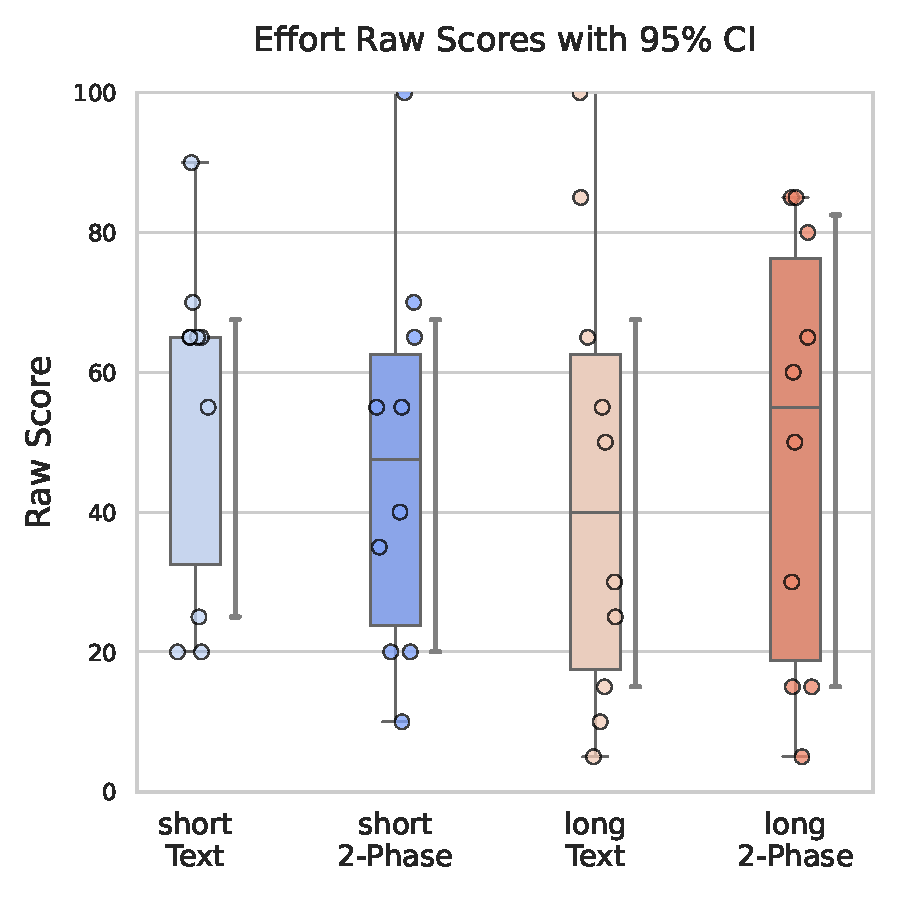
\includegraphics[width=0.38\textwidth, trim=0 13 0 13, clip]{content/image/cog/Effort_scores.pdf}
%     % \captionsetup{width=0.9\linewidth, justification=justified}
%     \caption{Effort Raw Score: Effort scores show indifference across groups.}
%     \Description{A box plot showing the distribution of effort raw scores across four interface versions: Short Text, Short 2-Phase, Long Text, and Long 2-Phase. The y-axis represents the raw score ranging from 0 to 100. Each box plot includes individual data points, a central line indicating the median, and whiskers representing the 95\% confidence interval. The Long 2-Phase interface shows the widest range of effort scores, while the other interfaces display more compact distributions. Data points are scattered within and outside the whiskers, reflecting variability in effort scores across the groups.}
%     \label{apdxfig:effort_cog_score}
% \end{figure}



% ============================================= %

\begin{table*}[p]
    \caption{Performance Causes: Most causes are shared across experiment conditions. We provided qualitative interpretations of their own performance assessments.}
    \Description{A table detailing participant performance across Operational Action (budget control, preference reflection, limited resources), Social Responsibility (decision maker, outcome uncertainty), and Performance Assessment (did their best, feel good, good enough). The table includes sparklines and percentage bars to visualize the distribution of performance data across four interface versions (ST, S2P, LT, L2P) and experiment conditions (Short, Long, Text, Inter). Operational action and social responsibility are visually represented, with sparklines highlighting performance trends.}

    \label{tbl:perf}
    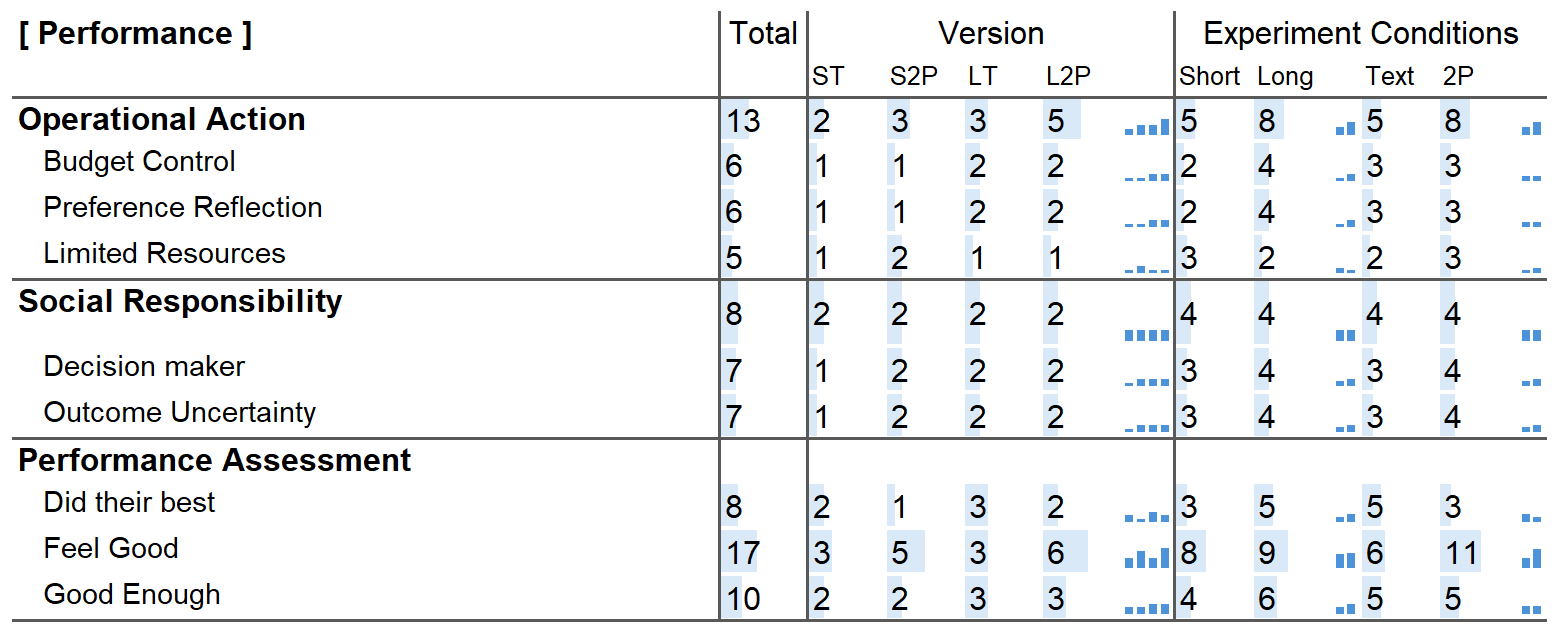
\includegraphics[width=0.85\linewidth]{content/image/cog/perf_table.png}
\end{table*}
\begin{table*}[p]
    \caption{Temporal Demand Sources: Decision-making and Operational Tasks are the main causes. Participants framed their decision-making sources differently.}
    \Description{A table categorizing temporal challenges across Budget Management, Decision Making (affirmative and negative), and Operational (task completion, efficiency). The data includes sparklines and percentage bars to visualize patterns across four versions (ST, S2P, LT, L2P) and experiment conditions (Short, Long, Text, Inter). Affirmative decision-making shows higher values than negative decision-making, with percentage bars indicating the relative distribution. Temporal operational tasks show consistent effort across conditions, as reflected in the sparklines.}

    \label{tbl:temporal}
    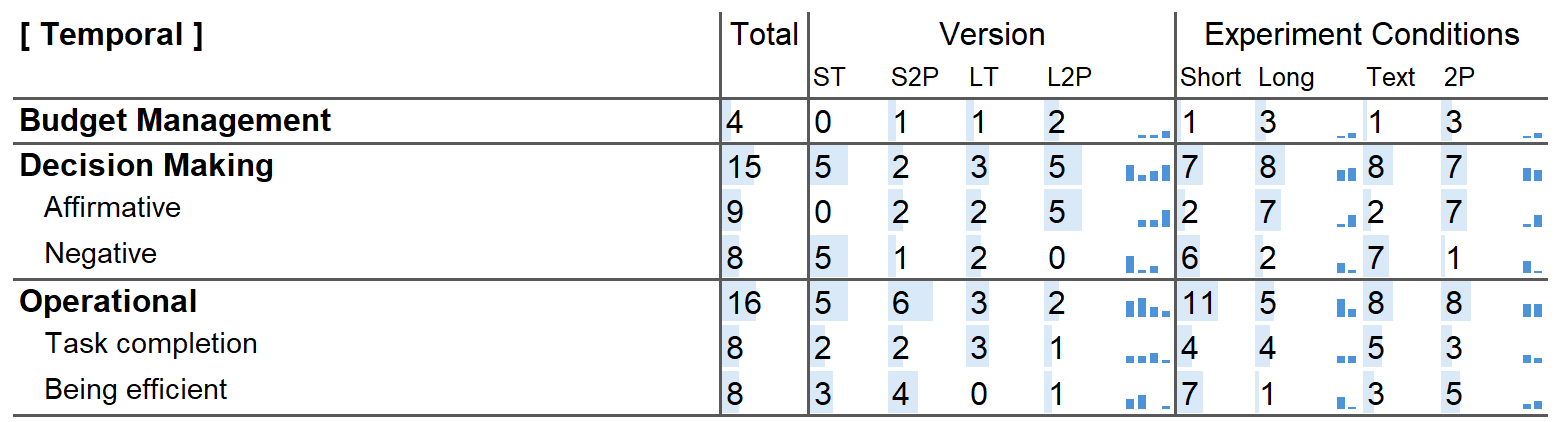
\includegraphics[width=0.85\linewidth]{content/image/cog/temporal_table.png}
\end{table*}


\subsection{Source of Effort}
\label{apdx:effort}
Effort refers to how hard participants felt they worked to achieve the level of performance they did. Since effort includes both mental and physical resource intensity, refer to \Cref{apdx:mental} and \Cref{apdx:physical} for definitions. Raw NASA-TLX effort scores~(Figure~\ref{apdxfig:effort_cog_score}) showed a similar spread across experiment groups, the qualitative analysis showed more distinction that participants using the two-phase interface considered options more comprehensively and felt less effort on completing operational tasks, similar to what we found on mental demands~(Section \ref{apdx:mental}). For this subscale, we grouped codes through the lens of scope. Table~\ref{apdx:effort_table} contains codes. 

$14$ of the $20$ participants using the text interface mentioned operational tasks as a source of effort, compared to $7$ participants using the two-phase interface, with the lowest mention in the long two-phase interface group~($N=2$).

\begin{displayquote}
I wanted to bump up~(an option) maybe to 4 or <option> to 5 and realize I couldn't.~\bracketellipsis that would be effort came in of how do I want to really rearrange this to make it~(the budget spending) maximize?

\noindent \hfill -- S029, short text interface
\end{displayquote}

In contrast, strategic planning was reported as an effort source by $11$ participants in the text interface, compared to $17$ participants in the two-phase interface, with nearly all participants in the long two-phase interface group~($N=9$) expressing effort related to it. In this subscale, we further categorize strategic planning into \textit{narrow} and \textit{broad} scopes as we did for mental demand~(\Cref{apdx:mental}). Participants using the two-phase interface~($N=7$) had nearly mentioned double~($N=4$) times regarding global strategies. For example:

\begin{displayquote}
~\bracketellipsis the effort was how to rank order these~(options) and allocate the resources behind the upvotes so that I can accurately depict what I want~\ldots say, a committee to focus on and allocate actual fungible resources, too. \noindent \hfill -- S019, long two-phase interface
\end{displayquote}




\begin{table*}[p]
    \caption{Frustration Sources: Frustration comes from different levels of strategic operations or operational tasks.}
    \Description{A table with sparklines showing frustration categories: Strategic (higher-level and lower-level) and Operational, across four versions (ST, S2P, LT, L2P) and experiment conditions (Short, Long, Text, Inter). The table includes sparklines and percentage bars alongside the numerical counts to visually represent the data distribution across conditions. Strategic frustration is divided into higher-level and lower-level conflicts between personal preference and broader societal values. Operational frustration includes challenges such as credit management, adhering to the quadratic mechanism, making decisions, and understanding options. A final row captures participants reporting None/Little frustration, also visualized with percentage bars.}

    \label{tbl:fustration}
    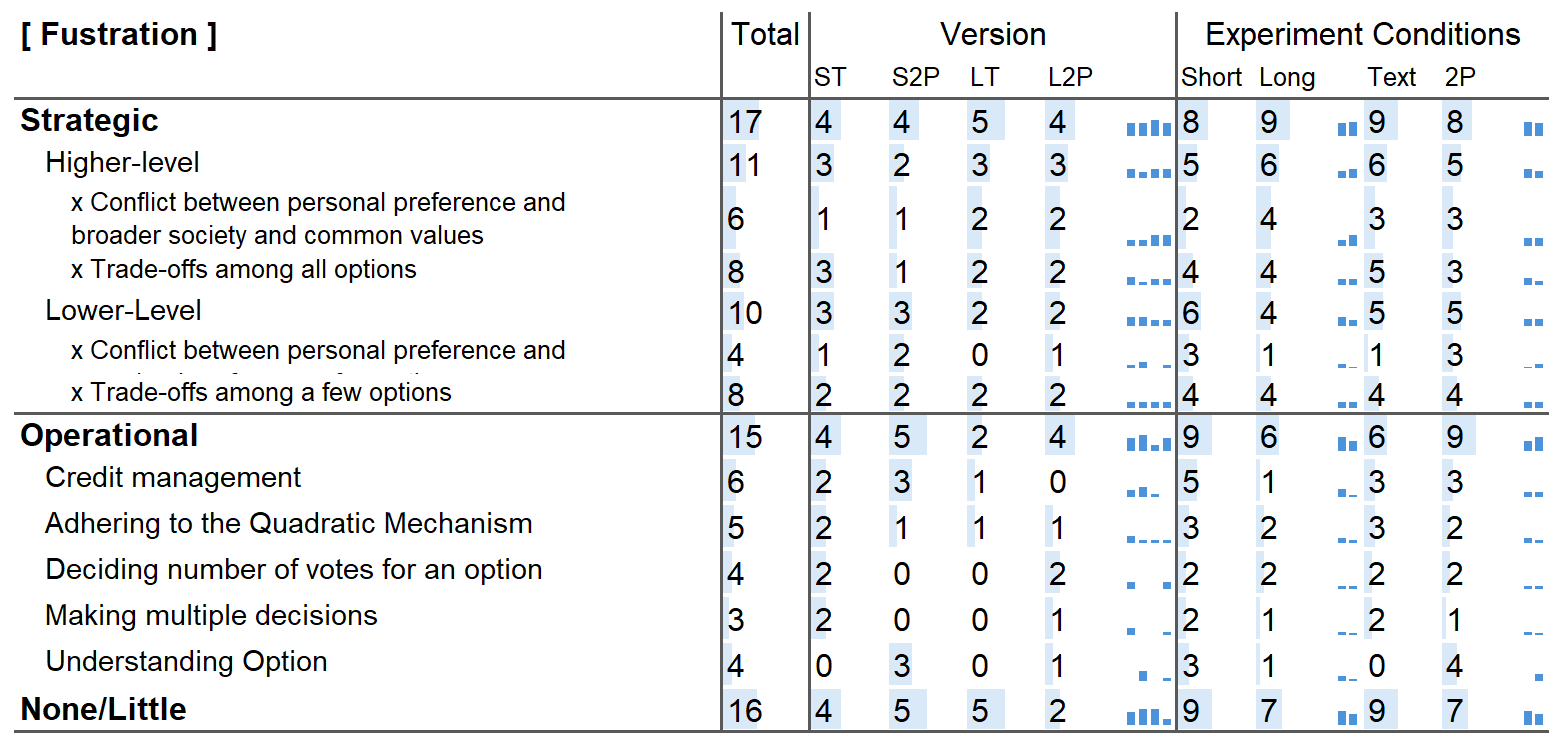
\includegraphics[width=0.85\linewidth]{content/image/cog/fustration_table.png}
\end{table*}

\subsection{Source from Performance}
\label{apdx:performance}

Performance refers to a person's perception of how successfully they have completed a task. Lower values indicate good perceived performance, while higher values suggest poor perceived performance. Raw NASA-TLX scores~(Figure~\ref{fig:performance_cog_score}) show that participants had similar performance scores, although we highlighted nuanced differences in the main text. In addition to the differences mentioned in the main text, an interesting theme that emerged across experimental conditions was that participants' identified that \textit{Social Responsibility} influenced their performance scores.~\Cref{tbl:perf} presents a detailed breakdown of our codes.

\paragraph{Social Responsibility.} This theme refers to concerns about performance when participants reflected on how their final vote counts would be perceived by others~(\smallquote{S041}{I don't want people to think that I just don't care about <ethnicity> people at all}) or how their votes might influence real-world decision-making~(\smallquote{S027}{Some of these things might \ldots have outcomes that I didn't foresee}).

\begin{figure}[h]
    \centering
    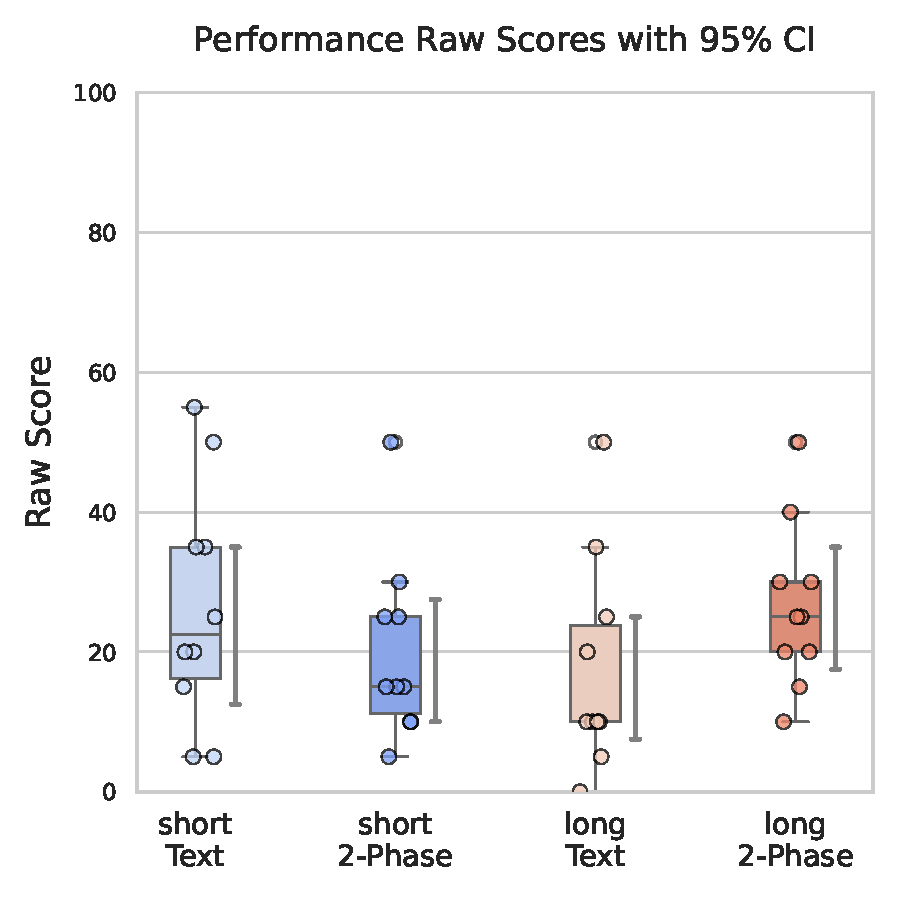
\includegraphics[width=0.38\textwidth, trim=0 13 0 13, clip]{content/image/cog/Performance_scores.pdf}
    \captionsetup{width=0.9\linewidth, justification=justified}
    \caption{Performance Demand Raw Score: Participants showed indifferent performance raw scores across experiment conditions, all trending toward satisfactory.}
    \Description{A box plot displaying the distribution of performance raw scores across four interface versions: Short Text, Short 2-Phase, Long Text, and Long 2-Phase. The y-axis represents raw scores ranging from 0 to 100. Each box plot includes individual data points, a central line for the median, and whiskers representing the 95\% confidence interval. The performance scores appear relatively low across all conditions, with medians hovering between 20 and 40.}
    \label{fig:performance_cog_score}
\end{figure}

\subsection{Temporal Demand}
\label{apdx:temporal}
Table~\ref{tbl:temporal} lists all the temporal demand codes.


\subsection{Frustration}
\label{apdx:frus}
Table~\ref{tbl:fustration} lists all codes related to participants' sources of frustration.


\begin{figure}[h]
    \centering
    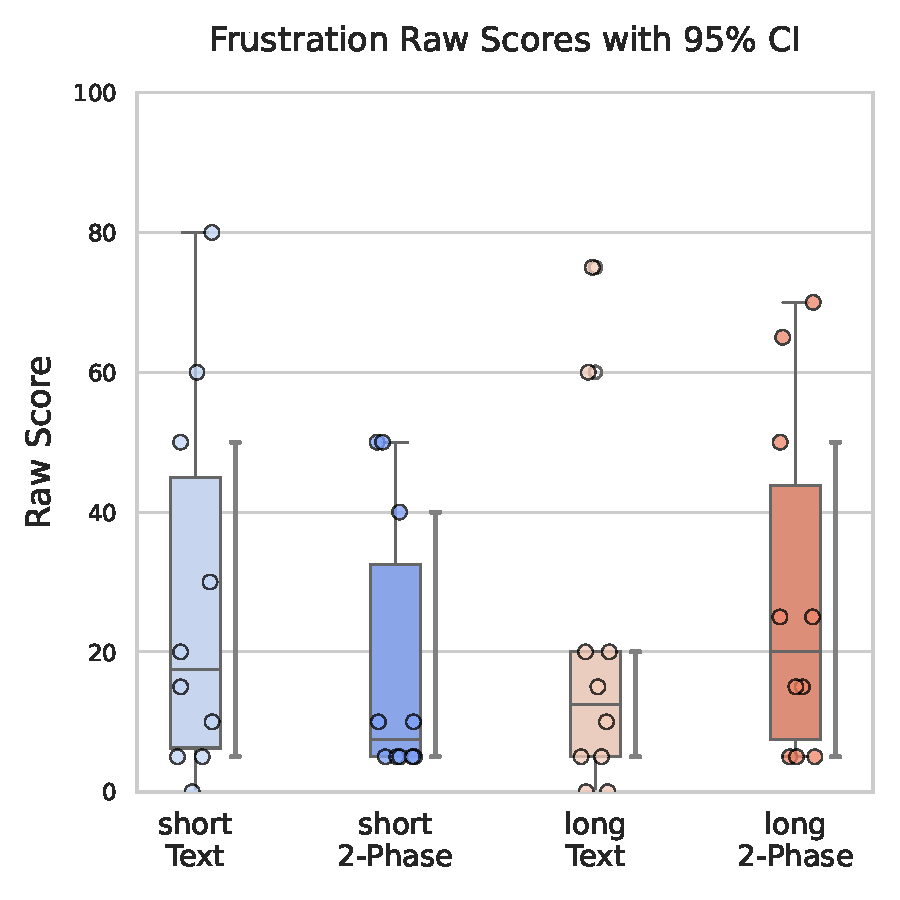
\includegraphics[width=0.38\textwidth, trim=0 13 0 13, clip]{content/image/cog/Frustration_scores.pdf}
    \captionsetup{width=0.9\linewidth, justification=justified}
    \caption{Frustration Raw Score: Participants other than the long text interface highlighted several operational tasks that led to frustration. All groups share causes from strategic planning.}
    \Description{Box plot showing frustration raw scores with 95\% confidence intervals across four interface versions: Short Text, Short 2-Phase, Long Text, and Long 2-Phase. The y-axis represents raw scores from 0 to 100. The Short Text interface has a wide range of scores, with several participants reporting high frustration. The Short 2-Phase interface shows lower median frustration with a narrower distribution. The Long Text interface displays the lowest frustration scores, while the Long 2-Phase interface shows a wide range, with some participants reporting high frustration. Individual data points are included, indicating variability across participants.}
    \label{fig:frustration_cog_score}
\end{figure}
\section{Additional voting behavior data}
\label{apdx:additional_results_behavior}
In this section, we describe additional voting behavior that we observed. The reason why we decided to focus on the percentage of remaining credits comes from prior literature `scarcity frames value'~\cite{Shah2015a}, a driver that makes researchers believe makes quadratic voting more accurate~\cite{chengCanShowWhat2021}. We did not follow~\citet{quarfoot2017quadratic} in counting accumulated votes over time due to varying total times across individuals.

We observed the number of vote adjustments given a remaining vote credit percentage. Figure~\ref{apdxfig:voting_all} showed all the voting actions over the remaining credit for the four experiment conditions. Here we see two distinct patterns between the short survey and the long survey in terms of participant behaviors. In long surveys, participants exhibited more actions both when the budget was abundant and when it began to run out. This pattern was more pronounced with the long two-phase interface. This difference is why we further focused on the long QS group.

\begin{figure*}[p]
    \centering
    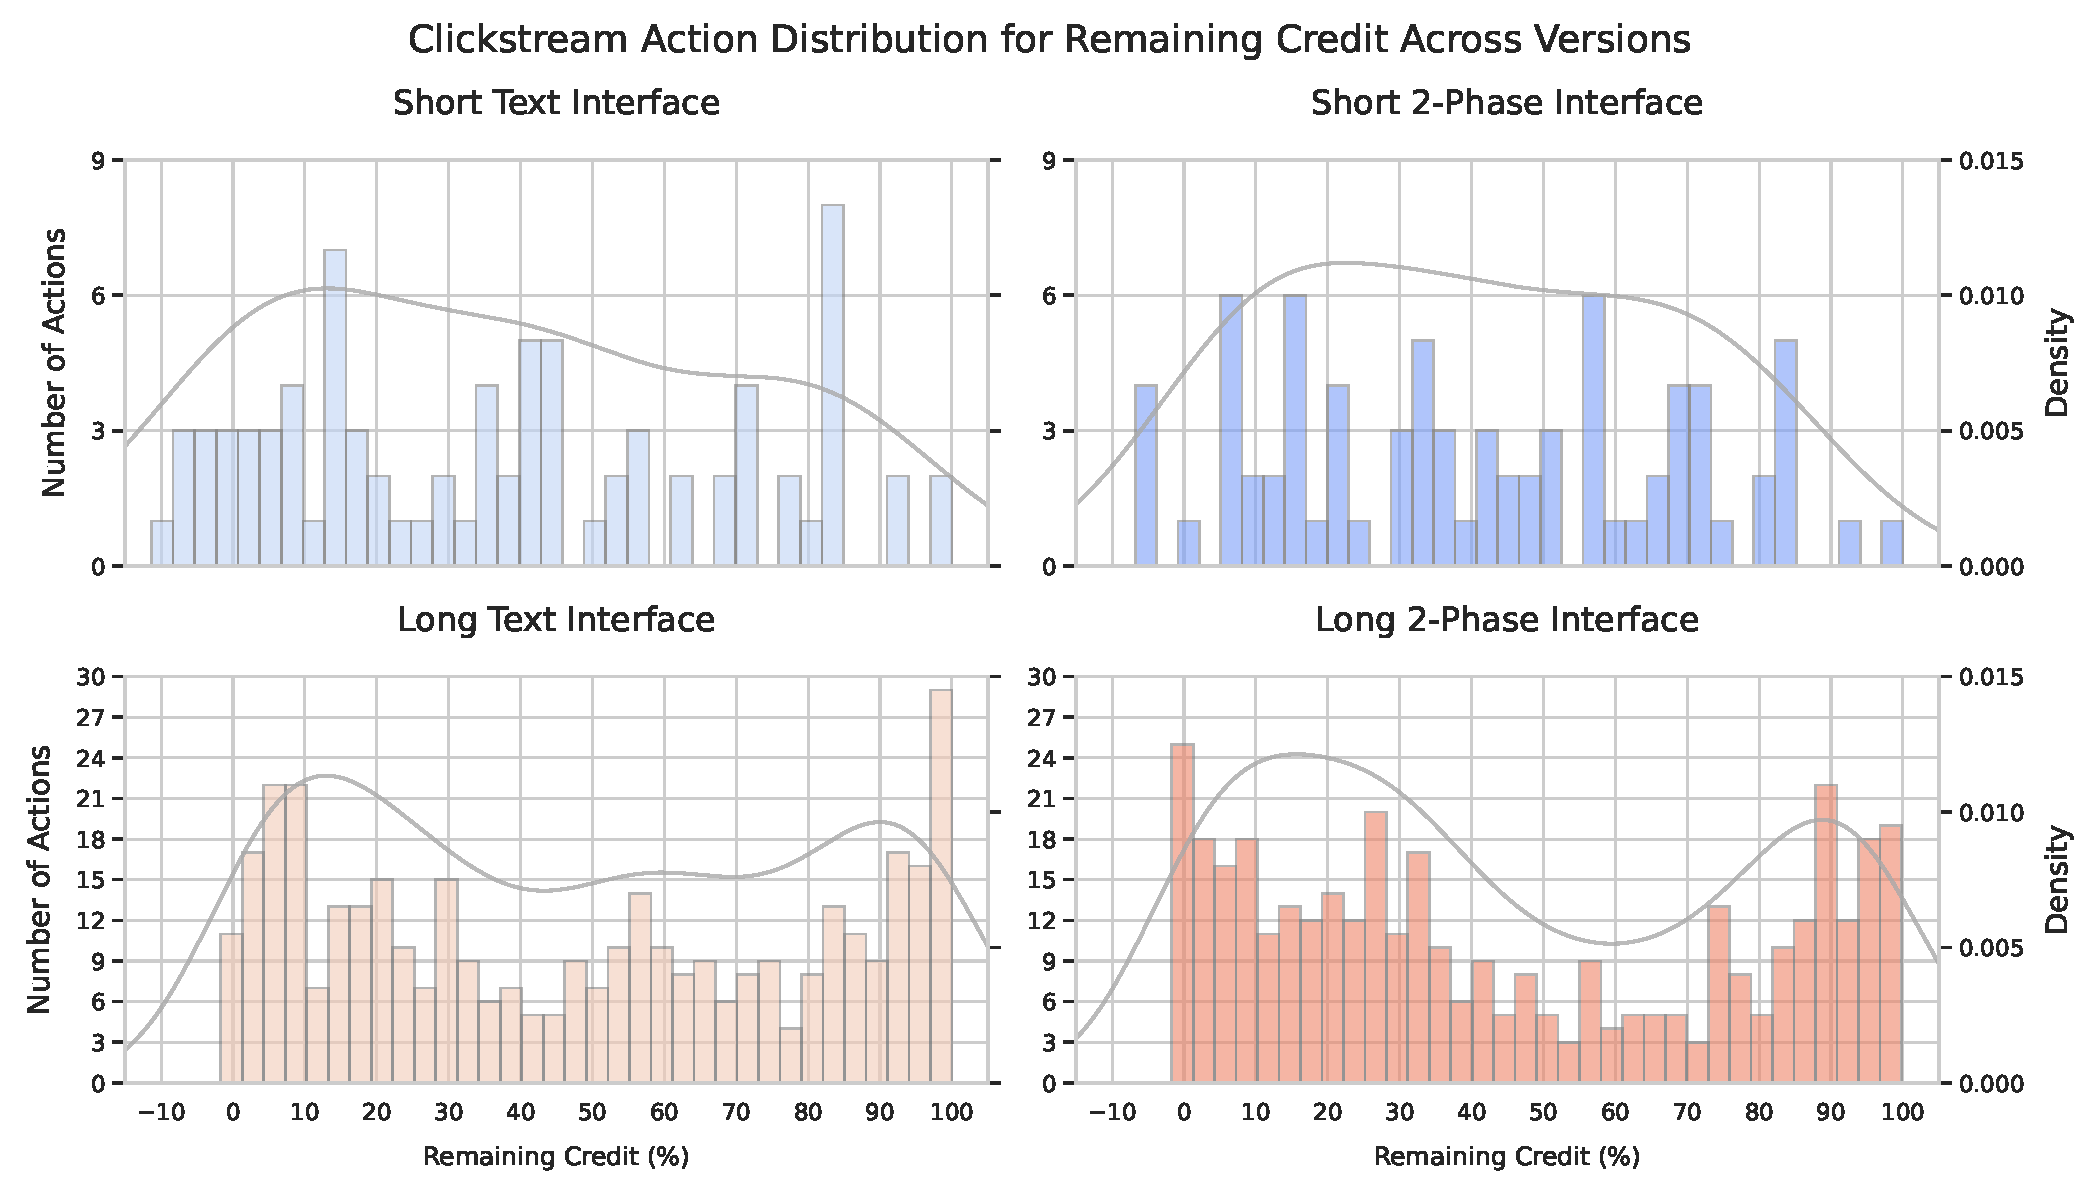
\includegraphics[width=0.9\textwidth]{content/image/results/clickstream_action_distribution.pdf}
    \caption{This plot counts the number of voting actions when there are $x$ percentages of credits remaining. A KDE plot is provided to help better understand the action distribution.}
    \Description{A four-panel histogram showing the number of voting actions across remaining credit percentages for four interface versions: Short Text, Short 2-Phase, Long Text, and Long 2-Phase. Each panel displays the number of actions on the y-axis and remaining credit on the x-axis, with an overlaid KDE curve representing density. In the top panels (Short Text and Short 2-Phase), actions are distributed relatively evenly, with small peaks around 10-20\% and 50\% remaining credit. The KDE curves show minor fluctuations. In the bottom panels (Long Text and Long 2-Phase), there are more pronounced peaks at 0-10\% and 100\% remaining credit, with broader distributions and smoother KDE curves indicating denser actions around these areas. The Long Text and Long 2-Phase interfaces exhibit more actions overall compared to the Short Text and Short 2-Phase interfaces.}
    \label{apdxfig:voting_all}
\end{figure*}

Figure~\ref{apdxfig:voting_v3_v4} presents the comparison between when participants make small or large vote adjustments at different budget levels. Revisiting the KDE curve in the second row in Figure~\ref{apdxfig:voting_all} and the curve of the second row in Figure~\ref{apdxfig:voting_v3_v4} show a stronger bimodal distribution for small vote adjustments across interfaces. In fact, the bimodal distribution is more pronounced in the two-phase interface. This suggests that participants make small adjustments both at the beginning and toward the end of the QS. However, the two-phase interface shows more frequent and faster edits towards the end. In comparison, participants also made more large vote adjustments early on that spread more equally compared to the text interface. This indicates that participants had a clearer idea of how to distribute their credits across the options.

\begin{figure*}[p]
    \centering
    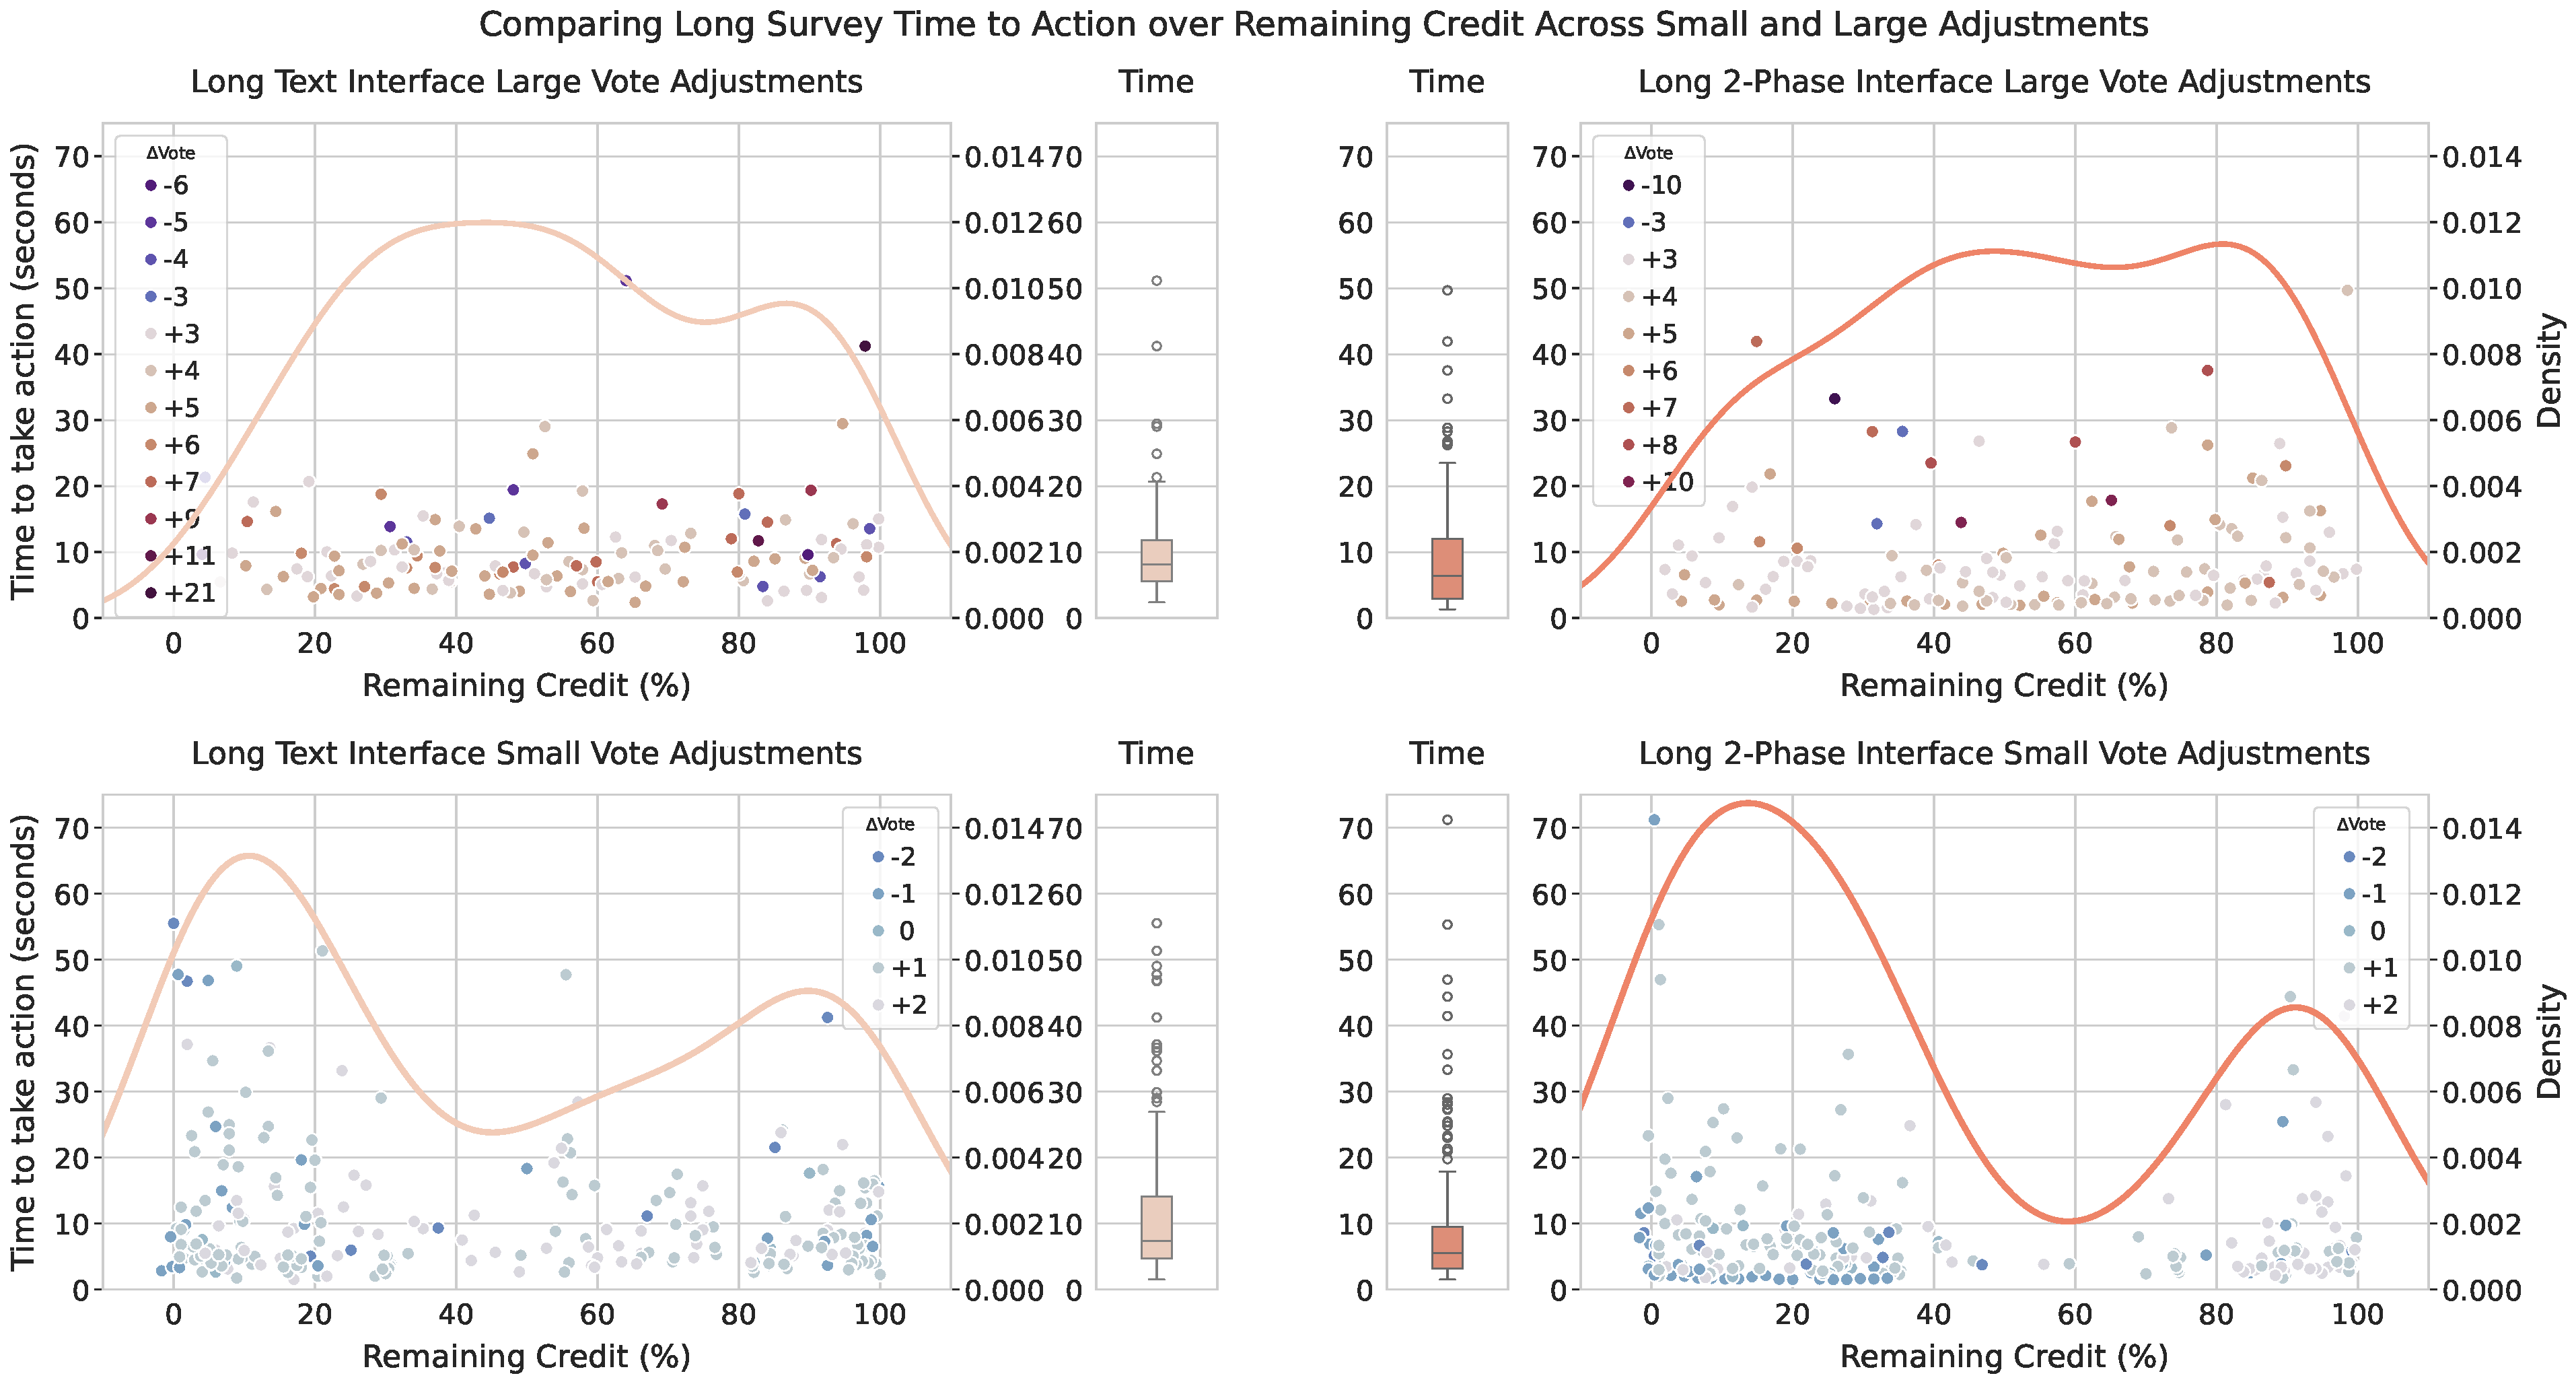
\includegraphics[width=0.9\textwidth]{content/image/results/combined_density_plots.pdf}
    \caption{This plot further separates participants' interaction behavior based on the number of votes participants adjusted. We observed a bimodal interaction pattern across long QS when small vote adjustments are made.}
    \Description{A four-panel plot comparing the time to take action in seconds over remaining credit percentages for large and small vote adjustments in the Long Text and Long 2-Phase interfaces. Each panel includes scattered points and an overlaid KDE curve. The top left panel shows large vote adjustments for the Long Text interface, with peaks in the KDE curve around 20\% and 80\% remaining credit. The top right panel shows large vote adjustments for the Long 2-Phase interface, with two peaks in the KDE curve around 10\% and 100\%. The bottom left panel shows small vote adjustments for the Long Text interface, with scattered points and peaks in the KDE curve around 10\% and 90\%. The bottom right panel shows small vote adjustments for the Long 2-Phase interface, with a KDE curve peaking around 10\% and 100\% remaining credit. Box plots on the right side of each panel summarize the distribution of time taken to adjust votes for each interface.}    
    \label{apdxfig:voting_v3_v4}
\end{figure*}

 % Done

% % Modeling Appendix
% % \section{Modeling}
\section{Modeling NASA-TLX Weighted Scores and Subscales}
\label{apdx:model_tlx}
This section first describes the hierarchical Bayesian ordinal regression model used for the NASA-TLX weighted scores and subscales. We then present the results for each subscale.

\subsection{Modeling Approach}

\subsubsection{Dependent variables}
\paragraph{NASA-TLX weighted scores} are transformed from a continuous $0$--$100$ scale to cognitive levels: low, medium, somewhat high, high, and very high, as described by~\citet{hart1988development}. This transformation helps the model adapt to sparse data. In our study, there were no participants who expressed "low" or "very high"; thus, we modeled the predictive variables as "medium," "somewhat high," and "high."

\paragraph{NASA-TLX subscale ratings} are transformed into ordinal groups using minimum frequency binning~\cite{frank2001simple}. Minimum frequency binning involves grouping adjacent response categories until each bin meets a predefined minimum number of observations. Since the subscale uses a 21-point Likert scale and we have 40 participants, the data are very sparse. Minimum frequency binning mitigates this by ensuring similar numbers of participants in each bin. We applied weighted bins across all participants within the same subscale, ensuring that each bin contained at least 10 participants.

\paragraph{Likelihood.} With these ordinal outcome variables, we designed $y_i$ as the observed ordinal category for participant $i$. Then:

\begin{equation}
    y_i \sim \text{OrderedLogistic}(\eta_i, \boldsymbol{\tau}),
    \label{eq:cog_main}
\end{equation}

where $\eta_i$ is the latent predictor, and $\boldsymbol{\tau}$ denotes the cutpoints demarcating the boundaries between the ordinal categories as in~\Cref{eq:cog_orderedTransfrom}. The cutpoints $\boldsymbol{\tau}$ ensure that $\tau_1 < \tau_2 < \cdots < \tau_{K-1}$ by construction.

\begin{equation}
    \boldsymbol{\tau} \sim \text{OrderedTransform}(\mathcal{N}(0, 1)^{K-1}),
    \label{eq:cog_orderedTransfrom}
\end{equation}

\subsubsection{Independent Variables and latent predictor}
For this model, we used three independent variables: length ($\gamma_i$, an ordinal variable), interface type ($\beta_I$, an categorical variable), and the interaction between the two ($\phi_{i,j}$) to construct the latent predictor $\eta_i$. Specifically, the latent predictor $\eta_i$ is constructed as:

\begin{equation}
    \eta_i = \alpha + \gamma_i + \beta_I[I_i] + \phi_{i,j},
    \label{eq:cog_regression}
\end{equation}

where: $\alpha$ is a global intercept drawn from $\mathcal{N}(0,1)$, $\gamma_i$ captures the (ordinal) effect of length, $\beta_I[I_i]$ is the effect for interface $I_i$, and $\phi_{i,j}$ is the interaction between length $i$ and interface $j$. 

Since length has two levels (short and long), we define the following equation to account for ordinality:
\begin{equation}
    \gamma_i = \mu_L + \beta_L \cdot L_i
    \label{eq:cog_ordinal}
\end{equation}

where $L_i \in \{0,1\}$, making $\gamma_i = \mu_L$ for the short condition and $\gamma_i = \mu_L + \beta_L$ for the long condition. We assign standard normal priors to these parameters: $\mu_L \sim \mathcal{N}(0,1)$ and $\beta_L \sim \mathcal{N}(0,1)$. 

\paragraph{Interface Effects.}
We model the interface effects using a non-centered parameterization to improve numerical stability and encourage partial pooling across the two interface levels. Specifically, we let $\mu_{\beta_I} \sim \mathcal{N}(0,1)$ and $\sigma_{\beta_I} \sim \mathrm{Exponential}(1)$ represent the shared mean and scale of the interface effects. We then sample a raw effect vector $\beta_{I_{\text{raw}}} \sim \mathcal{N}(0,1)^2.$ Combining these, we define:
\begin{equation}
    \beta_I = \mu_{\beta_I} + \sigma_{\beta_I} \cdot \beta_{I_{\text{raw}}}
    \label{eq:interface_reparam}
\end{equation}
where $\beta_I \in \mathbb{R}^2$ contains the effect for each of the two interface levels, 
and $\beta_I[I_i]$ indexes the effect for participant $i$'s interface. 

\paragraph{Interaction Effects} To capture potential interaction effects between length and interface types, we assign one interaction parameter, $\phi_{i,j}$, to each combination of length $i$ and interface $j$. Rather than sampling these $\phi_{i,j}$ directly, we employ a non-centered parameterization:
\[
  \boldsymbol{\phi} = L_{\Omega} \,\bigl(\sigma_{\phi} \odot z_{\phi}\bigr),
\]
where \(\boldsymbol{\phi}\) is a $2 \times 2$ matrix of interaction parameters (since we have 2 levels of length and 2 levels of interface), $z_{\phi} \sim \mathcal{N}(0,1)^{2\times2}$, $\sigma_{\phi} \sim \text{Exponential}(1)^{2\times2}$, and $L_{\Omega}$ is the Cholesky factor of a correlation matrix drawn from an $\text{LKJ}(2)$ prior. We then define
\[
    \phi_{i,j} 
    = 
    \bigl[\boldsymbol{\phi}\bigr]_{i,j},
\]
making $\phi_{i,j}$ a \emph{single scalar} drawn from the correlated matrix $\boldsymbol{\phi}$.

\subsubsection{Posterior predictive plots}
We conducted the Bayesian analysis using NumPyro, a widely used framework for Bayesian inference. We used Markov Chain Monte Carlo (MCMC) sampling, a method commonly applied in Bayesian inference. The model converged successfully, as evidenced by an $\hat{R}$ value of 1 for each subscale and the overall weighted TLX scores, indicating that multiple sampling chains converged. We plotted the posterior predictive distribution of the model to compare the observed data with the model's predictions. Figure~\ref{fig:observed_vs_predicted_all_subscale} shows the posterior predictions vs. observed data for the six subscales.

\begin{figure*}[h!]
    \centering
    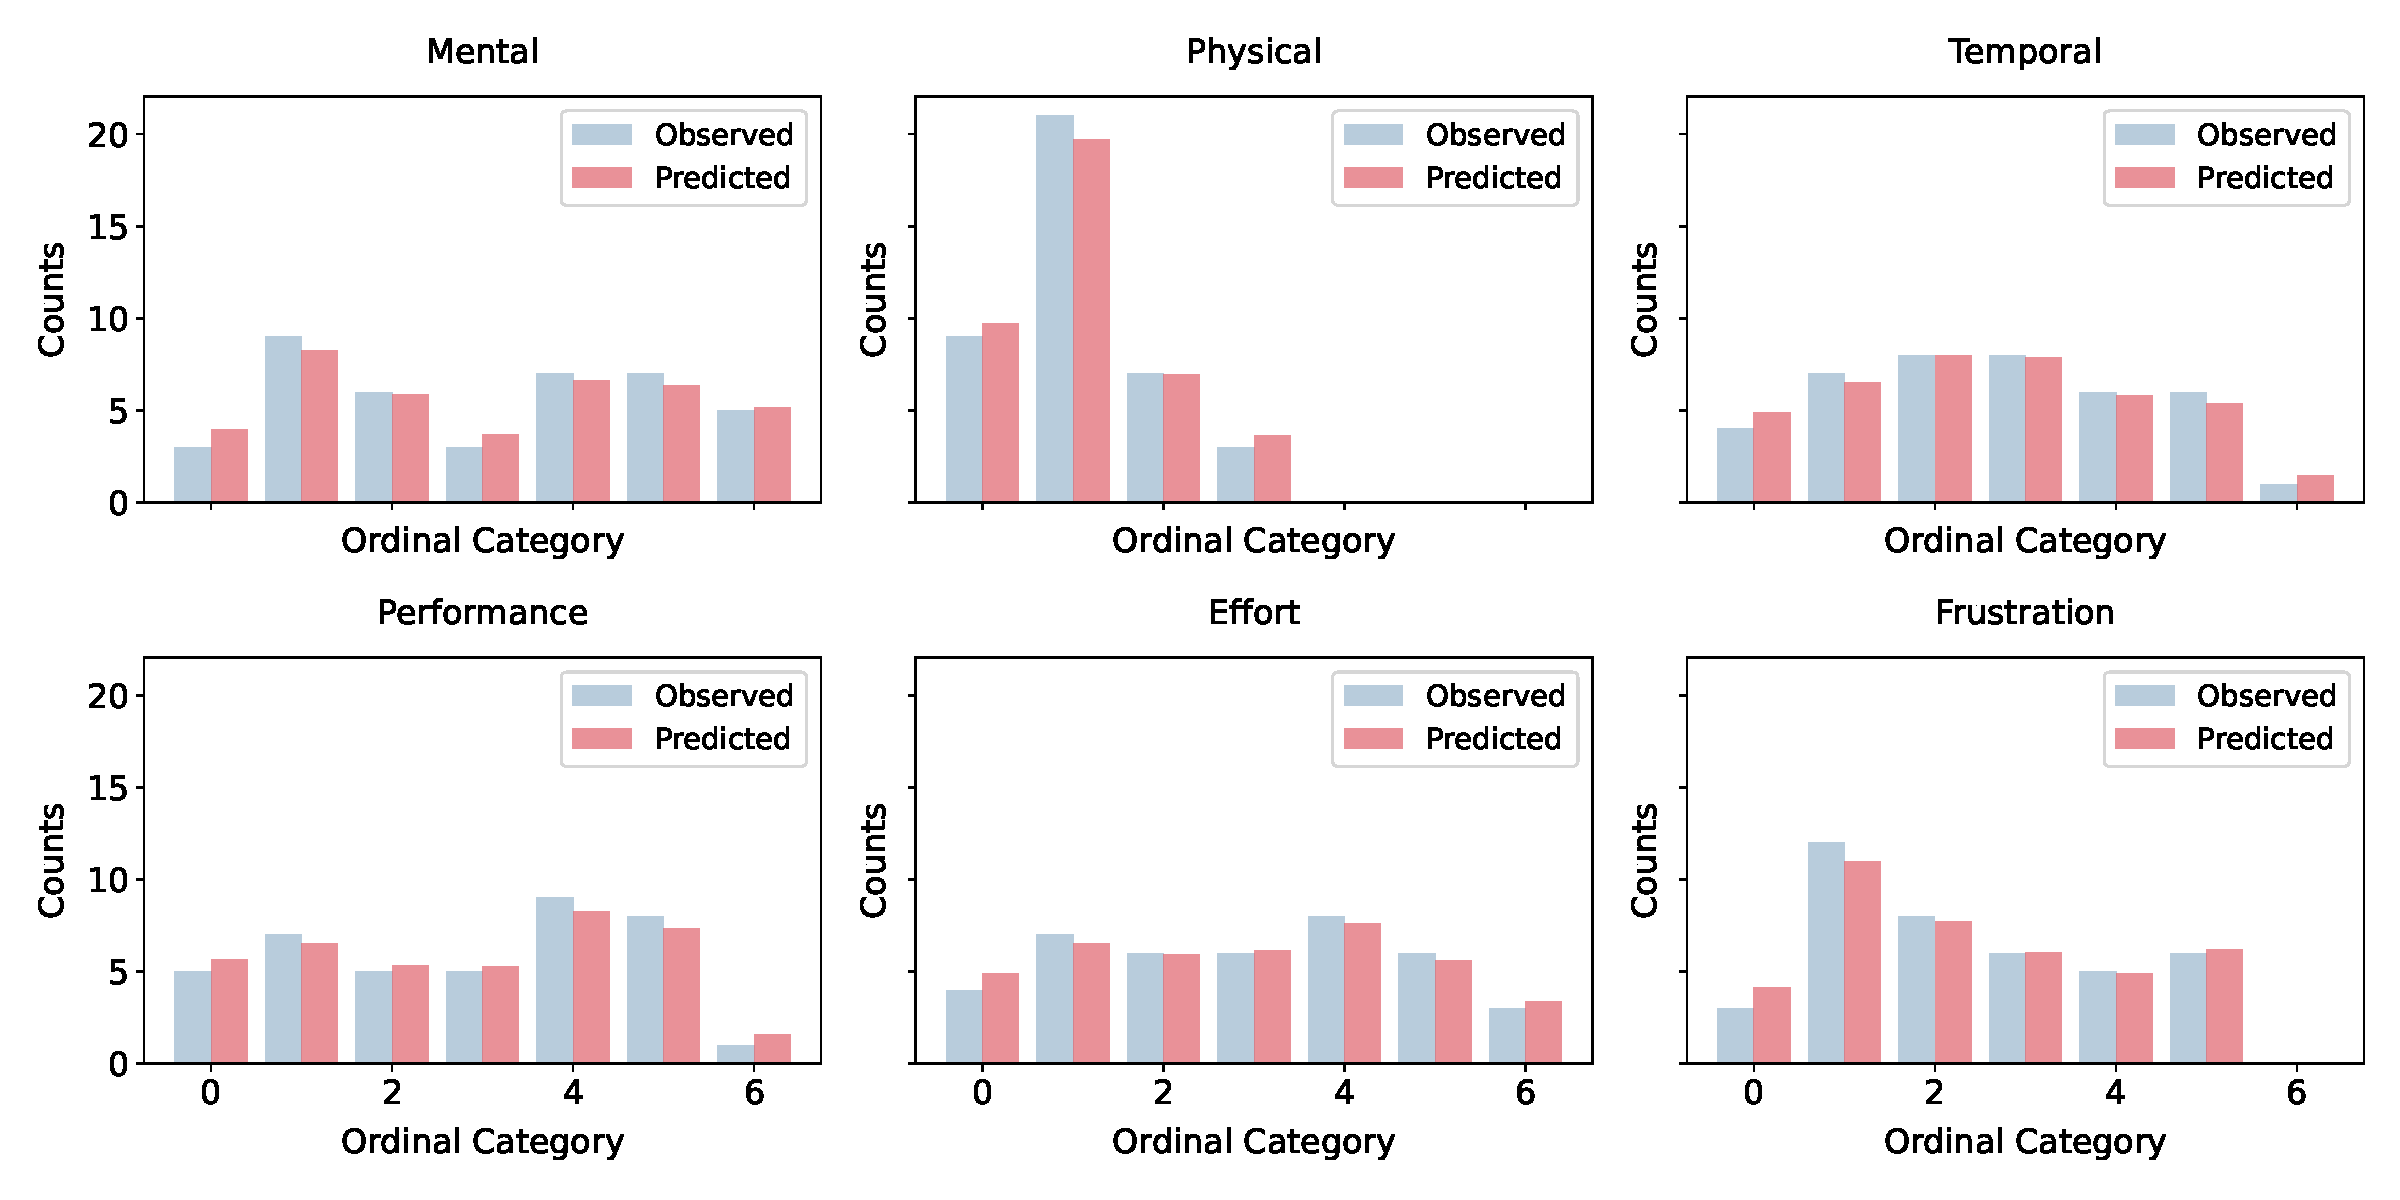
\includegraphics[width=\textwidth]{content/image/cog/observed_vs_predicted_all_subscale.pdf}
    \caption{Posterior Predictions vs. observed data for NASA-TLX subscales. The plot shows the observed number of participants in each bin compared to the posterior predictions from the model. \textbf{Takeaway of the plot}: We believe that the model is reasonable at capturing the distribution of the subscales given the sparsity of the data.}
    \Description{ A collection of bar charts comparing observed versus predicted counts across six subscales: Mental, Physical, Temporal, Performance, Effort, and Frustration. Each chart compares counts (y-axis) across ordinal categories (x-axis), highlighting discrepancies between observed and predicted values for each subscale. Bars are color-coded to distinguish observed and predicted values.}
    \label{fig:observed_vs_predicted_all_subscale}
\end{figure*}

\subsection{Model Results}
\begin{figure*}[h!]
    \centering
    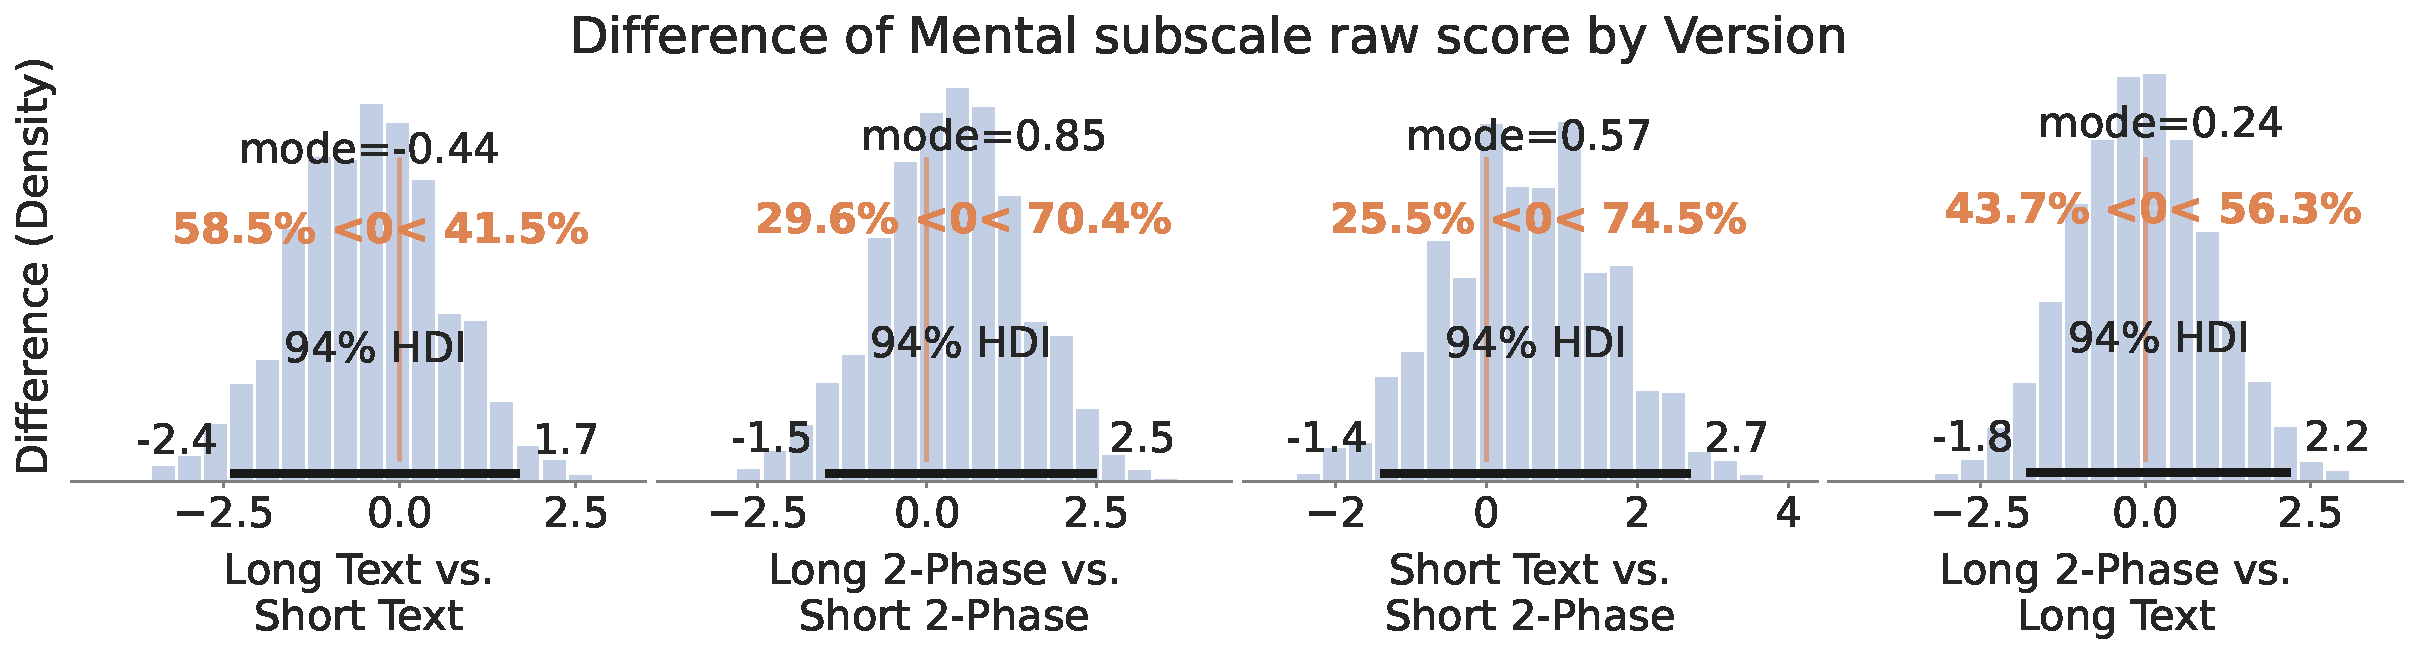
\includegraphics[width=0.75\textwidth]{content/image/cog/Mental_cog_diff_single_row.pdf}
    \caption{Differences in the mental subscale scores by version.~\textbf{Main Takeaway:} Participants in the long two-phase condition show trends to increase mental demand compared to the short two-phase. Within the short text condition, participants in the short two-phase condition show a trend to reduce mental demand.}
    \Description{A grouped panel of four histograms titled "Difference of Mental subscale raw score by Version," displaying posterior distributions of differences between various experimental conditions. Each plot shows a histogram of density (y-axis) versus difference (x-axis), with key summary statistics. Each histogram includes credible intervals, density curves, and a vertical line at zero for reference. Summary values are highlighted in orange and positioned at the top of each plot.}
    \label{fig:bayesian_mental_subscale}
\end{figure*}

\begin{figure*}[h!]
    \centering
    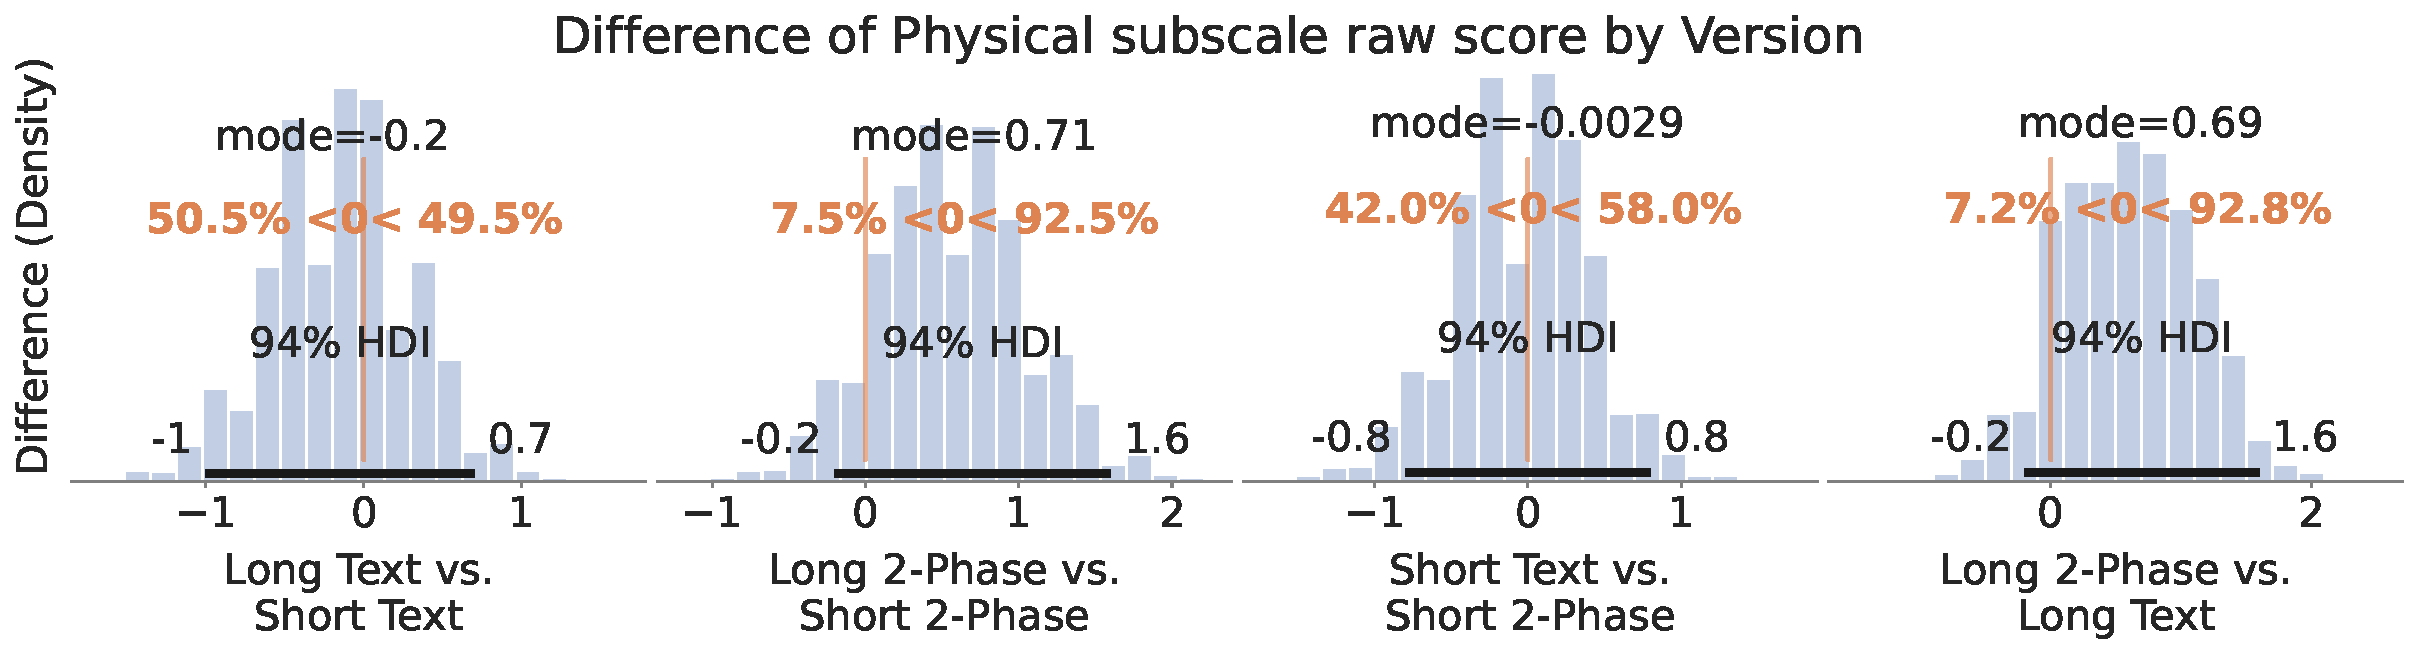
\includegraphics[width=0.75\textwidth]{content/image/cog/Physical_cog_diff_single_row.pdf}
    \caption{Differences in the physical subscale scores by version.~\textbf{Main Takeaway:} Participants in the long two-phase condition show trends to increase physical demand compared to short two-phase and long text despite the long text participants traversing higher edit distances.}
    \Description{A grouped panel of four histograms titled "Difference of Physical subscale raw score by Version," displaying posterior distributions of differences between various experimental conditions. Each plot shows a histogram of density (y-axis) versus difference (x-axis), with key summary statistics. Each histogram includes credible intervals, density curves, and a vertical line at zero for reference. Summary values are highlighted in orange and positioned at the top of each plot.}
    \label{fig:bayesian_physical_subscale}
\end{figure*}

\begin{figure*}[h!]
    \centering
    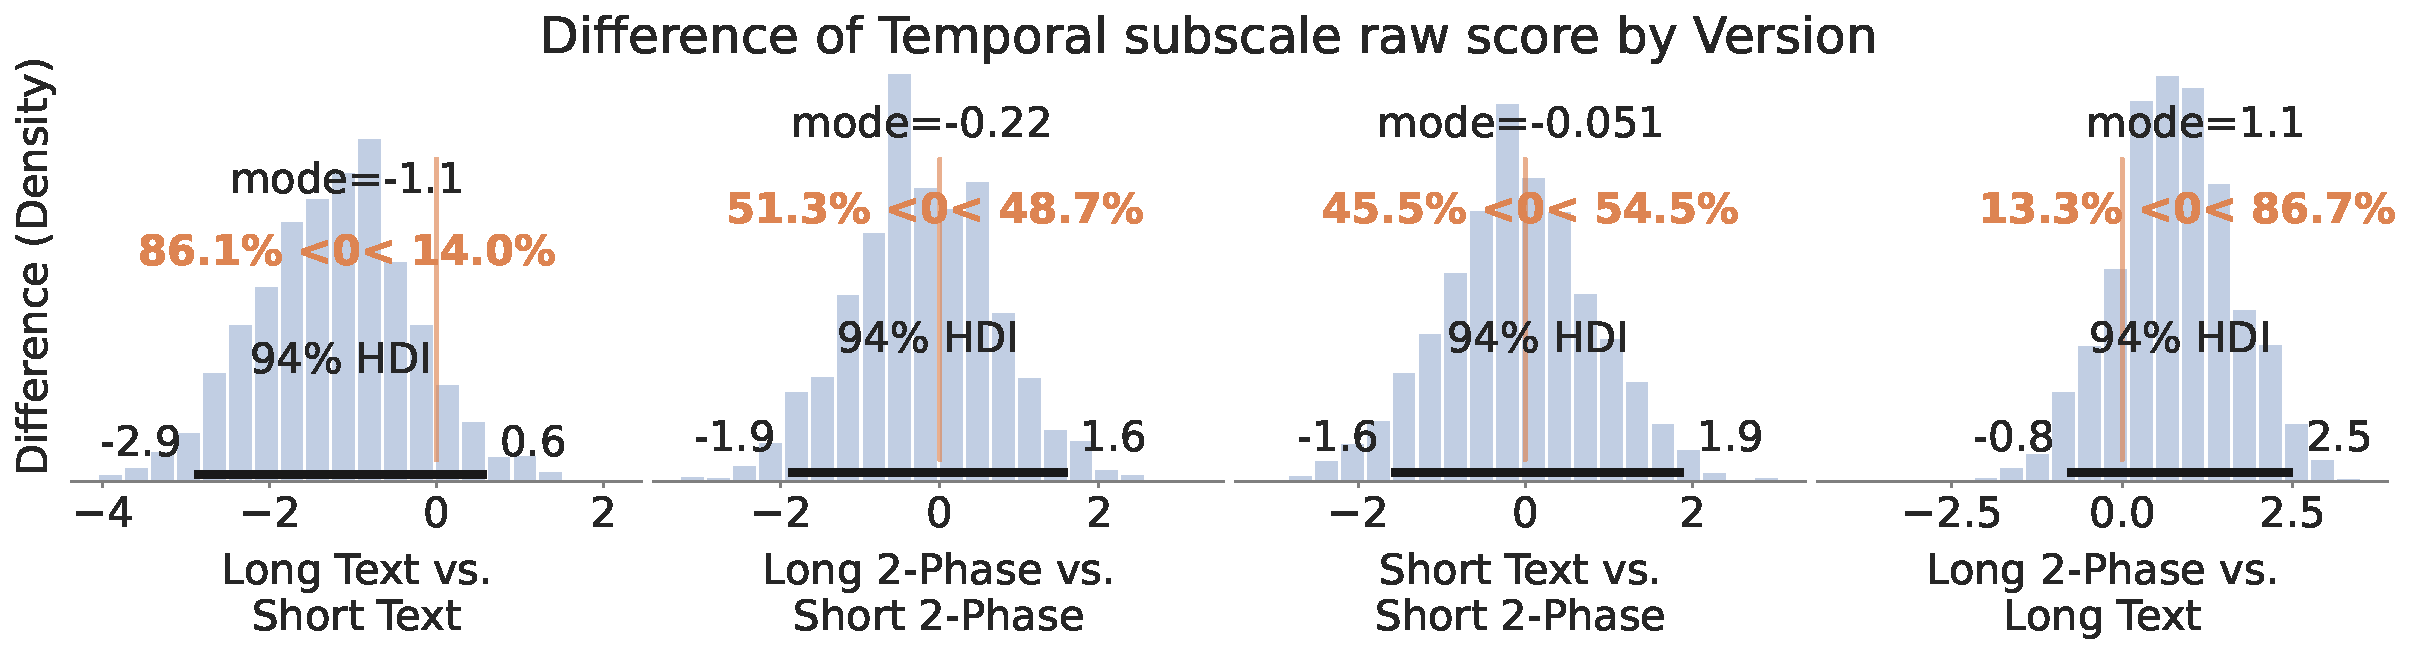
\includegraphics[width=0.75\textwidth]{content/image/cog/Temporal_cog_diff_single_row.pdf}
    \caption{Differences in the temporal subscale scores by version.~\textbf{Main Takeaway:} Participants in the long text condition show a trend that it reduces temporal demand compared to the short text condition and the long two-phase condition.}
    \Description{A grouped panel of four histograms titled "Difference of Temporal subscale raw score by Version," displaying posterior distributions of differences between various experimental conditions. Each plot shows a histogram of density (y-axis) versus difference (x-axis), with key summary statistics. Each histogram includes credible intervals, density curves, and a vertical line at zero for reference. Summary values are highlighted in orange and positioned at the top of each plot.}
    \label{fig:bayesian_temporal_subscale}
\end{figure*}

\begin{figure*}[h!]
    \centering
    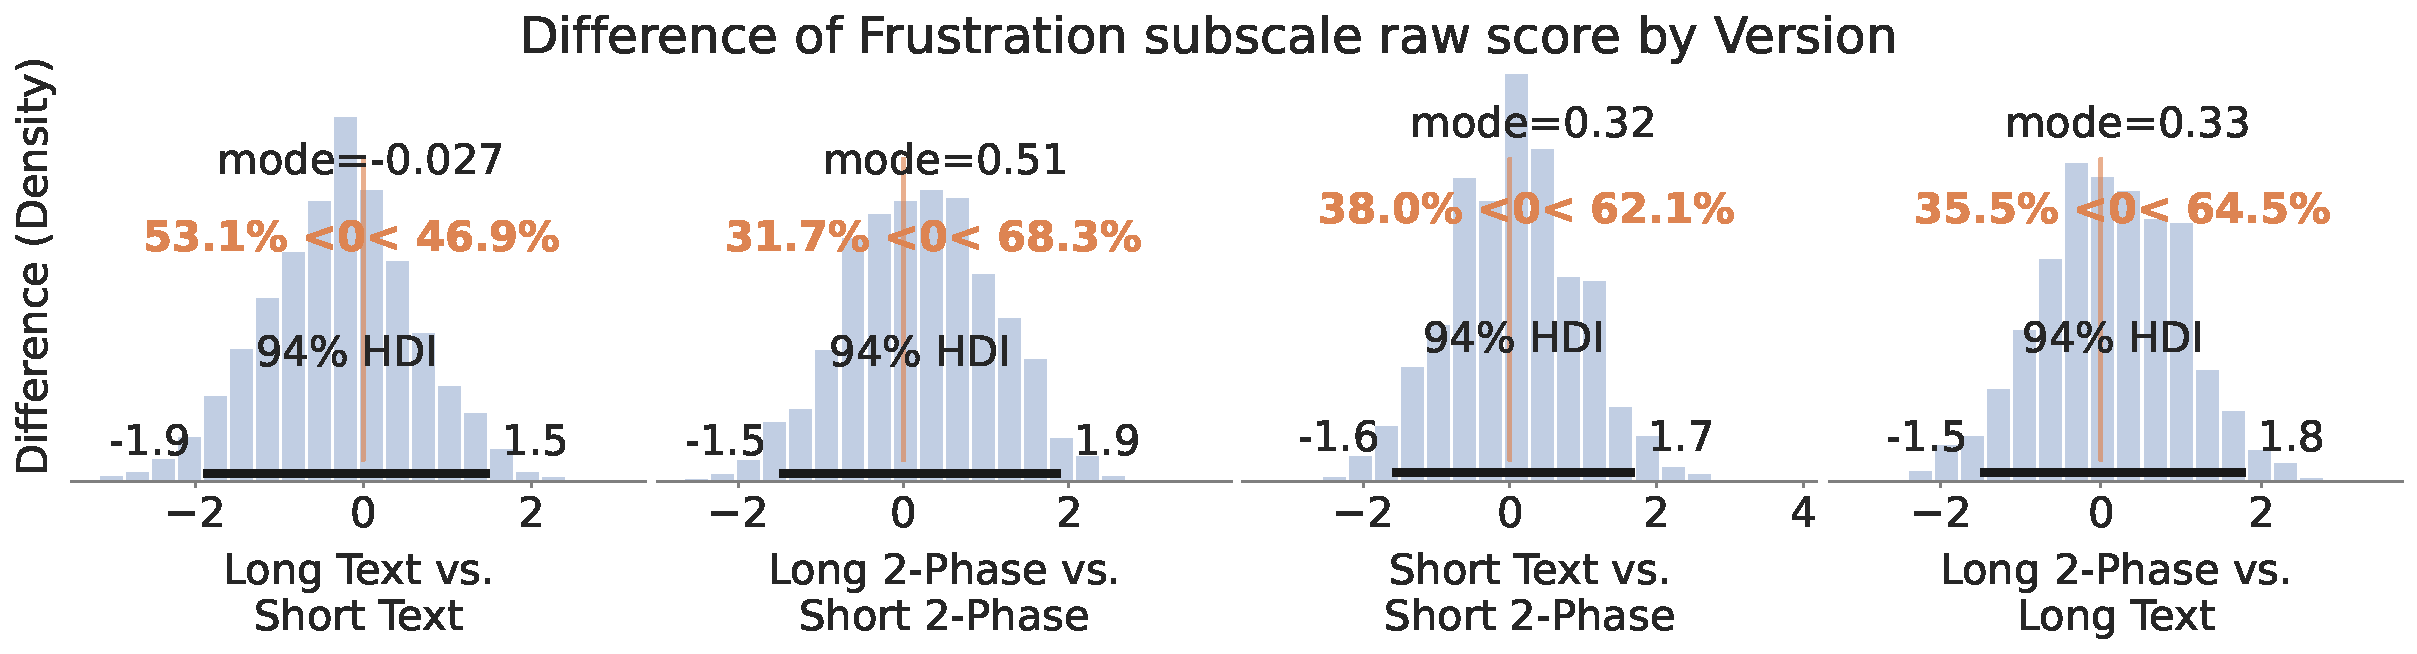
\includegraphics[width=0.75\textwidth]{content/image/cog/Frustration_cog_diff_single_row.pdf}
    \caption{Differences in the frustration subscale scores by version.~\textbf{Main Takeaway:} The model does not see a significant difference in the frustration subscale between experiment groups other than a trend for participants in the long two-phase condition to have higher frustration than the short two-phase participants.}
    \Description{A grouped panel of four histograms titled "Difference of Frustration subscale raw score by Version," displaying posterior distributions of differences between various experimental conditions. Each plot shows a histogram of density (y-axis) versus difference (x-axis), along with key summary statistics. The plots highlight the density and credible intervals for the differences, with key values marked in orange (percentages) and labeled at the top of each distribution. The vertical line at zero serves as a reference point.}
    \label{fig:bayesian_frustration_subscale}
\end{figure*}

% Section for Mental subscale
\subsubsection{Mental Subscale}
Figure~\ref{fig:bayesian_mental_subscale} shows pairwise Bayesian results from mental demand highlighted 70.4\% of posterior probability that participants in the long two-phase condition had a higher mental demand compared to the short two-phase condition. On the other hand, the short text condition had a 74.5\% posterior probability of having a higher mental demand compared to the short two-phase condition. This is additional evidence that prompted us to believe that the participants in the short two-phase participants benefited from the organization phase. The sheer number of added options in the long two-phase condition may have added additional demand to participants, leading to higher mental demand.

% Section for Physical subscale
\subsubsection{Physical Subscale}
Figure~\ref{fig:bayesian_physical_subscale} shows the pairwise comparison of the physical subscale. Notable results show that there is a 86.1\% posterior probability that the long text condition had a lesser physical demand compared to the short text condition. This is counter intuitive as the long text participants actually traversed much higher edit distances. We are not clear what prompted their self reported value and requires future research. 

% Section for Temporal subscale
\subsubsection{Temporal Subscale}
\label{sec:temporal_subscale_bayesian}
Figure~\ref{fig:bayesian_temporal_subscale} shows the pairwise comparison of the temporal subscale. The results show that the long two-phase condition once again had a 74.6\% posterior probability of having a lower temporal demand compared to the short text condition. Conversely, participants in the long two-phase condition had a 71.1\% posterior probability of having a higher temporal demand compared to the short two-phase condition, reflecting the longer time they took to complete the survey questions. We believe that the lower temporal demand in the long two-phase condition is potential indicator of the participants' satisficing behavior.

% Section for Performance subscale
\subsubsection{Performance Subscale}
We omit the pairwise comparison of the performance subscale due to the mixed signals. We focused on the qualitative results analyzed in the main text.

% Section for Effort subscale
\subsubsection{Effort Subscale}
We omit the pairwise comparison of the effort subscale due to its similarity to the mental demand subscale. 

% Section for Frustration subscale
\subsubsection{Frustration Subscale}
Figure~\ref{fig:bayesian_frustration_subscale} shows the pairwise comparison of the frustration subscale. The results show that the long two-phase condition had a 68.3\% posterior probability of having a higher frustration compared to the short two-phase condition, likely due to the added number of options to assess. 


\section{Modeling Total Time} \label{sec:apdx:model_time}

\subsubsection{Dependent Variables} The dependent variable is the total time $T_i$ spent on option $i$ measured in seconds. This measure captures both the duration participants took to vote and, where applicable, the time they spent organizing or reordering their options beforehand. We categorize the data into four experimental conditions: Short Text, Short Two-Phase, Long Text, and Long Two-Phase. These conditions are indexed by $k$, fit using separate submodels.

\subsection{Modeling Approach} We modeled the total time for each experimental condition using separate Gamma likelihood models. The Gamma distribution is well-suited for modeling positive continuous data, such as time measurements, which are often skewed and strictly positive. Equation~\ref{eq:time_main} shows the model for the total time. The shape parameter $\alpha_k$ and rate parameter $\beta_k$ were each assigned priors drawn from their own Gamma distributions, as described in Equations~\ref{eq:alpha_prior} and \ref{eq:beta_prior}.

\begin{align}
    T_i &\sim \text{Gamma}(\alpha_k, \beta_k) \label{eq:time_main} \\
    \alpha_k &\sim \text{Gamma}(2.0, 0.5) \label{eq:alpha_prior} \\
    \beta_k &\sim \text{Gamma}(1.0, 1.0) \label{eq:beta_prior}
\end{align}



% \section{Modeling Total Time} \label{sec:apdx:model_time}

% In this section, we outline how we modeled the total time ($T_i$) that participants spent considering each option in our experiment, accounting for both voting activities and, where applicable, the organization phase.

% \subsubsection{Dependent Variables} The dependent variable is the total time $T_i$, recorded for each option under consideration. This measurement includes any time participants devoted to categorizing or reordering options before making their votes.

% \subsubsection{Experimental Conditions} We distinguish four experimental conditions: Short Text, Short Two-Phase, Long Text, and Long Two-Phase. Each condition is indexed by $k$, and we fit a separate submodel for each, reflecting potential differences in the time distributions across conditions.

% \subsection{Modeling Approach} We employed a Gamma likelihood to model total time in each condition, since the Gamma distribution captures strictly positive, right-skewed data commonly observed in time measurements. Specifically, we define: \begin{align} T_i &\sim \text{Gamma}(\alpha_k, \beta_k), \label{eq:time_main} \end{align} where $\alpha_k$ is the shape parameter and $\beta_k$ is the rate parameter of the Gamma distribution for condition $k$. We assign priors to these parameters as follows: \begin{align} \alpha_k &\sim \text{Gamma}(2.0, 0.5), \label{eq:alpha_prior} \ \beta_k &\sim \text{Gamma}(1.0, 1.0). \label{eq:beta_prior} \end{align}

% By modeling each condition independently with its own shape and rate parameters, we allow the time distributions to vary flexibly across conditions, while maintaining a straightforward, interpretable structure.
\section{Modeling Edit Distance}\label{sec:apdx:model_distance}
This section presents our hierarchical Bayesian approaches for analyzing the edit distance data. We first describe a model for edit distance per option (\Cref{sec:apdx:model_distance_option}), followed by analysis for edit distance per action (\Cref{sec:apdx:model_distance_variance}). Finally, we detail a model for cumulative edit distances (\Cref{sec:apdx:model_cum_distance}).

\subsection{Model 1: Edit Distance per Option} \label{sec:apdx:model_distance_option}

\subsubsection{Likelihood}
The dependent variable in this model is the edit distance accumulated for each option, denoted by $D_i$, where $i$ refers to the $i$-th observation. Since $D_i$ must be positive, we model it using an exponential likelihood:

\begin{equation}\label{eq:distance_model_1_likelihood}
D_i \sim \text{Exponential}\bigl(\text{scale} = \lambda_i\bigr).
\end{equation}

\subsubsection{Independent variables and regression model}
We designed $\eta_i$ as the linear predictor that informs $D_i$ through the following transformation:
\begin{equation}\label{eq:transformation_model_1}
\lambda_i = \exp(\eta_i),
\end{equation}
where $\lambda_i$ is the scale (i.e., mean) parameter of the Exponential distribution, and thus must be positive.

This linear predictor:
\begin{equation}\label{eq:distance_model_1_eta}
    \eta_i = \gamma_i + \beta_I[I_i] + \phi_{ij} + U_i
\end{equation}
consists of four components: the length of the option $L_i$, interface type $I_i$, and interaction effect between both length and interface $\phi_{ij}$, and user effect $U_i$ which we describe in the following paragraphs.

\paragraph{Length.} Since length has two levels (short and long), we define:
\begin{equation}
    \gamma_i = \mu_L + \beta_L \cdot L_i 
    \label{eq:distance_model_1_eta_ordinal}
\end{equation}
where $L_i \in \{0,1\}$, making $\gamma_i = \mu_L$ for the short condition and $\gamma_i = \mu_L + \beta_L$ for the long condition. We assign standard normal priors to these parameters: $\mu_L \sim \mathcal{N}(0,1)$ and $\beta_L \sim \mathcal{N}(0,1)$. 

\paragraph{Interface.}
We model the interface effects using a non-centered parameterization to improve numerical stability and encourage partial pooling across the two interface levels. Specifically we let $\mu_{\beta_I} \sim \mathcal{N}(0,1)$ and $\sigma_{\beta_I} \sim \mathrm{HalfNormal}(0.5)$ represent the shared mean and scale of the interface effects. We then sample a raw effect vector $\beta_{I_{\text{raw}}} \sim \mathcal{N}(0,1)^2.$ Combining these, we define:
\begin{equation}
    \beta_I = \mu_{\beta_I} + \sigma_{\beta_I} \cdot \beta_{I_{\text{raw}}}
    \label{eq:distance_interface_reparam}
\end{equation}
where $\beta_I \in \mathbb{R}^2$ contains the effect for each of the two interface levels, 
and $\beta_I[I_i]$ indexes the effect for participant $i$'s interface. 

\paragraph{Interaction Effects} To capture potential interaction effects between length and interface types, we assign one interaction parameter, $\phi_{i,j}$, to each combination of length $i$ ($i \in \{0,1\}$) for short and long surveys and interface $j$ ($j \in \{0,1\}$) for the two interface types. Rather than sampling these $\phi_{i,j}$ directly, we employ a non-centered parameterization:
\[
  \boldsymbol{\phi} = L_{\Omega} \,\bigl(\sigma_{\phi} \odot z_{\phi}\bigr),
\]
where \(\boldsymbol{\phi}\) is a $2 \times 2$ matrix of interaction parameters (since we have 2 levels of length and 2 levels of interface), $z_{\phi} \sim \mathcal{N}(0,1)^{2\times2}$, $\sigma_{\phi} \sim \text{HalfNormal}(0.5)^{2\times2}$, and $L_{\Omega}$ is the Cholesky factor of a $2\times2$ correlation matrix drawn from an $\text{LKJ}(2)$ prior with shape parameter $\eta=3$. We then define
\begin{equation}
    \phi_{ij} = \bigl[\boldsymbol{\phi}\bigr]_{i,j}
\end{equation}
making $\phi_{ij}$ a \emph{single scalar} drawn from the correlated matrix $\boldsymbol{\phi}$.

\paragraph{Individual user effects.} 
Similar to the interface, we also applied a non-centered parameterization to user effects using the same approach:
\begin{equation}\label{eq:distance_model_1_user_effect}
    U_i = \mu_U + \sigma_U \cdot z_U 
\end{equation}

We assign weakly informative priors for the user effects: $\mu_U \sim \mathcal{N}(0,1)$ and $\sigma_U \sim \mathrm{Exponential}(0.5)$, which represent the shared mean and scale of the user effects. We use $z_U \sim \mathcal{N}(0,1)^{40}.$ to denote the $40$ participant's raw user effect vector. This approach allow us to capture user variations across all users.

\subsubsection{Posterior predictive plots}
Our Bayesian model converged successfully, as evidenced by an $\hat{R}$ value of 1 in the model summary. We plotted the posterior predictive distribution for the edit distance per option in Figure~\ref{fig:ppc_distance_m1}. This figure compares the models posterior predictive distribution with the observed data. 

\begin{figure}[h!]
    \centering
    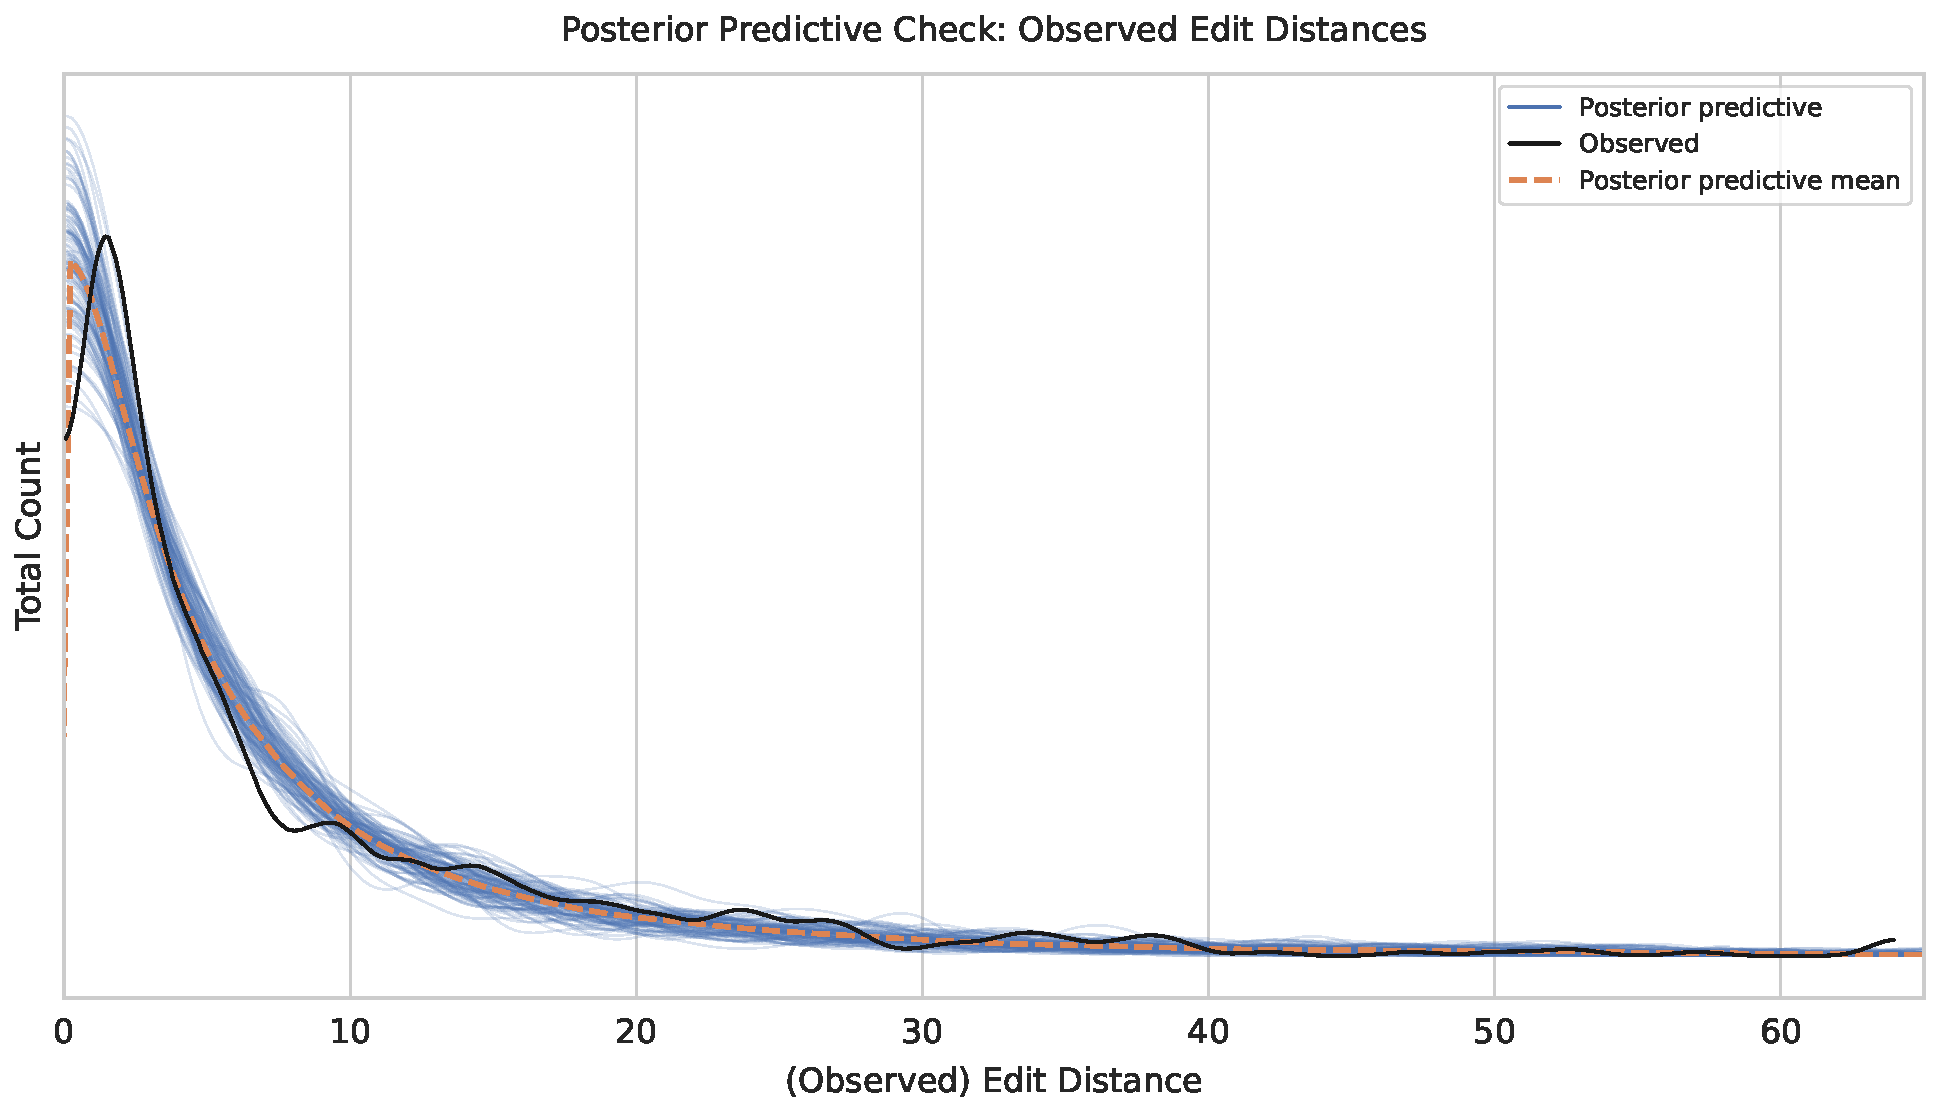
\includegraphics[width=0.45\textwidth]{content/image/distance/ppc_distance_m1.pdf}
    \caption{Posterior Predictions vs. observed data for edit distance per option. Each blue line represents a draw from the posterior distribution, while the black line represents the observed data. Dotted line represents the mean of the posterior data. \textbf{Takeaway of the plot}: We believe that the model is reasonable at capturing the distribution.}
    \Description{ A line plot titled "Posterior Predictive Check: Observed Edit Distances," comparing observed edit distances with model predictions. Multiple thin blue lines indicating individual model simulations. A solid black line representing actual observed data. A dashed orange line showing the average of posterior predictions. The plot illustrates strong alignment between observed data and the posterior predictive mean, with deviations primarily at higher edit distances. This indicates a well-calibrated model fit for most of the distribution.}
    \label{fig:ppc_distance_m1}
\end{figure}

\begin{figure*}[h!]
    \centering
    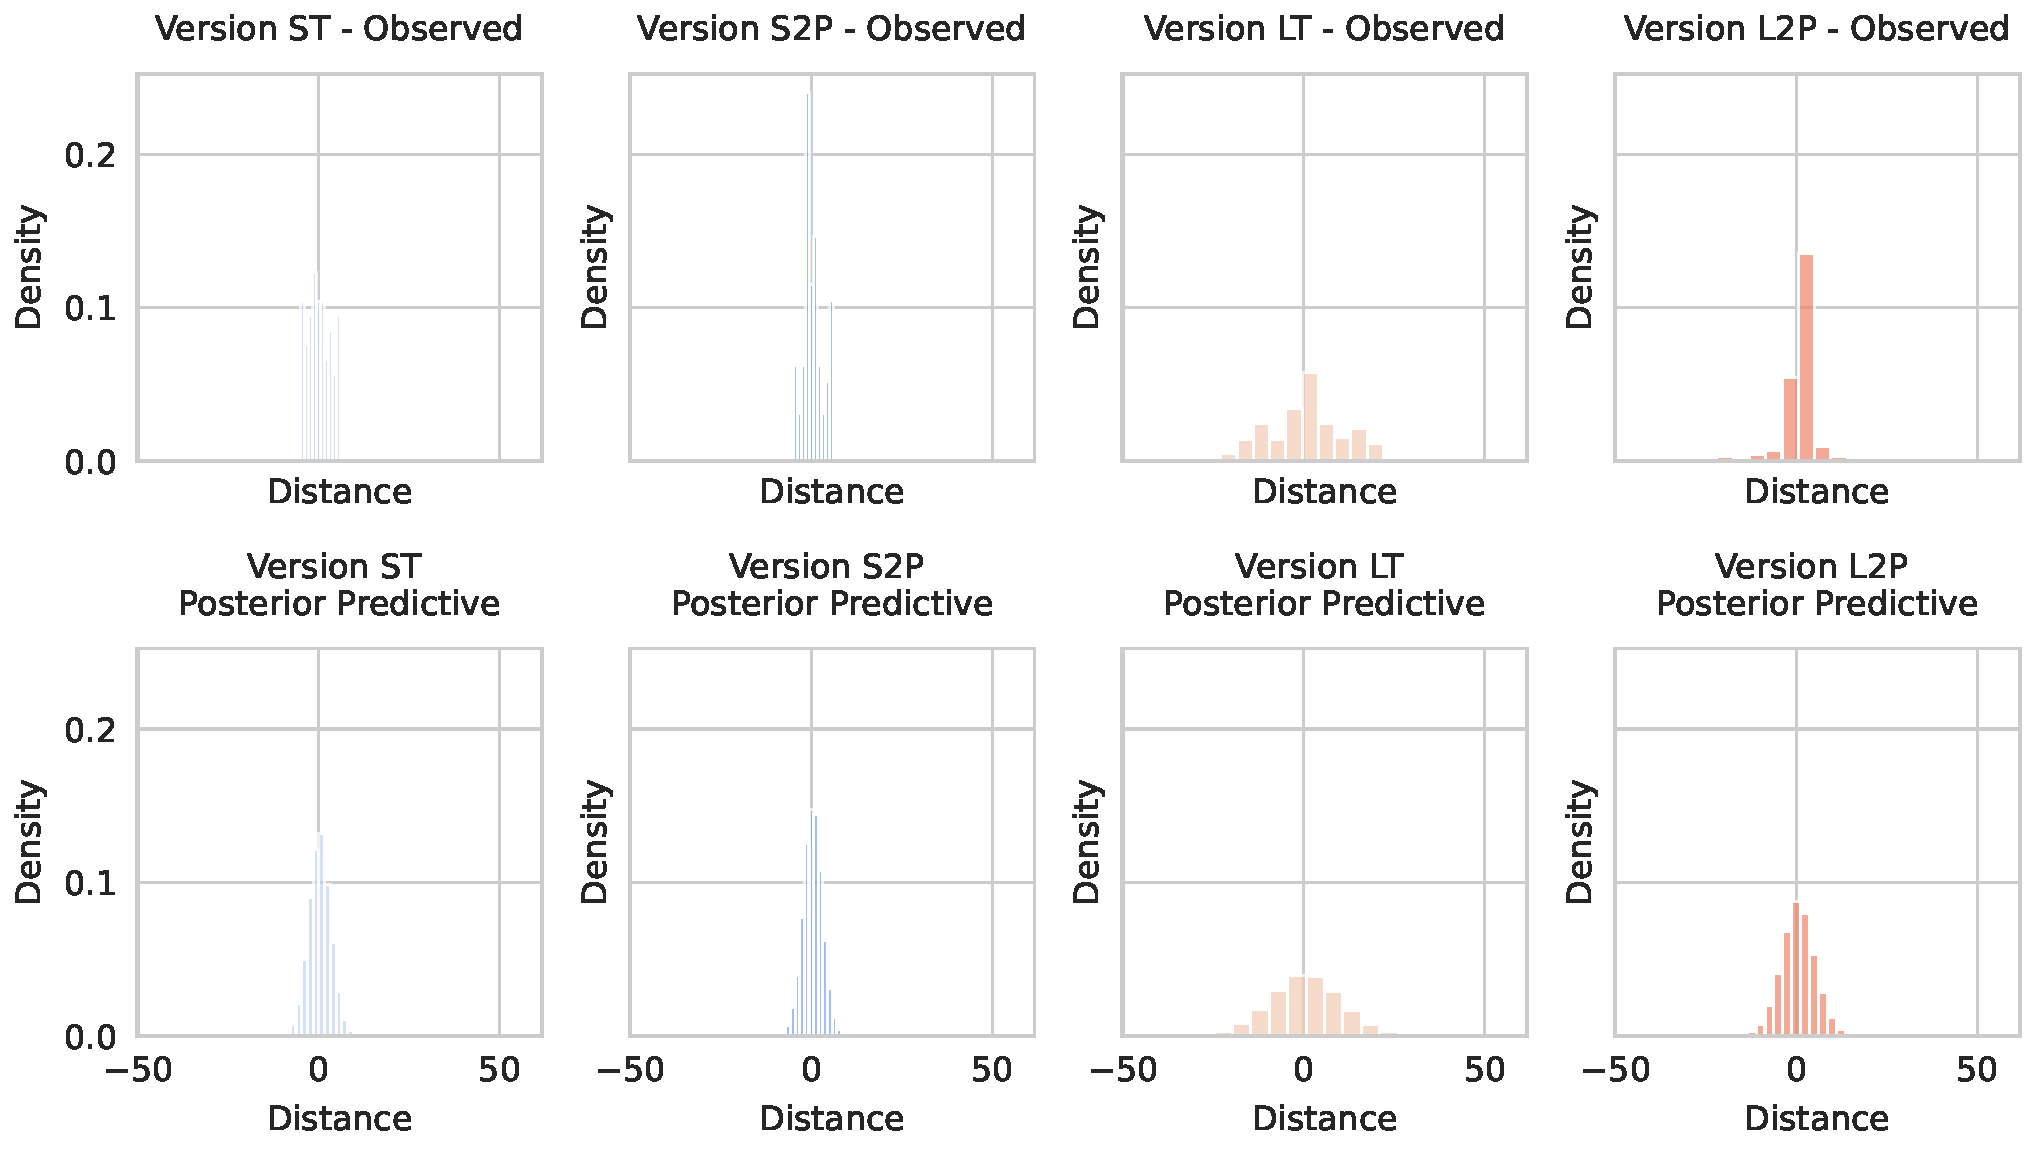
\includegraphics[width=0.75\textwidth]{content/image/distance/observed_vs_posterior_predictive_histogram_m2.pdf}
    \caption{Posterior Predictions vs. Observed Data for Edit Distance per Option. The first row represents the distribution of edit distance per version. The second row shows the posterior predictions after multiple draws \textbf{Takeaway of the plot}: We believe that the model is reasonable at capturing the shape of the distributions though being slightly conservative for extreme values at the center. Future model enhancements could re-model them with a student-t distribution.}
    \Description{
        A grid of eight density plots comparing observed and posterior predictive distributions across four model versions (ST, S2P, LT, L2P). The top row displays observed distributions, and the bottom row displays posterior predictive distributions. Each plot has "Distance" on the x-axis ranging from -50 to 50 and "Density" on the y-axis. Observed distributions are more sparse, while posterior predictive distributions are tightly centered around zero for all model versions. Differences in spread and shape are noticeable, particularly between the LT and L2P models, which show wider and more peaked distributions compared to ST and S2P.
    }

    \label{fig:observed_vs_posterior_predictive_histogram_m2}
\end{figure*}

\subsection{Model 2: Edit Distance with Separate Mean and Variance Predictors} \label{sec:apdx:model_distance_variance}

\subsubsection{Likelihood}
The dependent variable for this model is the edit distance $D_i$, where positive values indicate a downward movement and negative values indicate an upward movement. To allow for different effects on both the mean and variance, we model $D_i$ using a Normal distribution:

\begin{equation}\label{eq:distance_model_2_likelihood}
D_i \sim \mathcal{N}\bigl(\mu_i, \sigma_{\text{obs},i}\bigr)
\end{equation}

\noindent Because our aim is to capture potential differences in variability (e.g., hypothesizing that a two-phase interface might yield lower oscillation than a text-based interface), we separately model both the mean $\mu_i$ and the standard deviation $\sigma_{\text{obs},i}$.

\subsubsection{Independent variables and regression model}

We specify two linear predictors: one for the mean $\mu_i$ (Equation~\ref{eq:distance_model_2_mu}) and one for the (logged) standard deviation $\log(\sigma_{\text{obs},i})$ (Equation~\ref{eq:distance_model_2_sigma}). Both linear predictors incorporate the following factors: the length of the option $L_i$, the interface type $I_i$, an interaction term $\phi_{ij}$, and a user-specific term $U_i$.

\begin{align} 
\mu_i &= \gamma_{\mu,i} + \beta_{I,\mu}[I_i] + \phi_{\mu,ij} + U_{\mu,i}, \label{eq:distance_model_2_mu}\\
log(\sigma_{\text{obs},i}) &= \gamma_{\sigma,i} + \beta_{I,\sigma}[I_i] + \phi_{\sigma,ij} + U_{\sigma,i}. \label{eq:distance_model_2_sigma} 
\end{align}

\paragraph{Length ($L_i$).} Similar to the previous model, we continue to define length as an ordinal value. In this model, the effect for mean and variance are modeled separately. We write: 
\begin{align} 
\gamma_{\mu,i} &= \mu_{L,\mu} + \beta_{L,\mu} \cdot L_i, \label{eq:distance_model_2_gamma_mu}\\
\gamma_{\sigma,i} &= \mu_{L,\sigma} + \beta_{L,\sigma} \cdot L_i. \label{eq:distance_model_2_gamma_sigma} 
\end{align}
For both the mean and variance parts, $\mu_{L,\mu}, \beta_{L,\mu}$ and $\mu_{L,\sigma}, \beta_{L,\sigma}$ capture how option length shifts the location and scale of the distribution, respectively. We assign weakly informative normal priors:
\begin{equation}
    \mu_{L,\mu}, \beta_{L,\mu}, \mu_{L,\sigma}, \beta_{L,\sigma} \sim \mathcal{N}(0, 1).
\end{equation}


\paragraph{Interface ($I_i$).} We treat the interface type as a categorical variable with two levels. As in Model 1, we use a non-centered parameterization for numerical stability and partial pooling. For the mean part, we define: \begin{equation}\label{eq:distance_model_2_beta_I_mu} 
\beta_{I,\mu}[I_i] = \mu_{I,\mu} + \sigma_{I,\mu} \cdot z_{I,\mu}[I_i].
\end{equation} and similarly for the variance part: 
\begin{equation}\label{eq:distance_model_2_beta_I_sigma} 
\beta{I,\sigma}[I_i] = \mu_{I,\sigma} + \sigma_{I,\sigma} \cdot z_{I,\sigma}[I_i].
\end{equation} 

\noindent We place weakly informative priors on the intercepts:
\begin{align}
\mu_{I,\mu}, \beta_{I,\mu}, z_{I,\mu}, \mu_{I,\sigma}, \beta_{I,\sigma}, z_{I,\sigma} \sim \mathcal{N}(0, 1),\\
\sigma_{I,\mu}, \sigma_{I,\sigma} \sim \text{HalfNormal}(0.5).
\end{align}.

\paragraph{Interaction Effects ($\phi_{ij}$).} We hypothesize that the effect of length might vary by interface. Similar to Model 1’s approach, we employ a non-centered parameterization with an LKJ correlation prior. Specifically, for both the mean and variance parts, we define: 
\begin{align} 
\phi_{\mu,ij} &= \bigl[L_{\Omega,\mu},\bigl(\sigma_{\phi,\mu} \odot z_{\phi,\mu}\bigr)\bigr]{i,j}, \label{eq:distance_model_2_phi_mu} \\
phi{\sigma,ij} &= \bigl[L_{\Omega,\sigma},\bigl(\sigma_{\phi,\sigma} \odot z_{\phi,\sigma}\bigr)\bigr]{i,j}, \label{eq:distance_model_2_phi_sigma} 
\end{align} 
where $i \in {0,1}$ (short or long) and $j \in {0,1}$ (two interface types). We continue the use of weakly informed priors:
\begin{align}
z_{\phi,\mu}, z_{\phi,\sigma} \sim \mathcal{N}(0, 1), \sigma_{\phi,\mu}, \sigma_{\phi,\sigma} \sim \text{HalfNormal}(0.5),\\
L_{\Omega,\mu}, L_{\Omega,\sigma} \sim \text{LKJ}(3).
\end{align}

\paragraph{Individual user effects ($U_i$).} To account for participant-level variability, we follow model 1 and adopt a non-centered parameterization but allow each user to have a distinct shift on both $\mu_i$ and $\log(\sigma_{\text{obs},i})$:
\begin{align} 
U_{\mu,i} &= \mu_{U,\mu} + \sigma_{U,\mu} \cdot z_{U,\mu,i}, \label{eq:distance_model_2_user_mu}\\
U_{\sigma,i} &= \mu_{U,\sigma} + \sigma_{U,\sigma} \cdot z_{U,\sigma,i}, \label{eq:distance_model_2_user_sigma}
\end{align} 
with priors:
\begin{align}
    \mu_{U,\mu}, \beta_{U,\mu}, z_{U,\mu,i}, \mu_{U,\sigma}, \beta_{U,\sigma}, z_{U,\sigma,i} \sim \mathcal{N}(0, 1),\\
    \sigma_{U,\mu}, \sigma_{U,\sigma} \sim \text{HalfNormal}(0.5).
\end{align}

\begin{figure*}[h!]
    \centering
    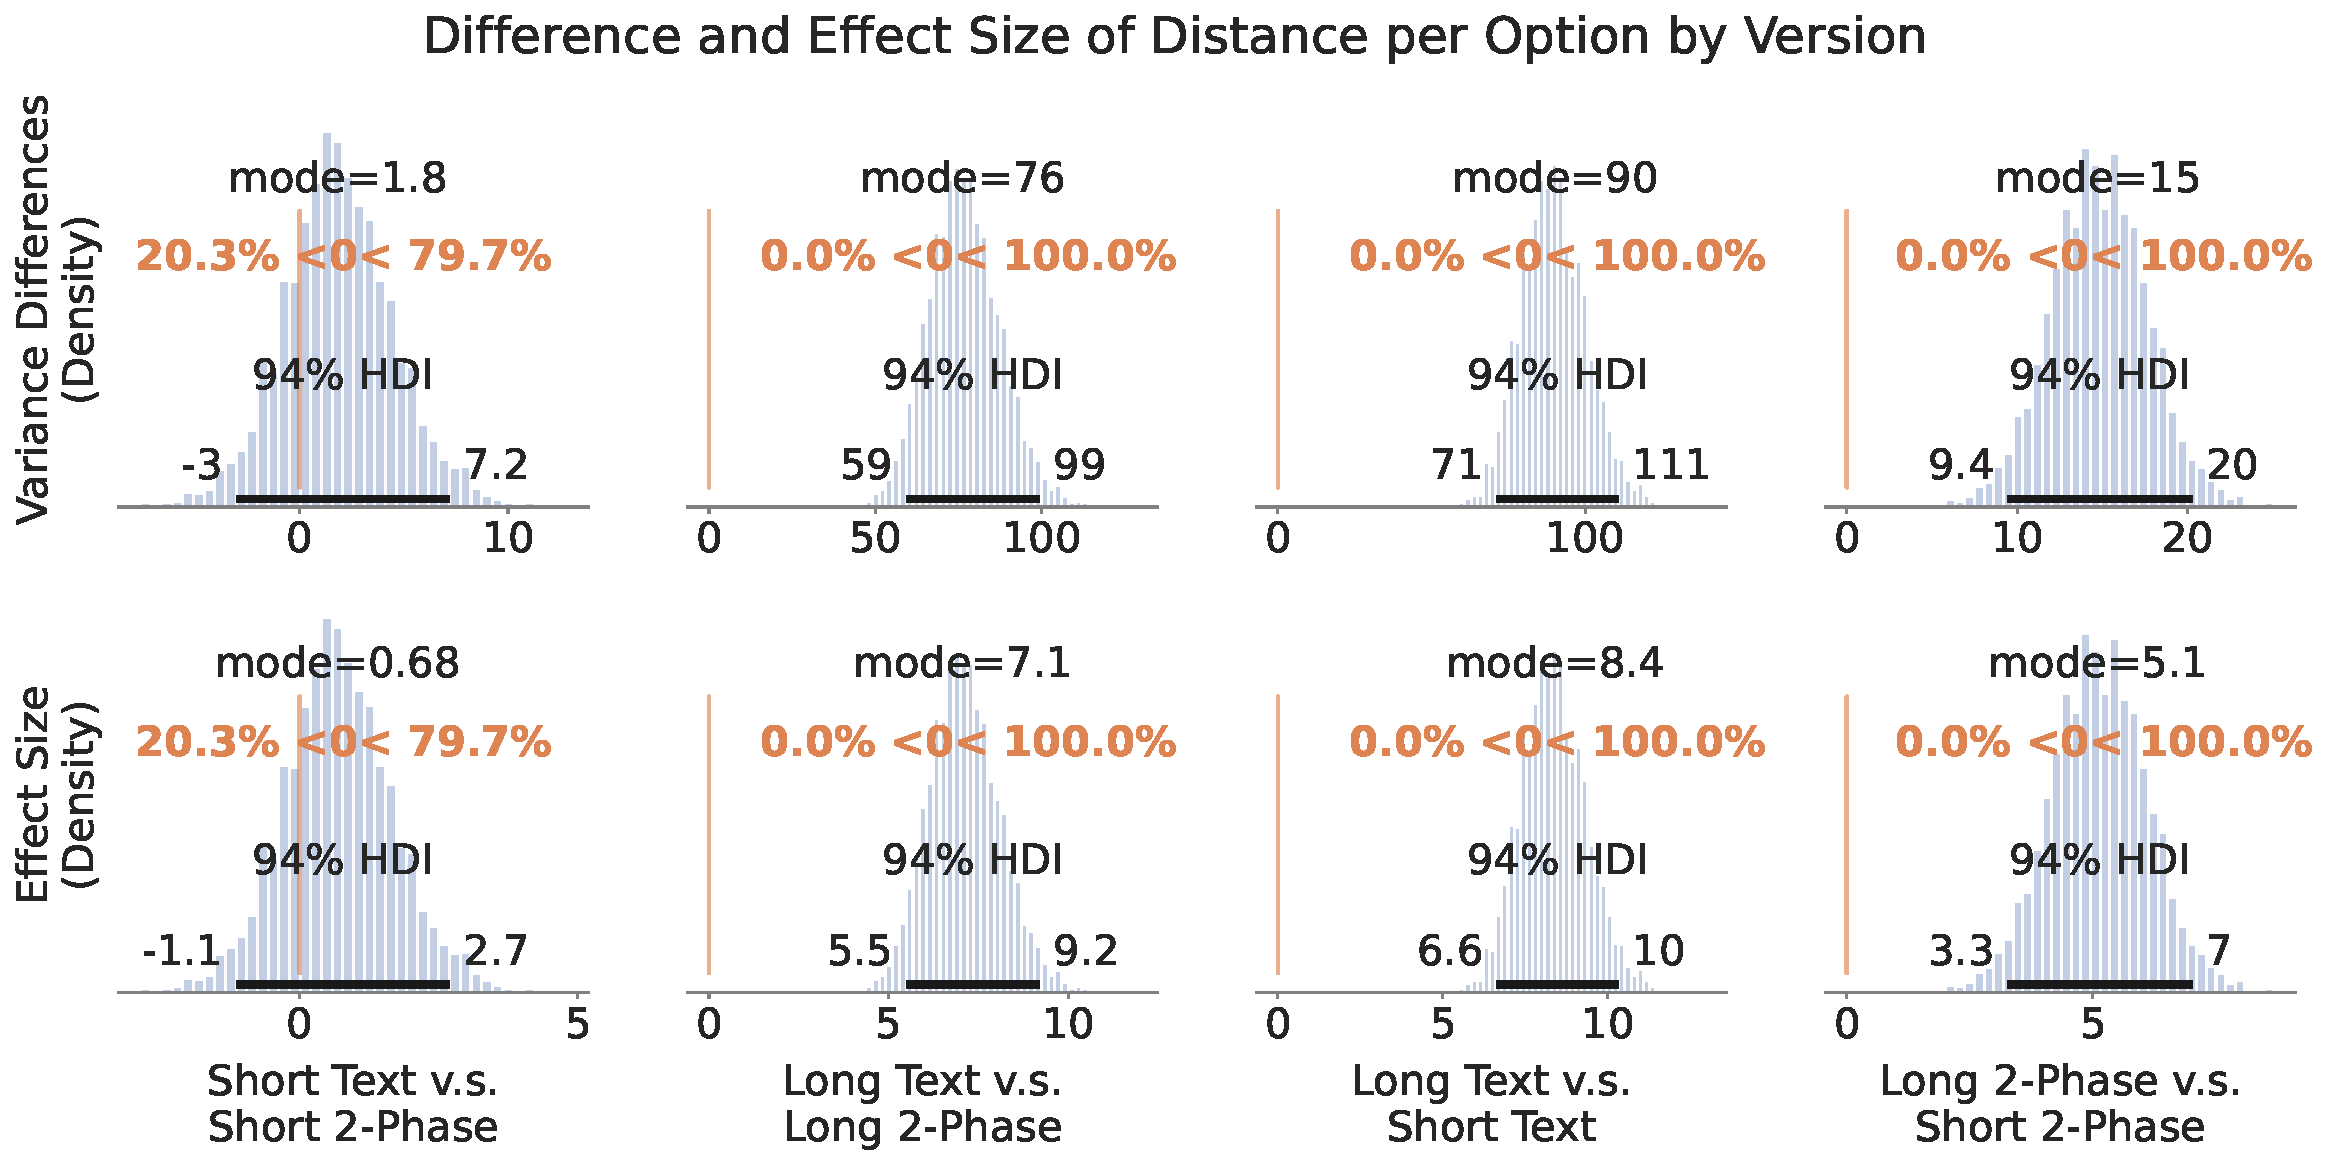
\includegraphics[width=0.8\textwidth]{content/image/distance/distance_diff_per_option_effect_size_by_version_all.pdf}
    \caption{Differences in the variance of edit distance by version.~\textbf{Main takeaway: } This plot shows that with two-phase interface, there is a reduction in edit distance variance when the number of option grows.}
    \Description{
    A grid of eight density plots showing the differences and effect sizes of distances per option by version. The top row depicts variance differences, and the bottom row depicts effect sizes, both represented as density distributions. Each column corresponds to a comparison: Short Text vs. Short 2-Phase, Long Text vs. Long 2-Phase, Long Text vs. Short Text, and Long 2-Phase vs. Short 2-Phase. Each plot includes a mode value, a 94\% Highest Density Interval (HDI), and the proportion of the distribution below and above zero. Variance difference distributions on the top row show modes ranging from 1.8 to 90, with varying HDI ranges. Effect size distributions on the bottom row have modes between 0.68 and 8.4, with all 94\% HDIs above zero except for Short Text vs. Short 2-Phase.
    }

    \label{fig:bayesian_distance_variance}
\end{figure*}

\subsubsection{Posterior predictive plots}
Our Bayesian model converged successfully, as evidenced by an $\hat{R}$ value of 1 in the model summary. We plotted the posterior predictive distribution for the edit distance per option in Figure~\ref{fig:observed_vs_posterior_predictive_histogram_m2}. This figure compares the models posterior predictive distribution with the observed data.

\subsubsection{Model Results}
Figure~\ref{fig:bayesian_distance_variance} shows the pairwise comparison of the variance of edit distance in the first row followed by the effect size in the second row. In addition to the comparison within the same survey length, we provide all pairwise comparisons. A notable result that we omit from the main text is that if we compare the variance between the long and short text, and the variance between the long and short two-phase, we see that the text group had three times the standard deviation compared to the two-phase group. This indicates that the organization phase minimize the edit distance despite the increase in survey length.

\subsection{Model 3: Long QS Cumulative Edit Distance} \label{sec:apdx:model_cum_distance}

The dependent variable for this model is the cumulative edit distance $D_i$, a positive continuous variable measured at each step within a version for each user. We modeled this to test our hypothesis that for each participant, the growth rate of the edit distance is consistent. To accommodate its positive nature, we model $D_i$ using a Truncated Normal distribution:

\begin{equation}\label{eq:model3_likelihood}
D_i \sim \text{TruncatedNormal}(\mu_i, \sigma_{\text{obs},i}, \text{lower}=0),
\end{equation}
where the observation-specific standard deviation prior is:
\begin{equation}\label{eq:model3_prior_sigma}
\sigma_{\text{obs},i} \sim \text{HalfNormal}(0.3).
\end{equation}

\subsubsection{Independent Variables and Regression Model}
We incorporate the following independent variables: the step number when completing QS ($S_i$), the interface version ($V_i$), and user-specific effects ($U_i$). The interface version and user-specific effects are modeled using hyperpriors to capture variability across groups.

The linear predictor for $D_i$ is given by:
\begin{equation}\label{eq:model3_mu}
    \mu_i = \alpha_{\text{shared}} + \beta_v[V_i] \cdot S_i + U_i \cdot S_i,
\end{equation}
where $\alpha_{\text{shared}}$ represents the global intercept, $\beta_v[V_i]$ models the interface version effects, and $U_i$ captures individual user-specific effects. The intercept is assigned the following prior:
\begin{equation}\label{eq:model3_prior_shared}
    \alpha_{\text{shared}} \sim \mathcal{N}(2.0, 0.5).
\end{equation}

\paragraph{Interface Version ($V_i$).} Interface effects are modeled as:
\begin{equation}\label{eq:model3_prior_beta}
    \beta_v[V_i] \sim \mathcal{N}(\mu_{\beta}, \sigma_{\beta}),
\end{equation}
where the hyperparameters for the interface effect distribution are:
\begin{equation}
    \mu_{\beta} \sim \mathcal{N}(0.05, 0.05), \quad \sigma_{\beta} \sim \text{HalfNormal}(0.1).
\end{equation}

\paragraph{User Effects ($U_i$).} Instead of directly sampling $U_i$, we follow the reparameterization approach:
\begin{equation}\label{eq:model3_user_mu}
    U_i = \mu_U + \sigma_U \cdot z_{U,i},
\end{equation}
where we assign weakly informative priors $\mu_U \sim \mathcal{N}(0,1)$ and $\sigma_U \sim \text{HalfNormal}(0.1)$ to represent the shared mean and scale of the user effects. The term $z_{U,i} \sim \mathcal{N}(0,1)$ captures individual user variability, allowing us to model deviations across users while maintaining a structured prior.

\subsubsection{Posterior Predictive Plots}

Our Bayesian model converged successfully, as indicated by an $\hat{R}$ value of 1 in the model summary. Figure~\ref{fig:observed_and_predicted_cumulative_distances_by_version_m3} presents the posterior predictive distribution for cumulative edit distance, demonstrating alignment between the predicted and observed data.

\begin{figure}[h!]
    \centering
    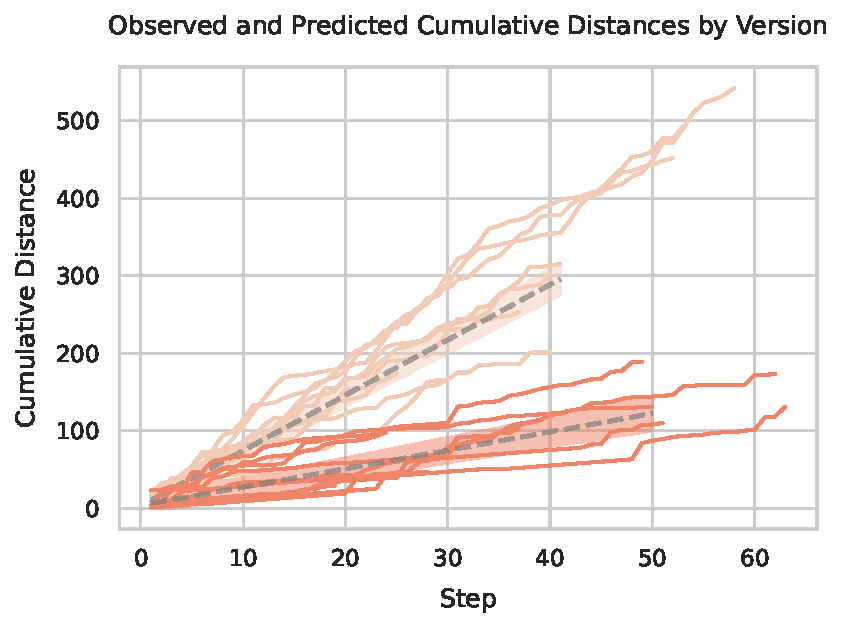
\includegraphics[width=0.45\textwidth]{content/image/distance/observed_and_predicted_cumulative_distances_by_version_m3.pdf}
    \caption{Posterior Predictions vs. observed data for cumulative edit distance. The plot showed each observed user's cumulative edit distance in different shades for the two groups of participants. Dotted line represent the posterior predictive mean. \textbf{Takeaway of the plot}: We believe that the model is reasonable at capturing slop of the cumulative trends.}
    \Description{ A line plot titled "Observed and Predicted Cumulative Distances by Version," showing cumulative distances across task steps for two conditions. Solid lines in varying shades of red and orange, representing actual cumulative distances for individual participants. Dashed lines, showing the model's predicted cumulative distances for each condition. The plot indicates alignment between observed and predicted trends, with some variability at higher cumulative distances. Predictions closely follow observed trajectories, demonstrating the model's accuracy in capturing cumulative distance patterns.}
    \label{fig:observed_and_predicted_cumulative_distances_by_version_m3}
\end{figure}





% TC:endignore

\end{document}
\endinput

